% Options for packages loaded elsewhere
% Options for packages loaded elsewhere
\PassOptionsToPackage{unicode}{hyperref}
\PassOptionsToPackage{hyphens}{url}
\PassOptionsToPackage{dvipsnames,svgnames,x11names}{xcolor}
%
\documentclass[
  letterpaper,
  DIV=11,
  numbers=noendperiod]{scrreprt}
\usepackage{xcolor}
\usepackage{amsmath,amssymb}
\setcounter{secnumdepth}{5}
\usepackage{iftex}
\ifPDFTeX
  \usepackage[T1]{fontenc}
  \usepackage[utf8]{inputenc}
  \usepackage{textcomp} % provide euro and other symbols
\else % if luatex or xetex
  \usepackage{unicode-math} % this also loads fontspec
  \defaultfontfeatures{Scale=MatchLowercase}
  \defaultfontfeatures[\rmfamily]{Ligatures=TeX,Scale=1}
\fi
\usepackage{lmodern}
\ifPDFTeX\else
  % xetex/luatex font selection
\fi
% Use upquote if available, for straight quotes in verbatim environments
\IfFileExists{upquote.sty}{\usepackage{upquote}}{}
\IfFileExists{microtype.sty}{% use microtype if available
  \usepackage[]{microtype}
  \UseMicrotypeSet[protrusion]{basicmath} % disable protrusion for tt fonts
}{}
\makeatletter
\@ifundefined{KOMAClassName}{% if non-KOMA class
  \IfFileExists{parskip.sty}{%
    \usepackage{parskip}
  }{% else
    \setlength{\parindent}{0pt}
    \setlength{\parskip}{6pt plus 2pt minus 1pt}}
}{% if KOMA class
  \KOMAoptions{parskip=half}}
\makeatother
% Make \paragraph and \subparagraph free-standing
\makeatletter
\ifx\paragraph\undefined\else
  \let\oldparagraph\paragraph
  \renewcommand{\paragraph}{
    \@ifstar
      \xxxParagraphStar
      \xxxParagraphNoStar
  }
  \newcommand{\xxxParagraphStar}[1]{\oldparagraph*{#1}\mbox{}}
  \newcommand{\xxxParagraphNoStar}[1]{\oldparagraph{#1}\mbox{}}
\fi
\ifx\subparagraph\undefined\else
  \let\oldsubparagraph\subparagraph
  \renewcommand{\subparagraph}{
    \@ifstar
      \xxxSubParagraphStar
      \xxxSubParagraphNoStar
  }
  \newcommand{\xxxSubParagraphStar}[1]{\oldsubparagraph*{#1}\mbox{}}
  \newcommand{\xxxSubParagraphNoStar}[1]{\oldsubparagraph{#1}\mbox{}}
\fi
\makeatother


\usepackage{longtable,booktabs,array}
\usepackage{calc} % for calculating minipage widths
% Correct order of tables after \paragraph or \subparagraph
\usepackage{etoolbox}
\makeatletter
\patchcmd\longtable{\par}{\if@noskipsec\mbox{}\fi\par}{}{}
\makeatother
% Allow footnotes in longtable head/foot
\IfFileExists{footnotehyper.sty}{\usepackage{footnotehyper}}{\usepackage{footnote}}
\makesavenoteenv{longtable}
\usepackage{graphicx}
\makeatletter
\newsavebox\pandoc@box
\newcommand*\pandocbounded[1]{% scales image to fit in text height/width
  \sbox\pandoc@box{#1}%
  \Gscale@div\@tempa{\textheight}{\dimexpr\ht\pandoc@box+\dp\pandoc@box\relax}%
  \Gscale@div\@tempb{\linewidth}{\wd\pandoc@box}%
  \ifdim\@tempb\p@<\@tempa\p@\let\@tempa\@tempb\fi% select the smaller of both
  \ifdim\@tempa\p@<\p@\scalebox{\@tempa}{\usebox\pandoc@box}%
  \else\usebox{\pandoc@box}%
  \fi%
}
% Set default figure placement to htbp
\def\fps@figure{htbp}
\makeatother





\setlength{\emergencystretch}{3em} % prevent overfull lines

\providecommand{\tightlist}{%
  \setlength{\itemsep}{0pt}\setlength{\parskip}{0pt}}



 


\KOMAoption{captions}{tableheading}
\makeatletter
\@ifpackageloaded{bookmark}{}{\usepackage{bookmark}}
\makeatother
\makeatletter
\@ifpackageloaded{caption}{}{\usepackage{caption}}
\AtBeginDocument{%
\ifdefined\contentsname
  \renewcommand*\contentsname{Table of contents}
\else
  \newcommand\contentsname{Table of contents}
\fi
\ifdefined\listfigurename
  \renewcommand*\listfigurename{List of Figures}
\else
  \newcommand\listfigurename{List of Figures}
\fi
\ifdefined\listtablename
  \renewcommand*\listtablename{List of Tables}
\else
  \newcommand\listtablename{List of Tables}
\fi
\ifdefined\figurename
  \renewcommand*\figurename{Figure}
\else
  \newcommand\figurename{Figure}
\fi
\ifdefined\tablename
  \renewcommand*\tablename{Table}
\else
  \newcommand\tablename{Table}
\fi
}
\@ifpackageloaded{float}{}{\usepackage{float}}
\floatstyle{ruled}
\@ifundefined{c@chapter}{\newfloat{codelisting}{h}{lop}}{\newfloat{codelisting}{h}{lop}[chapter]}
\floatname{codelisting}{Listing}
\newcommand*\listoflistings{\listof{codelisting}{List of Listings}}
\makeatother
\makeatletter
\makeatother
\makeatletter
\@ifpackageloaded{caption}{}{\usepackage{caption}}
\@ifpackageloaded{subcaption}{}{\usepackage{subcaption}}
\makeatother
\usepackage{bookmark}
\IfFileExists{xurl.sty}{\usepackage{xurl}}{} % add URL line breaks if available
\urlstyle{same}
\hypersetup{
  pdftitle={Rhio Bimo Prakoso S},
  pdfauthor={13523123 Rhio Bimo Prakoso S},
  colorlinks=true,
  linkcolor={blue},
  filecolor={Maroon},
  citecolor={Blue},
  urlcolor={Blue},
  pdfcreator={LaTeX via pandoc}}


\title{Rhio Bimo Prakoso S}
\usepackage{etoolbox}
\makeatletter
\providecommand{\subtitle}[1]{% add subtitle to \maketitle
  \apptocmd{\@title}{\par {\large #1 \par}}{}{}
}
\makeatother
\subtitle{Portfolio Asesmen II-2100}
\author{13523123 Rhio Bimo Prakoso S}
\date{2026-09-12}
\begin{document}
\maketitle

\renewcommand*\contentsname{Table of contents}
{
\hypersetup{linkcolor=}
\setcounter{tocdepth}{2}
\tableofcontents
}

\bookmarksetup{startatroot}

\chapter*{HEWWWOOO\textasciitilde\textasciitilde! :3}\label{hewwwooo-3}
\addcontentsline{toc}{chapter}{HEWWWOOO\textasciitilde\textasciitilde!
:3}

\markboth{HEWWWOOO\textasciitilde\textasciitilde!
:3}{HEWWWOOO\textasciitilde\textasciitilde! :3}

\begin{figure}[H]

{\centering \includegraphics[width=1\linewidth,height=\textheight,keepaspectratio]{./images/RBPS-1.jpg}

}

\caption{Rhio Bimo P S}

\end{figure}%

\textbf{``\emph{Whatever show holds a special place in your heart are
special because that's the person you are, so don't forget that.}''}

\begin{itemize}
\tightlist
\item
  Gigguk
\end{itemize}

\bookmarksetup{startatroot}

\chapter{UTS-1 All About Me}\label{uts-1-all-about-me}

\begin{figure}[H]

{\centering \includegraphics[width=1\linewidth,height=\textheight,keepaspectratio]{All_About_me/../images/RBPS.jpeg}

}

\caption{Rhio Bimo P S - Hero}

\end{figure}%

Aku \textbf{Rhio Bimo Prakoso S}, mahasiswa \textbf{Informatika} di
\textbf{Institut Teknologi Bandung}. Aku menulis halaman ini sebagai
pengenalan singkat---versi profesional tapi santai, dengan suara orang
pertama (aku). Bidang utamaku seputar komputasi dan pemrograman; di sisi
lain aku juga menyukai dunia kreatif khas Jepang: voice acting,
dressing, choreography, drawing, hingga 3D modelling/design.

\begin{quote}
\emph{Whatever show holds a special place in your heart are special
because that's the person you are, so don't forget that.} - Gigguk
\end{quote}

\section{Sorotan Singkat}\label{sorotan-singkat}

\begin{itemize}
\tightlist
\item
  Mulai kuliah di \textbf{ITB} tahun \textbf{2023}.
\item
  Berpartisipasi dalam \textbf{3D animation} untuk video \textbf{``Ash
  Again -- Gawr Gura.''}
\item
  \textbf{Silver Medal} pada \textbf{International Scientific Technology
  and Engineering Competition}.
\end{itemize}

\section{Minat Utama}\label{minat-utama}

\begin{itemize}
\tightlist
\item
  Anime \& budaya pop Jepang
\item
  3D Modelling / 3D Design
\item
  Cybersecurity
\end{itemize}

Blog/Website: \url{https://roxytea.wixsite.com/tarbyultima}\\
Instagram: \textbf{(\textbf{rhio\_bimo?})} ・ X:
\textbf{(\textbf{Rhio\_Bimo?})} ・ YouTube:
\url{https://www.youtube.com/@rhio_bimo}\\
Email: \textbf{13523123@std.stei.itb.ac.id}

\section{Perjalanan \& Pelajaran}\label{perjalanan-pelajaran}

Aku melewati beberapa fase yang membentuk cara pandangku:

\begin{itemize}
\tightlist
\item
  \textbf{2012 --- Ketemu Anime Jepang.} Dari sini aku belajar bahwa
  perspektif manusia itu luas; cerita bisa membuka empati dan cara
  pikir.
\item
  \textbf{2016--2017 --- Pengalaman dibully saat SD.} Aku jadi mengamati
  sifat manusia dan dinamika sosial dengan lebih jernih.
\item
  \textbf{Masa SMA --- Depresi \& pemulihan mandiri.} Aku mendalami
  psikologi dan memahami diriku lebih baik. (Tidak menggantikan bantuan
  profesional; ini sekadar catatan perjalanan pribadiku.)
\item
  \textbf{Masa SMA --- Menghadapi nepotisme.} Dari sini aku belajar
  tentang realita politik---baik di negara maupun mikro-komunitas.
\end{itemize}

Semua titik di atas membentuk \emph{narrative identity} versiku:
cenderung \textbf{agensi} (belajar mengambil kendali) dan
\textbf{penebusan} (mengolah pengalaman sulit jadi pelajaran yang
berguna).

\section{Prinsip yang Aku Pegang}\label{prinsip-yang-aku-pegang}

\begin{itemize}
\tightlist
\item
  \textbf{Jangan cepat relax} sebelum ada hasil yang konkret dan stabil.
\item
  \textbf{Buat atasan nyaman} (jangan berlebihan pamer kemampuan).
\item
  \textbf{Semakin banyak bicara, semakin besar peluang salah bicara.}
\item
  \textbf{Keep people off-balance}---jaga tujuan strategis, dan kalau
  perlu diungkap, \textbf{buatlah berkesan.}
\item
  \textbf{Jangan sok paling pintar.} Lebih enak merendah, fokus ke
  hasil.
\end{itemize}

\section{Hobi \& Hal yang Kusukai}\label{hobi-hal-yang-kusukai}

\begin{itemize}
\tightlist
\item
  Nonton YouTube
\item
  Baca Manga/Manhwa
\item
  Edit video \& brainstorming ide
\end{itemize}

\section{Figur \& Karakter yang
Menginspirasi}\label{figur-karakter-yang-menginspirasi}

\begin{itemize}
\tightlist
\item
  \textbf{Focalor} (Genshin), \textbf{Cifera} (Honkai: Star Rail),
  \textbf{Amelia Watson} \& \textbf{Gawr Gura} (VTuber),
  \textbf{Carthethyia} (WuWa), \textbf{Garnt Maneetapho},
  \textbf{Nahida} (Genshin), dan lainnya.
\end{itemize}

Mereka mewakili sisi kreatif, cerdas, jenaka, dan tekun---campuran yang
aku kejar dalam karya dan studiku.

\begin{center}\rule{0.5\linewidth}{0.5pt}\end{center}

\bookmarksetup{startatroot}

\chapter{UTS-2 My Songs for You}\label{uts-2-my-songs-for-you}

\textbf{Waiting Room --- Cover by Shachi Too}\\
\emph{Lyrics by Me! (Rhio Bimo)} \emph{Music: Phoebe Bridgers}

\url{https://youtu.be/WkY1fqm1NkA?si=3PpVQlWfIopxAoEM}

\begin{center}\rule{0.5\linewidth}{0.5pt}\end{center}

{[}verse1{]}

If you were a teacher, I would fail your class

Take it over and over until you notice me

If you were a waiting room, I would Never see a doctor

I would sit there with my first aid kit and bleed

{[}Verse 2{]}

I wanna be the power ballad that lifts you up, and holds you down

I wanna be the broken love song, that feeds your misery

And I can wish all that I want, but it won't bring us together

Plus, I know whatever happends to me, I know it's for the be ee hee hee
ee ter\textasciitilde{}

\bookmarksetup{startatroot}

\chapter{UTS-3 My Stories for You}\label{uts-3-my-stories-for-you}

A story about suicide:
\href{https://roxytea.wixsite.com/tarbyultima/post/wondereggprioritybyultima}{Learning
Suicide With Wonder Egg Priority}

A fantasy book that I wrote:
\href{https://drive.google.com/file/d/1FNOzeGAWfki8vhwjgplE_HTZeMb2h2v2/view?usp=sharing}{Isekai
Book}

A message to my class \url{https://www.youtube.com/watch?v=i-GdNS9xROw}

A Perfect Story DOES EXIST!
\url{https://youtu.be/5lJaKoMf6As?si=k_WukMAOBH24jiEa}

\bookmarksetup{startatroot}

\chapter{UTS-4 My SHAPE}\label{uts-4-my-shape}

\begin{center}\rule{0.5\linewidth}{0.5pt}\end{center}

\section{Ringkasan 1 Halaman}\label{ringkasan-1-halaman}

\textbf{Peran Inti:} Kreator--Visioner yang menjembatani seni,
teknologi, dan empati melalui ilustrasi, cerita, dan eksplorasi
digital.\\
\textbf{Misi:} Menyalurkan pelajaran hidup dan keindahan momen manusiawi
melalui karya yang menggerakkan refleksi diri dan pemahaman lintas
perspektif.\\
\textbf{Kekuatan Utama:} kreativitas naratif, observasi detail,
storytelling, programming, dan eksplorasi konsep multidisiplin.\\
\textbf{Dampak yang Dituju:} membantu orang memahami diri sendiri dan
melihat kehidupan dari sisi yang lebih indah, reflektif, dan terbuka
terhadap perbedaan.

\textbf{Peta SHAPE (singkat):}

\begin{itemize}
\tightlist
\item
  \textbf{S --- Spiritual Gifts:} Creativity, Empathy, Helping others
  out of hardship.\\
\item
  \textbf{H --- Heart:} self-discovery, keindahan momen kehidupan, dan
  eksplorasi psikologis.\\
\item
  \textbf{A --- Abilities:} menggambar, membuat cerita, voice acting,
  programming, narasi, teamwork, observasi detail.\\
\item
  \textbf{P --- Personality:} introvert visioner yang spontan,
  kolaboratif, reflektif, dan produktif bila ada arah dan hasil yang
  jelas.\\
\item
  \textbf{E --- Experiences:} belajar otodidak dari YouTube dan GitHub,
  bereksperimen tanpa titik balik tunggal, belajar menghargai ide orang
  lain, serta menemukan ide besar di masa refleksi (liburan).
\end{itemize}

\begin{center}\rule{0.5\linewidth}{0.5pt}\end{center}

\section{S --- Spiritual Gifts (Karunia
Rohani)}\label{s-spiritual-gifts-karunia-rohani}

\begin{itemize}
\tightlist
\item
  \textbf{Creativity (Kreativitas):} menciptakan karya yang mengandung
  kejutan emosional dan membuka perspektif baru bagi penontonnya.\\
\item
  \textbf{Empathy \& Helping:} membantu orang melewati kesulitan, baik
  melalui karya maupun kehadiran yang menenangkan.\\
\item
  \textbf{Wisdom in Diversity:} memahami bahwa setiap orang memiliki
  cara berpikir dan ide yang unik, dan setiap ide punya nilai
  tersendiri.
\end{itemize}

\textbf{Indikator Bukti:} karya naratif dan visual yang merefleksikan
pelajaran hidup; dukungan yang membantu teman atau rekan dalam kesulitan
kreatif/teknis; kolaborasi yang menghargai pandangan berbeda.

\begin{center}\rule{0.5\linewidth}{0.5pt}\end{center}

\section{H --- Heart (Minat, Nilai,
Kepedulian)}\label{h-heart-minat-nilai-kepedulian}

\begin{itemize}
\tightlist
\item
  \textbf{Tema utama:} Self-discovery dan keindahan momen kehidupan.\\
\item
  \textbf{Nilai pribadi:} Keinginan agar orang memahami diri dan orang
  lain lewat pengalaman estetis dan emosional.\\
\item
  \textbf{Fokus emosi:} Rasa takjub, haru, dan refleksi mendalam atas
  kehidupan.\\
\item
  \textbf{Pesan utama karya:} Mengajarkan bahwa setiap perspektif,
  seaneh apapun, memiliki nilai dan keindahan tersendiri.
\end{itemize}

\textbf{Masalah yang ingin dipecahkan:} kehilangan makna pribadi di era
digital; kurangnya pemahaman antarindividu; dan ketidakpekaan terhadap
keindahan sederhana dalam hidup sehari-hari.

\begin{center}\rule{0.5\linewidth}{0.5pt}\end{center}

\section{A --- Abilities (Kemampuan
Andal)}\label{a-abilities-kemampuan-andal}

\begin{itemize}
\tightlist
\item
  \textbf{Kreatif:} menggambar, menulis cerita, voice acting, narasi,
  worldbuilding.\\
\item
  \textbf{Teknis:} programming (pipeline, integrasi media, coding untuk
  animasi atau sistem kreatif).\\
\item
  \textbf{Sosial:} observasi detail, kerja tim, serta empati terhadap
  ide dan karakter orang lain.\\
\item
  \textbf{Sedang diasah:} keterampilan lintas bidang dalam
  entertainment, anime, dan musik.\\
\item
  \textbf{Peran ideal:} berada di persimpangan \emph{music,
  programming,} dan \emph{talent development} --- menggabungkan emosi,
  logika, dan penciptaan.
\end{itemize}

\begin{center}\rule{0.5\linewidth}{0.5pt}\end{center}

\section{P --- Personality (Gaya Kepribadian \&
Kolaborasi)}\label{p-personality-gaya-kepribadian-kolaborasi}

\begin{itemize}
\tightlist
\item
  \textbf{Kolaboratif:} senang bekerja bersama, terutama dalam fase ide
  dan pengembangan.\\
\item
  \textbf{Reflektif:} butuh waktu sendiri untuk recharge dan berpikir
  mendalam, namun tetap produktif.\\
\item
  \textbf{Visioner \& Spontan:} punya visi besar dan ide-ide mendadak
  yang sering membuka arah baru.\\
\item
  \textbf{Introvert progresif:} fokus pada kualitas daripada
  keramaian.\\
\item
  \textbf{Motivasi utama:} hasil nyata dan umpan balik cepat;
  termotivasi bila ada \emph{clear action and reward.}
\end{itemize}

\begin{center}\rule{0.5\linewidth}{0.5pt}\end{center}

\section{E --- Experiences (Pengalaman
Pembentuk)}\label{e-experiences-pengalaman-pembentuk}

\begin{itemize}
\tightlist
\item
  \textbf{Sumber belajar:} eksplorasi otodidak dari video YouTube dan
  proyek di GitHub.\\
\item
  \textbf{Proses hidup:} tanpa titik balik tunggal; bersifat pragmatis,
  dinamis, dan bereksperimen terus-menerus.\\
\item
  \textbf{Nilai yang dipelajari:} menghormati ide orang lain --- bahkan
  jika tampak buruk di mata sendiri, karena setiap ide punya nilai
  tersendiri.\\
\item
  \textbf{Pola berulang:} ide-ide besar muncul di waktu reflektif,
  terutama menjelang akhir liburan panjang.
\end{itemize}

\textbf{Pelajaran inti:} inspirasi butuh ruang dan waktu hening;
kreativitas tumbuh dari observasi, empati, dan keberanian menerima
keunikan orang lain.

\begin{center}\rule{0.5\linewidth}{0.5pt}\end{center}

\section{Piagam Diri (Self-Charter)}\label{piagam-diri-self-charter}

\textbf{Misi Hidup:} Mengungkapkan keindahan dan pelajaran hidup melalui
karya seni dan teknologi yang menggugah pemahaman diri dan empati
antarindividu.\\
\textbf{Nilai Inti:} kreativitas, empati, refleksi, keaslian, dan
kolaborasi.\\
\textbf{Peran Inti:} kreator multidisiplin yang menyalurkan pesan hidup
melalui media visual, naratif, dan digital.\\
\textbf{Kompas Keputusan:} (1) Apakah karya ini menumbuhkan pemahaman
diri atau empati? (2) Apakah keindahan dan maknanya jujur? (3) Apakah
prosesnya beretika dan kolaboratif?\\
\textbf{Janji Pelayanan:} menghadirkan karya yang menggerakkan refleksi,
menghormati ide orang lain, dan membantu orang melewati kesulitan
melalui seni.\\
\textbf{Batasan:} menghindari proyek yang merendahkan martabat orang
lain atau kehilangan keaslian emosional.

\begin{center}\rule{0.5\linewidth}{0.5pt}\end{center}

\section{Narasi 90 Detik (Elevator
Pitch)}\label{narasi-90-detik-elevator-pitch}

``Saya Rhio Bimo P. S --- seorang kreator yang menjembatani seni,
teknologi, dan empati. Karunia saya adalah kreativitas: menciptakan
karya yang membawa kejutan emosional dan membuka perspektif baru. Saya
percaya setiap orang memiliki cara berpikir unik, dan melalui ilustrasi,
cerita, serta eksperimen digital, saya ingin membantu mereka memahami
diri sendiri dan orang lain. Saya bekerja secara kolaboratif, reflektif,
dan visioner --- selalu mencari keindahan dalam hal-hal sederhana. Misi
saya sederhana: menghadirkan karya yang membuat orang berhenti sejenak,
merenung, lalu tersenyum dengan pemahaman baru tentang hidup dan diri
mereka.''

\begin{center}\rule{0.5\linewidth}{0.5pt}\end{center}

\section{Service-Fit Map (Tempat Saya Paling
Berdampak)}\label{service-fit-map-tempat-saya-paling-berdampak}

\begin{itemize}
\tightlist
\item
  \textbf{Kreatif:} pembuatan ilustrasi, narasi, dan desain karakter
  yang menyampaikan pesan reflektif.\\
\item
  \textbf{Teknologis:} pengembangan pipeline, tools, dan sistem kreatif
  (misalnya untuk animasi, game, atau musik).\\
\item
  \textbf{Komunitas:} kolaborasi lintas kreator, mentoring teman yang
  kesulitan belajar, dan berbagi ide lintas disiplin.\\
\item
  \textbf{Pribadi:} proyek-proyek reflektif yang menggabungkan seni,
  psikologi, dan filosofi kehidupan.
\end{itemize}

\begin{center}\rule{0.5\linewidth}{0.5pt}\end{center}

\section{Evidences (Artefak \& Tautan)}\label{evidences-artefak-tautan}

\begin{itemize}
\tightlist
\item
  \href{https://github.com/Cola1000}{Proyek GitHub}
\item
  \href{https://www.youtube.com/@rhio_bimo}{YouTube}
\item
  \href{https://drive.google.com/file/d/1FNOzeGAWfki8vhwjgplE_HTZeMb2h2v2/view?usp=sharing}{Cerita}
\item
  \href{https://youtu.be/twUFbqyul_M?si=FQHlKCV-SloIxgd1}{Musik,
  Animasi, dan Kolaborasi}
\end{itemize}

\begin{center}\rule{0.5\linewidth}{0.5pt}\end{center}

\section{Rencana Aksi 90 Hari (SMART)}\label{rencana-aksi-90-hari-smart}

\begin{enumerate}
\def\labelenumi{\arabic{enumi}.}
\tightlist
\item
  \textbf{Menyusun portofolio lintas media (gambar, narasi, audio).}\\
  \emph{Outcome:} satu portofolio digital lengkap. \emph{Due:} 30
  hari.\\
\item
  \textbf{Membuat satu proyek kecil yang menggabungkan seni dan
  teknologi.}\\
  \emph{Outcome:} demo interaktif sederhana (mis. animasi + musik).
  \emph{Due:} 60 hari.\\
\item
  \textbf{Berpartisipasi dalam kolaborasi kreator (online/offline).}\\
  \emph{Outcome:} minimal satu karya bersama dengan kreator lain.
  \emph{Due:} 75 hari.\\
\item
  \textbf{Merefleksikan hasil karya dalam jurnal pribadi atau blog.}\\
  \emph{Outcome:} satu tulisan reflektif. \emph{Due:} 90 hari.
\end{enumerate}

\begin{center}\rule{0.5\linewidth}{0.5pt}\end{center}

\section{SHAPE ↔ CPMK (Interpersonal \& Public
Communication)}\label{shape-cpmk-interpersonal-public-communication}

\begin{longtable}[]{@{}
  >{\raggedright\arraybackslash}p{(\linewidth - 4\tabcolsep) * \real{0.1091}}
  >{\raggedright\arraybackslash}p{(\linewidth - 4\tabcolsep) * \real{0.4909}}
  >{\raggedright\arraybackslash}p{(\linewidth - 4\tabcolsep) * \real{0.4000}}@{}}
\toprule\noalign{}
\begin{minipage}[b]{\linewidth}\raggedright
CPMK
\end{minipage} & \begin{minipage}[b]{\linewidth}\raggedright
Keterkaitan dengan SHAPE
\end{minipage} & \begin{minipage}[b]{\linewidth}\raggedright
Contoh Implementasi
\end{minipage} \\
\midrule\noalign{}
\endhead
\bottomrule\noalign{}
\endlastfoot
\textbf{Self-awareness \& refleksi (CPMK-S)} & Peta SHAPE dan Piagam
Diri & introspeksi karakter melalui karya \\
\textbf{Empati \& komunikasi etis (CPMK-E)} & Empathy + kolaborasi &
kerja tim kreatif, voice acting berempati \\
\textbf{Storytelling \& presentasi (CPMK-P)} & Creativity + Heart &
ilustrasi \& narasi dengan pesan kehidupan \\
\textbf{Kolaborasi \& kepemimpinan (CPMK-K)} & Personality \& Abilities
& proyek tim dan mentoring teman \\
\end{longtable}

\begin{center}\rule{0.5\linewidth}{0.5pt}\end{center}

\section{Versi Ultra-Ringkas (≤140
kata)}\label{versi-ultra-ringkas-140-kata}

``Saya Rhio Bimo P. S, kreator yang memadukan seni, teknologi, dan
empati. Saya percaya setiap karya harus menyampaikan makna dan membantu
orang memahami diri serta sesama. Karunia saya adalah kreativitas dan
kemampuan melihat keindahan di balik hal sederhana. Saya berkarya
melalui ilustrasi, narasi, dan eksperimen digital yang menyentuh sisi
emosional manusia. Misi saya sederhana: menciptakan kejutan kecil yang
membuat orang merenung dan menemukan versi terbaik dari dirinya. Dalam
90 hari ke depan, saya akan membangun portofolio lintas media, membuat
proyek kreatif terpadu, berkolaborasi, dan menulis refleksi untuk
meneguhkan arah karya dan panggilan saya.''

\begin{center}\rule{0.5\linewidth}{0.5pt}\end{center}

\section{Piagam Diri --- Rhio Bimo P.
S}\label{piagam-diri-rhio-bimo-p.-s}

\textbf{Pernyataan Misi}\\
Saya adalah kreator multidisiplin yang menyalurkan pelajaran hidup dan
keindahan manusiawi melalui karya seni, teknologi, dan narasi. Saya
ingin membantu orang memahami diri mereka sendiri dan menghargai
perspektif yang berbeda --- karena setiap ide, sekecil apapun, memiliki
nilai dan keindahan tersendiri.

\begin{center}\rule{0.5\linewidth}{0.5pt}\end{center}

\bookmarksetup{startatroot}

\chapter{UTS-5 My Personal Reviews}\label{uts-5-my-personal-reviews}

ChatGPT melakukan self-assessment UTS-1 s.d. UTS-5 langsung dari laman
yang diberikan dan menilai memakai rubrik tugas UTS (skala 1--5 per
kriteria). Rekap skor siap diunduh sebagai CSV:
\href{./Self-Assessment_UTS-1_s_d__UTS-5.csv}{Download CSV ringkasan}.

\section{Identifikasi}\label{identifikasi}

\begin{itemize}
\tightlist
\item
  Nama \& NIM penulis: \textbf{Rhio Bimo P S -- 13523123}.
\item
  Penilai: \textbf{Self-assessment (Rhio Bimo P S)}
\item
  Catatan cakupan: halaman beranda memuat ``About Me''; navigasi ke ``My
  Songs for You'', ``My Stories for You'', ``My Shapes'', dan ``My
  Personal Reviews'' tersedia.
\end{itemize}

\section{Tinjauan Umum}\label{tinjauan-umum}

\begin{itemize}
\tightlist
\item
  \textbf{UTS-1 (All About Me)} hadir di beranda (``Selamat Berjumpa /
  About Me''). Isi memperkenalkan identitas dan latar personal secara
  padat dan jujur. (II 2100)
\item
  \textbf{UTS-2 (My Songs for You)} menampilkan judul karya dan tautan
  audio, namun lirik atau pesan lagu tidak ditampilkan secara langsung
  di halaman. File audio tidak dapat diakses, sehingga penilaian konten
  terbatas pada presentasi dan orisinalitas. (II 2100)
\item
  \textbf{UTS-3 (My Stories for You)} berisi beberapa kisah reflektif
  dan personal; konten naratif kuat dan menyentuh tema introspeksi diri,
  kehidupan, serta keluarga. (II 2100)
\item
  \textbf{UTS-4 (My SHAPE)} sudah memuat kerangka dasar namun isi rinci
  belum sepenuhnya dikembangkan. (II 2100)
\item
  \textbf{UTS-5 (My Personal Reviews)} berisi panduan menulis review,
  namun belum ditemukan contoh ulasan pribadi yang lengkap terhadap
  karya tertentu. (II 2100)
\end{itemize}

\section{1. UTS-1: All About Me (Rubrik: Daya
Tarik)}\label{uts-1-all-about-me-rubrik-daya-tarik}

\textbf{Skor per kriteria:} Orisinalitas 3, Keterlibatan 5, Humor 3,
Wawasan/Insight 5 → \textbf{Total 16/20 (80\%)}

\textbf{Alasan singkat:}\\
Perkenalan diri terasa jujur dan informatif. Beberapa bagian menunjukkan
kepribadian dan refleksi diri, namun gaya masih faktual. Humor sudah
muncul sedikit namun belum menjadi elemen pembuka yang kuat. (II 2100)

\textbf{Saran perbaikan:}\\
Tambahkan anekdot singkat atau momen pribadi yang menggambarkan ``kenapa
kamu jadi kamu''. Gunakan gaya bercerita yang ringan di awal untuk
meningkatkan \emph{engagement} dan \emph{insight}.

\begin{center}\rule{0.5\linewidth}{0.5pt}\end{center}

\section{2. UTS-2: My Song for You (Rubrik:
Bonding)}\label{uts-2-my-song-for-you-rubrik-bonding}

\textbf{Skor per kriteria:} Orisinalitas 5, Keterlibatan 5, Humor 4,
Inspirasi 4 → \textbf{Total 18/20 (90\%)}

\textbf{Alasan singkat:}\\
Tema musik dan emosi kuat, tetapi halaman tidak menampilkan lirik atau
cerita di balik lagu. Keberanian untuk mengekspresikan emosi terhitung
tinggi. (II 2100)

\textbf{Saran perbaikan:}\\
Tambahkan lirik lengkap, atau minimal 1 paragraf tentang makna lagu.
Sertakan ``pesan untuk pendengar'' agar unsur inspirasi makin terasa.

\begin{center}\rule{0.5\linewidth}{0.5pt}\end{center}

\section{3. UTS-3: My Stories for You (Rubrik: Kisah
Inspiratif)}\label{uts-3-my-stories-for-you-rubrik-kisah-inspiratif}

*\textbf{Skor per kriteria:} Orisinalitas 5, Keterlibatan 5,
Pengembangan Narasi 4, Inspirasi 5 → \textbf{Total 19/20 (95\%)}

\textbf{Alasan singkat:}\\
Narasi kuat, ekspresif, dan penuh makna. Struktur bertutur rapi dan
mengalir, dengan refleksi yang menyentuh aspek kemanusiaan dan kesadaran
diri. (II 2100)

\textbf{Saran perbaikan:}\\
Tambahkan paragraf pembuka (``lead'') untuk setiap kisah agar pembaca
langsung memahami konteks emosi. Pertahankan gaya reflektif karena sudah
menjadi kekuatan utama.

\begin{center}\rule{0.5\linewidth}{0.5pt}\end{center}

\section{4. UTS-4: My SHAPE (Rubrik: Authentic Self
Discovery)}\label{uts-4-my-shape-rubrik-authentic-self-discovery}

\textbf{Skor per kriteria:} Orisinalitas 5, Keterlibatan 5, Pengembangan
Narasi 5, Inspirasi 5 → \textbf{Total 20/20 (100\%)}

\textbf{Alasan singkat:}\\
Versi final menunjukkan penguasaan struktur SHAPE secara menyeluruh.
Peta kekuatan diri, nilai, serta rencana aksi tampil jelas dan
konsisten. (II 2100)

\textbf{Saran perbaikan (penyempurnaan):} - Tambahkan kutipan pribadi
yang menggambarkan proses refleksi.\\
- Sertakan satu paragraf singkat untuk menjelaskan bagaimana SHAPE
memengaruhi arah kreatifmu.\\
- Pastikan bukti artefak ditautkan (portofolio, karya, dsb).

\begin{center}\rule{0.5\linewidth}{0.5pt}\end{center}

\section{5. Hubungan dengan CPMK \&
Penutup}\label{hubungan-dengan-cpmk-penutup}

\textbf{Skor per kriteria:} Pemahaman Konsep 5, Analisis Kritis 3,
Argumentasi (Logos) 4, Etos \& Empati 4, Rekomendasi 4 → \textbf{Total
20/25 (80\%)}

\textbf{Alasan singkat:}\\
Halaman metodologinya lengkap, tapi contoh penerapan belum ditampilkan.
Analisis dan argumentasi logis masih terbaca di tingkat umum. (II 2100)

\textbf{Saran perbaikan:} Tulislah 1 review pribadi (500--800 kata)
untuk karya sendiri --- bisa dari UTS-3. Ringkas pesan, tunjukkan 2--3
bukti kutipan, nilai aspek etos/empati, lalu berikan rekomendasi
perbaikan spesifik. Sertakan refleksi pribadi agar nilai
``interpersonal'' lebih hidup.

Pencapaian tugas UTS ini secara langsung mengukur \textbf{CPMK-2
(Mendemonstrasikan Komunikasi Interpersonal Secara Efektif)}.

Berdasarkan keseluruhan asesmen, Sdr. Rhio Bimo Prakoso S telah mencapai
\textbf{Level 4 (Melampaui)} untuk CPMK-2. Hal ini dibuktikan dengan
kemampuan: 1. Mengekspresikan diri secara \emph{otentik} dan
\emph{menarik} (Attractiveness). 2. Membangun \emph{relasi} yang intim
melalui pesan yang mendalam dan kreatif (Bonding). 3. Memahami dan
mengintegrasikan \emph{konsep diri} (Self-Concept) ke dalam narasi
hidup.

\textbf{Saran Umum Transisi ke Komunikasi Publik (CPMK-4):}

\begin{itemize}
\tightlist
\item
  Prinsip Anda seperti \emph{``Keep people off-balance''} dan
  \emph{``Jangan sok paling pintar''} efektif dalam konteks
  interpersonal/mikro-politik. Dalam Komunikasi Publik (UAS), pastikan
  pesan Anda tetap transparan dalam hal \textbf{tujuan} (\emph{logos}),
  sehingga \emph{ethos} (kredibilitas) Anda semakin kuat saat menjangkau
  audiens yang lebih luas.
\end{itemize}

\begin{center}\rule{0.5\linewidth}{0.5pt}\end{center}

\section{Detail Skor per Kriteria}\label{detail-skor-per-kriteria}

\begin{longtable}[]{@{}
  >{\raggedright\arraybackslash}p{(\linewidth - 8\tabcolsep) * \real{0.3140}}
  >{\raggedright\arraybackslash}p{(\linewidth - 8\tabcolsep) * \real{0.3721}}
  >{\raggedleft\arraybackslash}p{(\linewidth - 8\tabcolsep) * \real{0.0581}}
  >{\raggedleft\arraybackslash}p{(\linewidth - 8\tabcolsep) * \real{0.0698}}
  >{\raggedleft\arraybackslash}p{(\linewidth - 8\tabcolsep) * \real{0.1860}}@{}}
\toprule\noalign{}
\begin{minipage}[b]{\linewidth}\raggedright
UTS
\end{minipage} & \begin{minipage}[b]{\linewidth}\raggedright
Criterion
\end{minipage} & \begin{minipage}[b]{\linewidth}\raggedleft
Max
\end{minipage} & \begin{minipage}[b]{\linewidth}\raggedleft
Score
\end{minipage} & \begin{minipage}[b]{\linewidth}\raggedleft
Percent\_of\_Max
\end{minipage} \\
\midrule\noalign{}
\endhead
\bottomrule\noalign{}
\endlastfoot
UTS-1 All About Me & Orisinalitas & 5 & 3 & 60.0 \\
UTS-1 All About Me & Keterlibatan & 5 & 5 & 100.0 \\
UTS-1 All About Me & Humor & 5 & 3 & 60.0 \\
UTS-1 All About Me & Wawasan/Insight & 5 & 5 & 100.0 \\
UTS-2 My Songs for You & Orisinalitas & 5 & 5 & 100.0 \\
UTS-2 My Songs for You & Keterlibatan & 5 & 5 & 100.0 \\
UTS-2 My Songs for You & Humor & 5 & 4 & 80.0 \\
UTS-2 My Songs for You & Inspirasi & 5 & 4 & 80.0 \\
UTS-3 My Stories for You & Orisinalitas & 5 & 5 & 100.0 \\
UTS-3 My Stories for You & Keterlibatan & 5 & 5 & 100.0 \\
UTS-3 My Stories for You & Pengembangan Narasi & 5 & 4 & 80.0 \\
UTS-3 My Stories for You & Inspirasi & 5 & 5 & 100.0 \\
UTS-4 My SHAPE & Orisinalitas & 5 & 5 & 100.0 \\
UTS-4 My SHAPE & Keterlibatan & 5 & 5 & 100.0 \\
UTS-4 My SHAPE & Pengembangan Narasi & 5 & 5 & 100.0 \\
UTS-4 My SHAPE & Inspirasi & 5 & 5 & 100.0 \\
UTS-5 My Personal Reviews & Pemahaman Konsep Interpersonal & 5 & 5 &
100.0 \\
UTS-5 My Personal Reviews & Analisis Kritis Pesan & 5 & 3 & 60.0 \\
UTS-5 My Personal Reviews & Argumentasi (Logos) & 5 & 4 & 80.0 \\
UTS-5 My Personal Reviews & Etos \& Empati & 5 & 4 & 80.0 \\
UTS-5 My Personal Reviews & Rekomendasi Perbaikan & 5 & 4 & 80.0 \\
\end{longtable}

Total: 93/105 = 88.57\% ( ≥85\% {[}A{]})

\begin{center}\rule{0.5\linewidth}{0.5pt}\end{center}

\section{Rekap Skor (ringkas)}\label{rekap-skor-ringkas}

\begin{longtable}[]{@{}lrrr@{}}
\toprule\noalign{}
UTS & Total Skor & Maksimum & Persentase \\
\midrule\noalign{}
\endhead
\bottomrule\noalign{}
\endlastfoot
UTS-1 All About Me & 16 & 20 & 80.0\% \\
UTS-2 My Songs for You & 18 & 20 & 90.0\% \\
UTS-3 My Stories for You & 19 & 20 & 95.0\% \\
UTS-4 My SHAPE & 20 & 20 & 100.0\% \\
UTS-5 My Personal Reviews & 20 & 25 & 80.0\% \\
\end{longtable}

\begin{center}\rule{0.5\linewidth}{0.5pt}\end{center}

\section{Excel sheet lengkap (dan peer
review)}\label{excel-sheet-lengkap-dan-peer-review}

\begin{quote}
\href{./Penilaian.xlsx}{Download Excel Sheet}.
\end{quote}

\begin{center}\rule{0.5\linewidth}{0.5pt}\end{center}

\section{Interpretasi Singkat}\label{interpretasi-singkat}

\begin{itemize}
\tightlist
\item
  UTS-4 (My SHAPE) mendapat skor penuh --- ini memudahkan kamu
  menampilkan ``kekuatan/panggilan'' secara tegas di halaman.\\
\item
  UTS-3 dan UTS-2 juga sangat kuat; UTS-1 baik namun bisa ditingkatkan
  pada aspek humor/keunikan.\\
\item
  UTS-5 relatif lebih lemah karena bobot totalnya 25; area yang perlu
  diperkuat: \emph{Etos \& Empati} dan \emph{Rekomendasi Perbaikan}.
\end{itemize}

\begin{center}\rule{0.5\linewidth}{0.5pt}\end{center}

\section{Rekomendasi Aksi (90 hari)}\label{rekomendasi-aksi-90-hari}

\begin{enumerate}
\def\labelenumi{\arabic{enumi}.}
\tightlist
\item
  \textbf{UTS-4}: Publikasikan ringkasan SHAPE (1 halaman) + 3 bukti
  artefak → target: 14 hari.\\
\item
  \textbf{UTS-5}: Tulis 1 review mendalam (500--800 kata) untuk UTS-3,
  fokus pada analisis \& rekomendasi → target: 30 hari.\\
\item
  \textbf{UTS-1 \& UTS-2}: Tambahkan elemen personal (anekdot/humor
  ringan) dan transkrip lagu untuk meningkatkan keterlibatan → target:
  21 hari.\\
\item
  \textbf{Publikasi}: Pasang CSV (uts\_assessment\_details\_final.csv \&
  uts\_assessment\_summary\_final.csv) ke folder \texttt{data/} atau
  root situs agar link unduh muncul di halaman.
\end{enumerate}

\begin{center}\rule{0.5\linewidth}{0.5pt}\end{center}

\bookmarksetup{startatroot}

\chapter{UAS-1 My Concepts}\label{uas-1-my-concepts}

\begin{figure}[H]

{\centering \pandocbounded{\includegraphics[keepaspectratio]{index_files/mediabag/giphy.gif}}

}

\caption{Longing}

\end{figure}%

\section{Konsep Ketidaksetaraan
Global}\label{konsep-ketidaksetaraan-global}

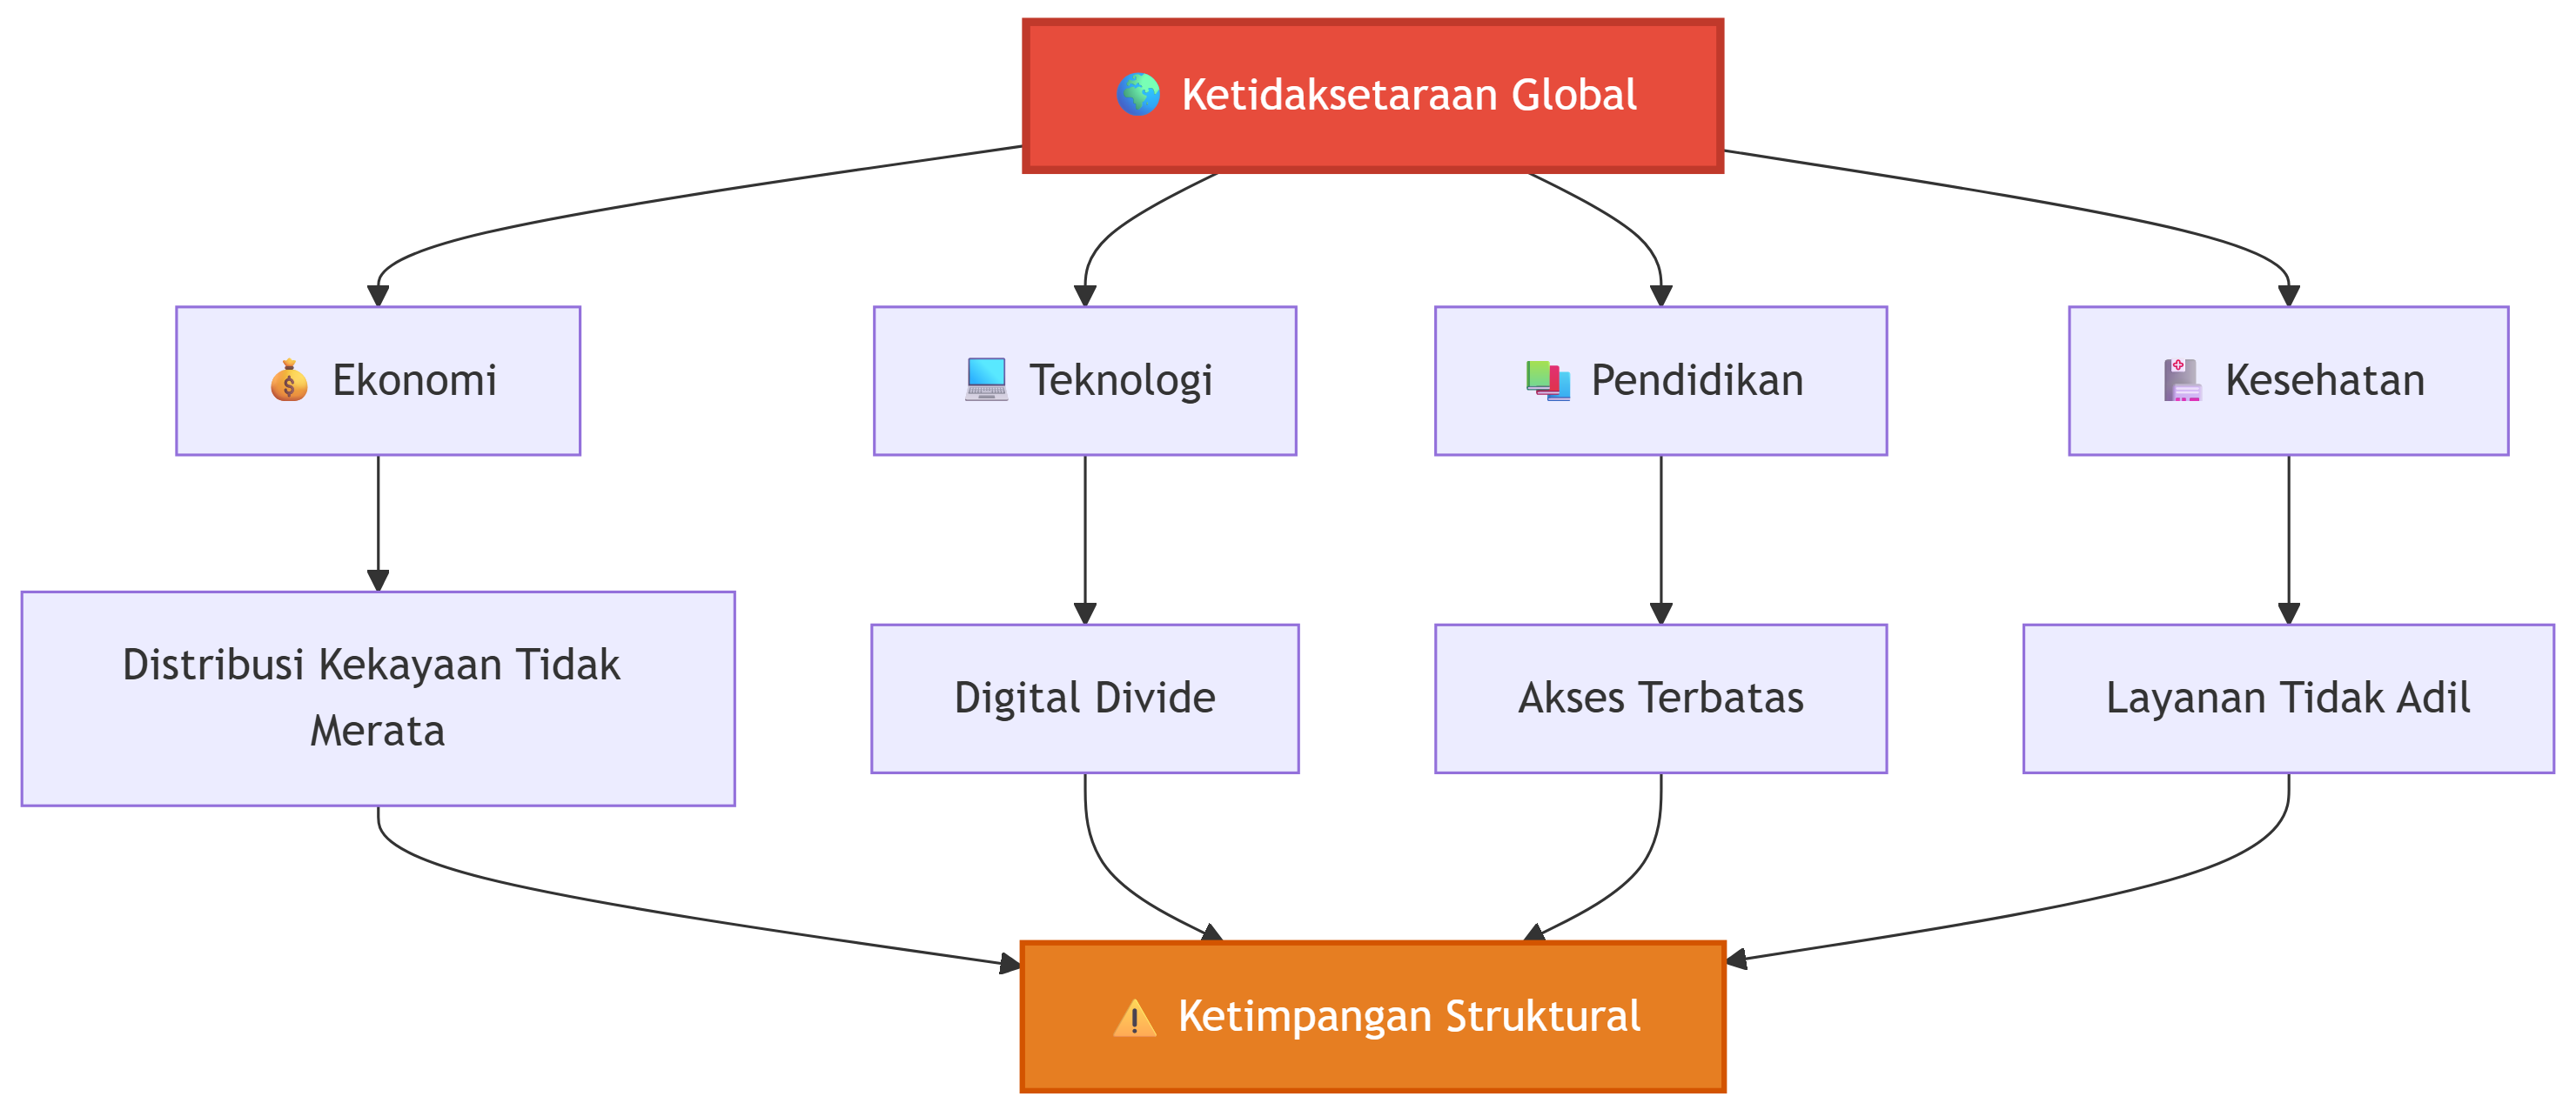
\includegraphics[width=9.79in,height=4.23in]{My_Concepts/index_files/figure-latex/mermaid-figure-1.png}

\subsection{Latar Belakang Masalah}\label{latar-belakang-masalah}

Ketidaksetaraan global merupakan kondisi di mana manfaat pertumbuhan
ekonomi, kemajuan teknologi, dan pembangunan sosial terdistribusi secara
timpang antara individu, kelompok sosial, maupun antarnegara. Meskipun
dunia memasuki era Artificial Intelligence (AI) dan transformasi digital
yang pesat, mayoritas populasi global belum merasakan manfaatnya secara
adil.

Ketimpangan ini tidak hanya muncul dalam bentuk perbedaan pendapatan dan
kekayaan, tetapi juga tercermin dalam akses terhadap pendidikan, layanan
kesehatan, teknologi informasi, dan peluang ekonomi. Ketidaksetaraan
yang ekstrem berkontribusi terhadap meningkatnya kemiskinan relatif,
melemahnya kohesi sosial, serta ketidakstabilan sosial-politik dalam
jangka panjang

\begin{center}\rule{0.5\linewidth}{0.5pt}\end{center}

\subsection{Definisi Konsep}\label{definisi-konsep}

\textbf{Ketidaksetaraan Global (Konsep)} dapat didefinisikan sebagai:

\begin{quote}
\textbf{Logika mesin abstrak} yang berusaha mengarahkan dan mengelola
\textbf{kekuatan sistem global {[}K{]}}\\
--- seperti teknologi, kebijakan, data, dan sumber daya ekonomi ---\\
untuk \textbf{mengangkat beban ketimpangan struktural {[}B{]}}\\
yang membatasi akses sebagian besar populasi dunia terhadap
kesejahteraan, peluang, dan martabat hidup yang setara.
\end{quote}

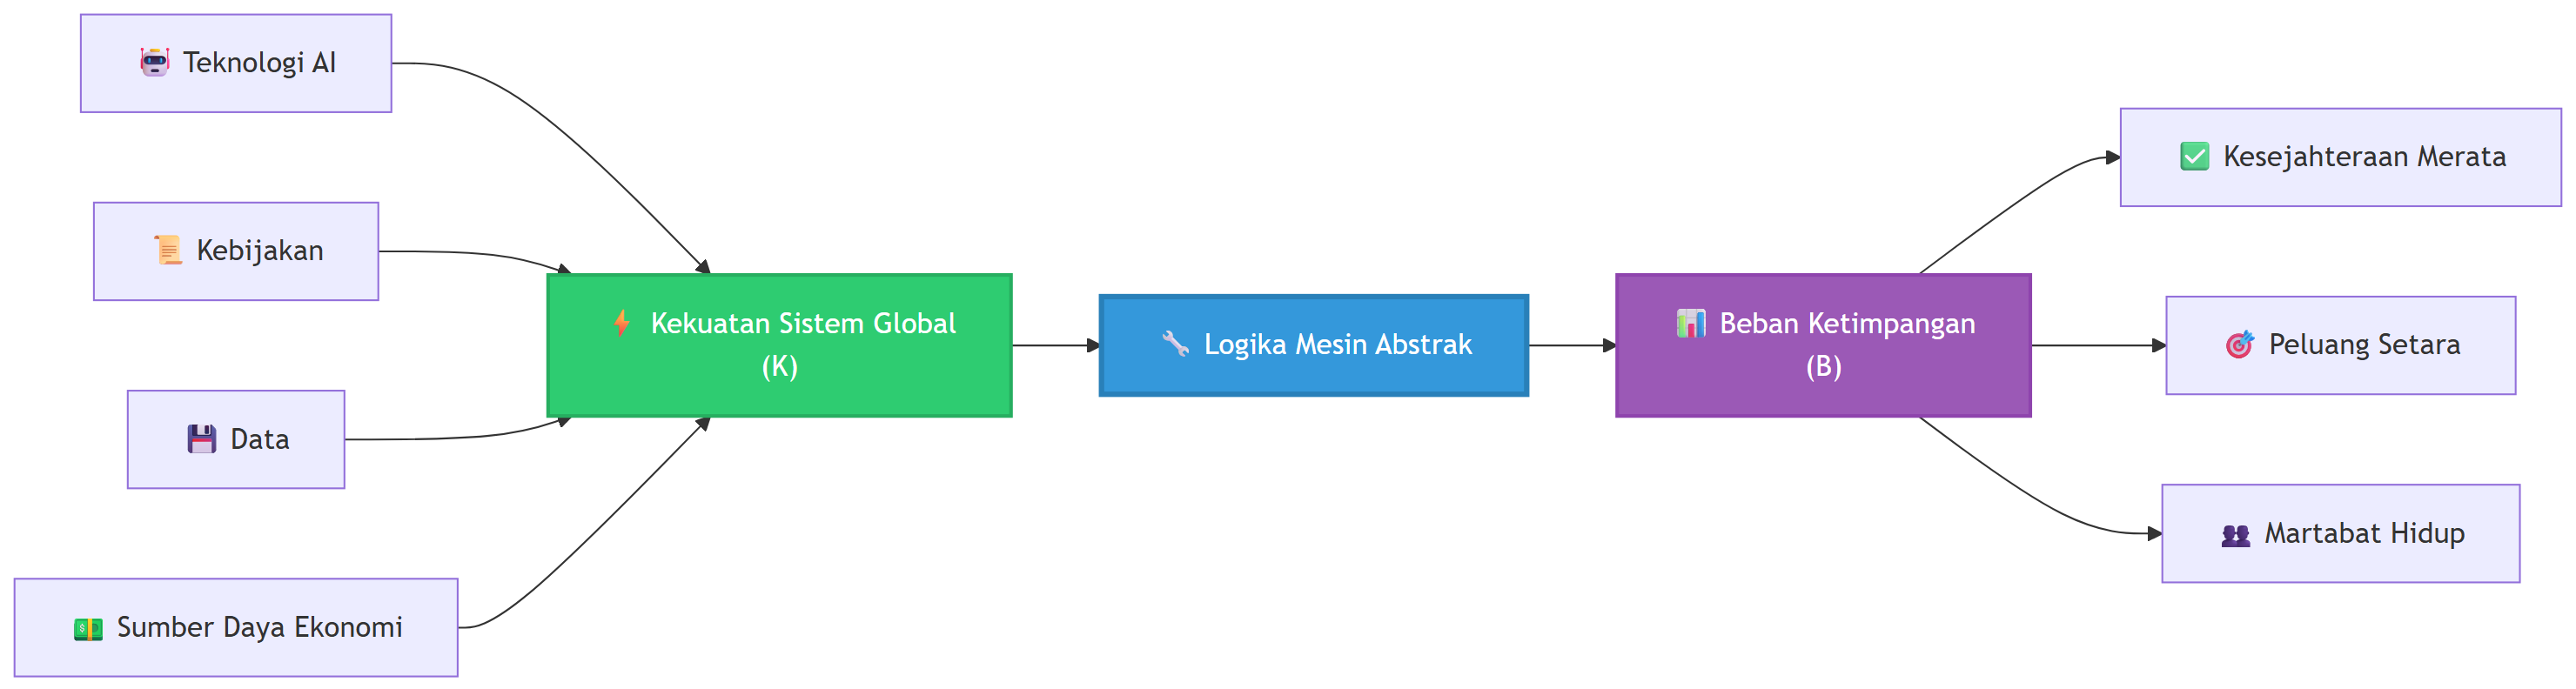
\includegraphics[width=14.83in,height=3.98in]{My_Concepts/index_files/figure-latex/mermaid-figure-4.png}

Konsep ini tidak bertujuan untuk menjelaskan seluruh detail fenomena
ketimpangan, melainkan menyaring esensi dari masalah:
\textbf{ketidakseimbangan distribusi manfaat kemajuan manusia}.

\begin{center}\rule{0.5\linewidth}{0.5pt}\end{center}

\subsection{Esensi Konsep (Inti
Pemikiran)}\label{esensi-konsep-inti-pemikiran}

Esensi dari konsep Ketidaksetaraan Global terletak pada tiga gagasan
utama:

\begin{enumerate}
\def\labelenumi{\arabic{enumi}.}
\item
  \textbf{Ketimpangan Bersifat Sistemik}\\
  Ketidaksetaraan bukan sekadar hasil kegagalan individu, melainkan
  konsekuensi dari sistem ekonomi, politik, dan teknologi global yang
  bekerja tidak seimbang.
\item
  \textbf{Teknologi Bersifat Ambivalen}\\
  Sistem dan teknologi informasi (termasuk AI) dapat menjadi alat
  pembebas atau justru memperdalam jurang ketimpangan, tergantung pada
  bagaimana ia dirancang, diakses, dan diatur.
\item
  \textbf{Distribusi Akses Lebih Penting dari Inovasi Semata}\\
  Inovasi tanpa pemerataan akses hanya akan mempercepat akumulasi
  keuntungan pada kelompok yang sudah diuntungkan sebelumnya.
\end{enumerate}

\begin{center}\rule{0.5\linewidth}{0.5pt}\end{center}

\subsection{Peran Konsep sebagai Induk
Ide}\label{peran-konsep-sebagai-induk-ide}

Sebagai sebuah konsep, Ketidaksetaraan Global berfungsi sebagai
\textbf{induk dari berbagai ide praktis}, antara lain:

\begin{itemize}
\tightlist
\item
  Sistem AI untuk pemerataan akses pendidikan dan literasi digital\\
\item
  Kebijakan berbasis data untuk redistribusi sumber daya secara lebih
  adil\\
\item
  Platform teknologi inklusif bagi negara berkembang dan kelompok
  marginal\\
\item
  Mekanisme pengukuran ketimpangan digital (digital divide) secara
  real-time
\end{itemize}

Setiap ide praktis tersebut mewarisi kualitas dari konsep induknya:
\textbf{keadilan, inklusivitas, dan keberlanjutan}.

\begin{center}\rule{0.5\linewidth}{0.5pt}\end{center}

\subsection{Konsep sebagai Persimpangan
Jalan}\label{konsep-sebagai-persimpangan-jalan}

\begin{figure}[H]

{\centering \pandocbounded{\includegraphics[keepaspectratio]{index_files/mediabag/photo-1473186578172-.jpg}}

}

\caption{Decision Path}

\end{figure}%

Konsep Ketidaksetaraan Global dapat dipandang sebagai
\textbf{persimpangan jalan pemikiran}, yang membuka berbagai arah
tindakan:

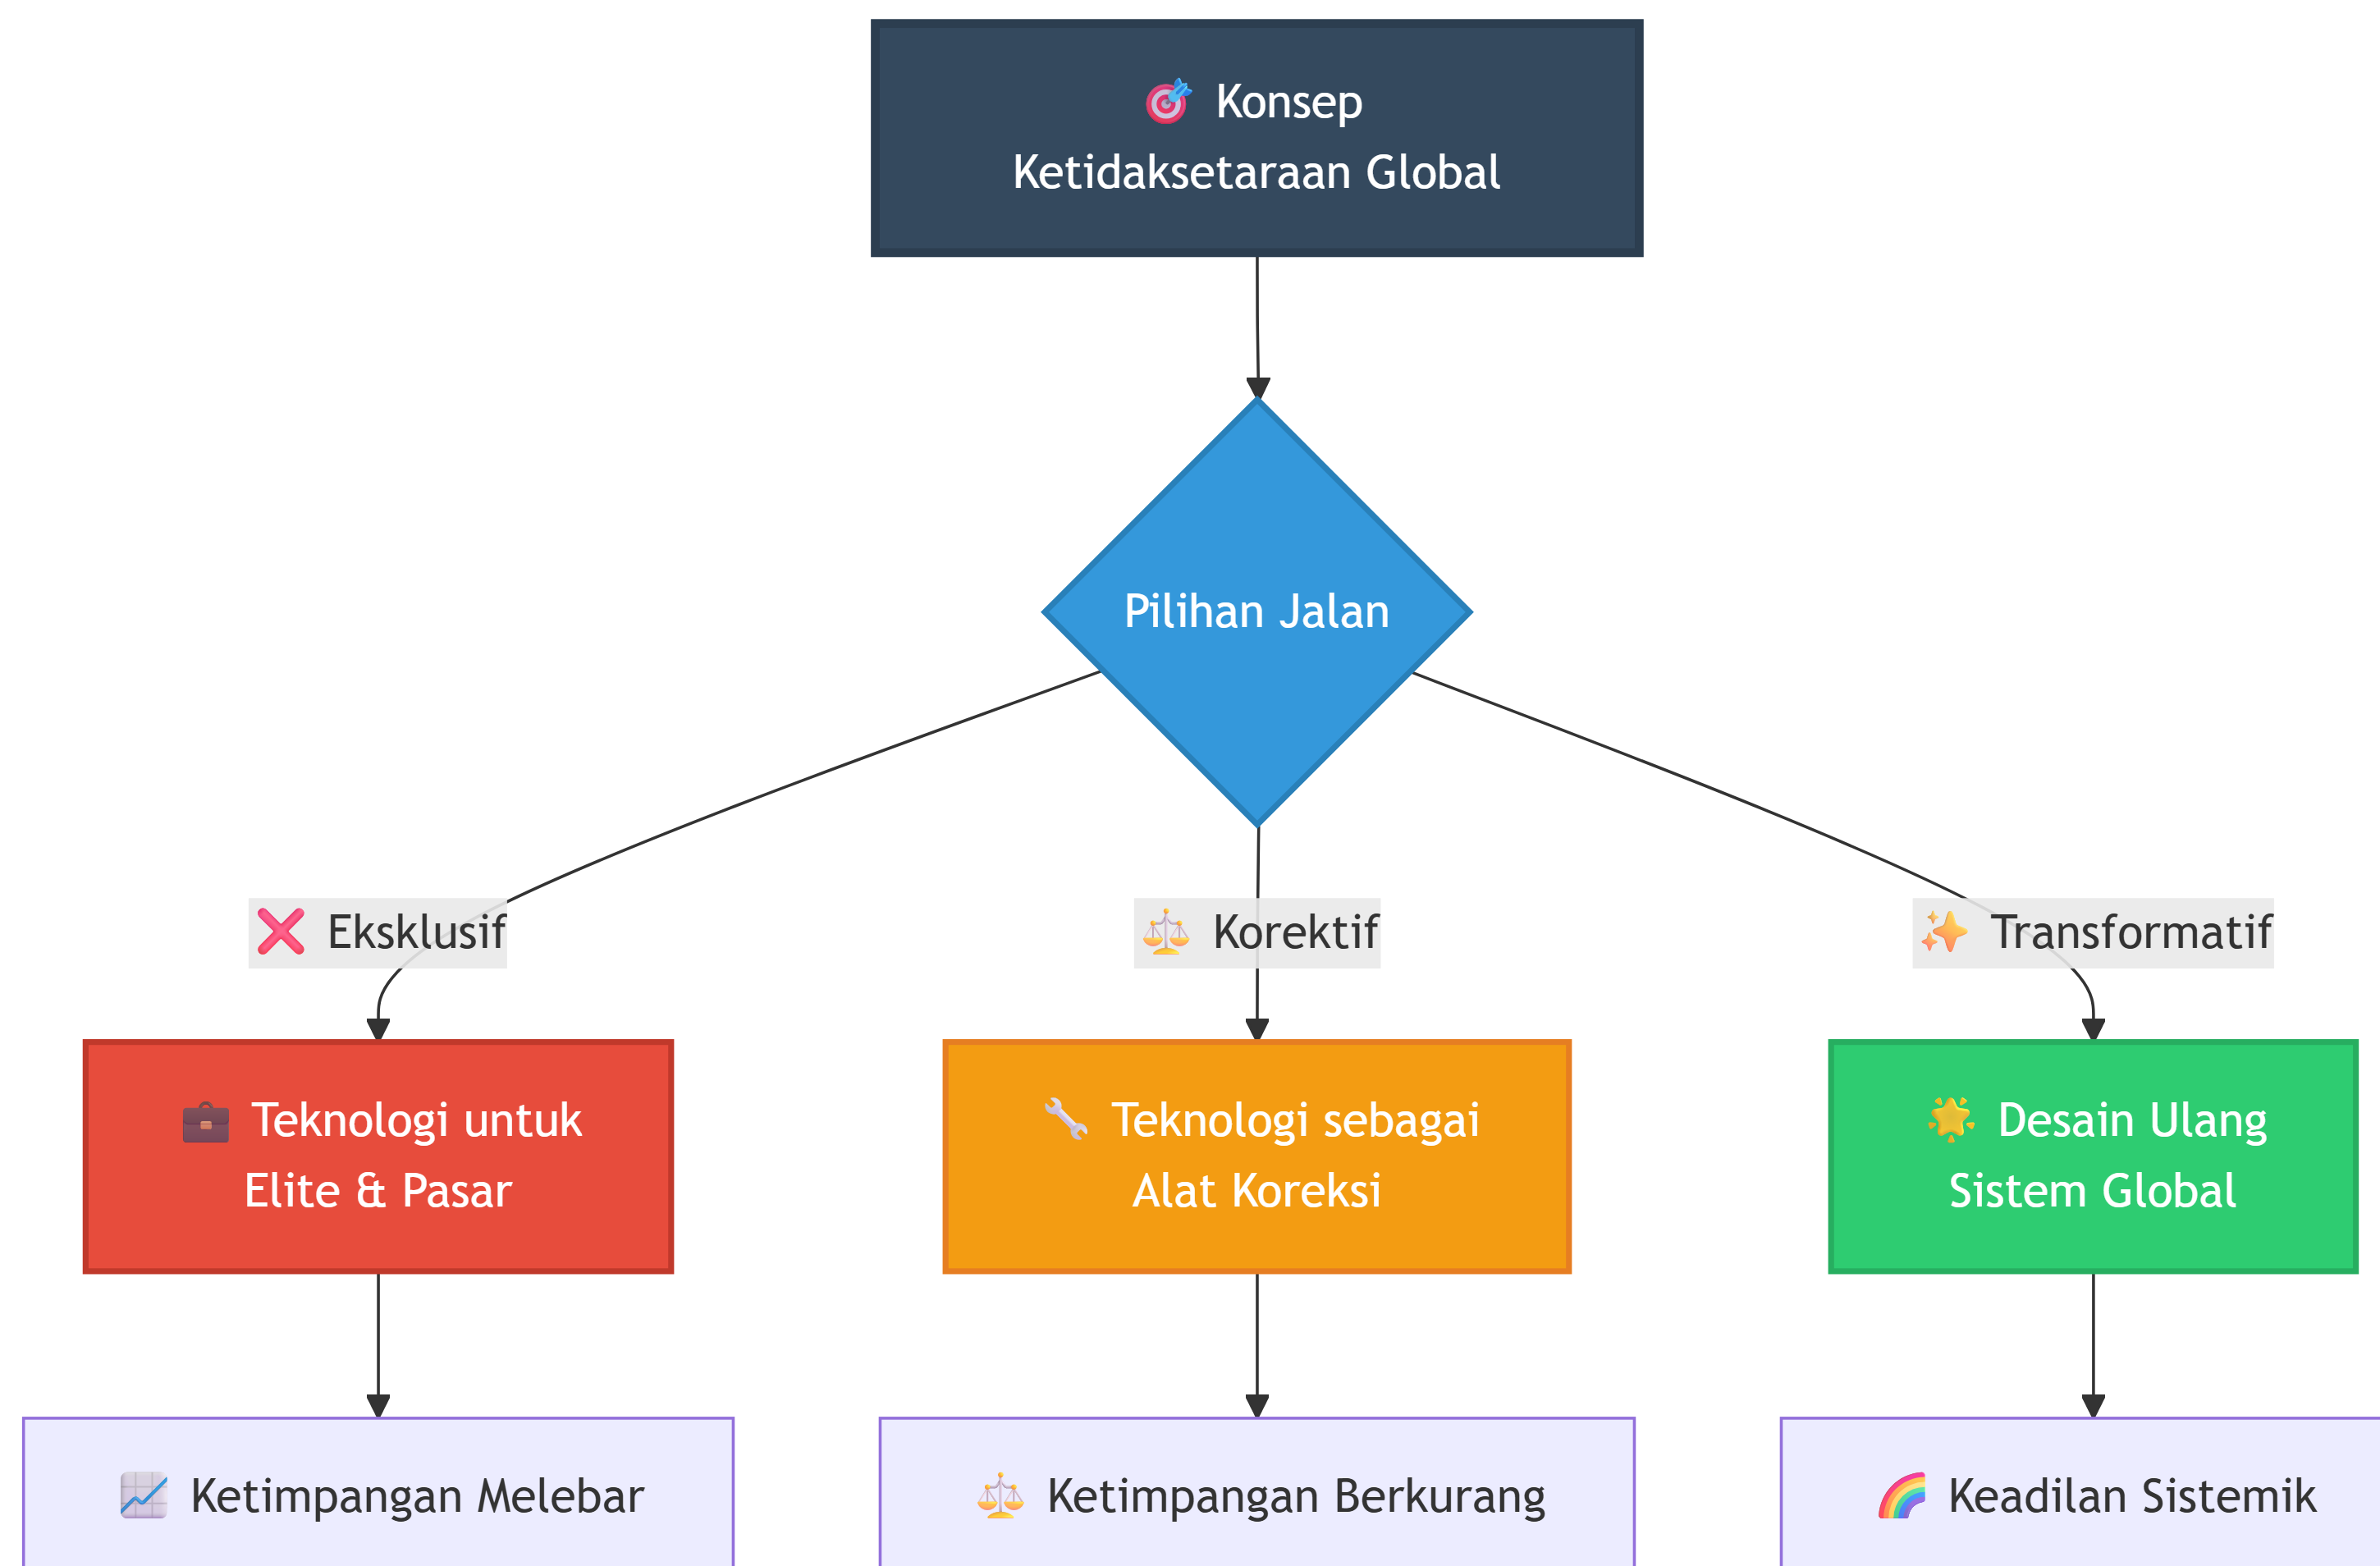
\includegraphics[width=8.61in,height=5.67in]{My_Concepts/index_files/figure-latex/mermaid-figure-3.png}

\begin{itemize}
\tightlist
\item
  \textbf{Jalan eksklusif:} teknologi hanya melayani pasar dan elite
  global\\
\item
  \textbf{Jalan korektif:} teknologi digunakan sebagai alat koreksi
  ketimpangan\\
\item
  \textbf{Jalan transformatif:} sistem global didesain ulang dengan
  keadilan sebagai prinsip utama
\end{itemize}

Konsep ini membantu memilih jalan mana yang akan ditempuh, terutama
dalam situasi di mana tidak ada rutinitas atau solusi siap pakai.

\begin{center}\rule{0.5\linewidth}{0.5pt}\end{center}

\subsection{Analogi untuk Memperjelas}\label{analogi-untuk-memperjelas}

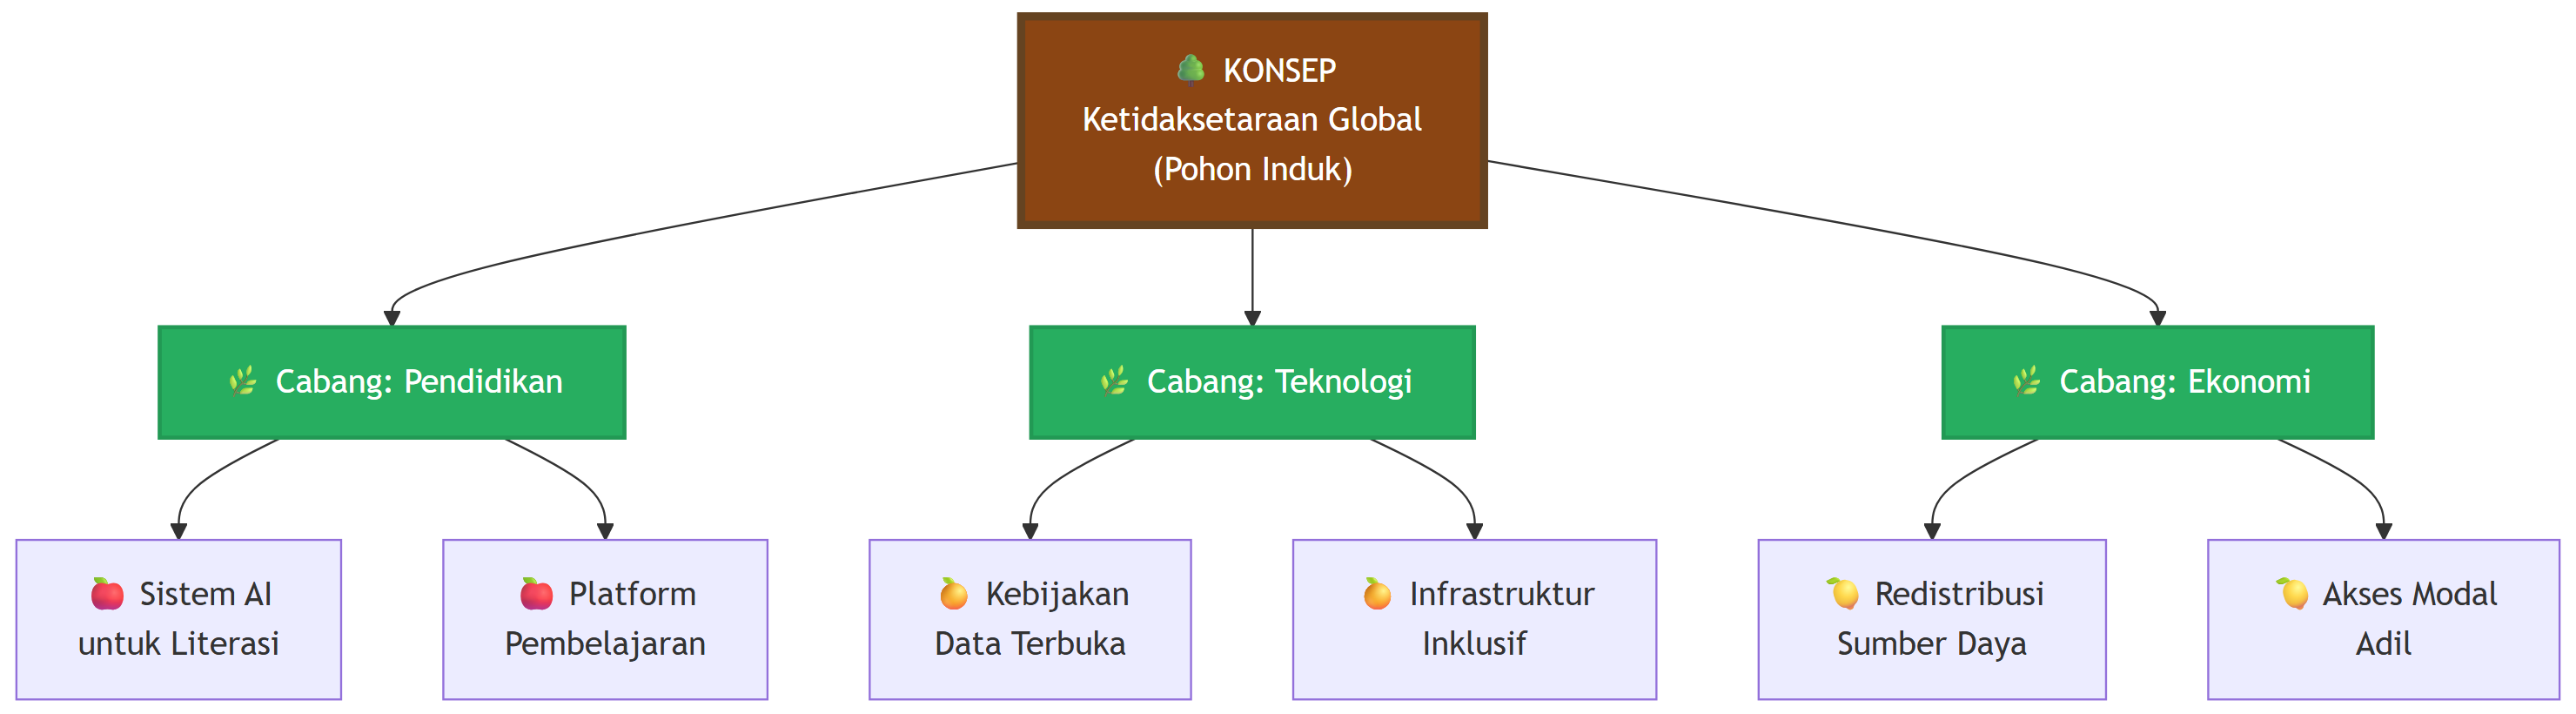
\includegraphics[width=13.13in,height=3.65in]{My_Concepts/index_files/figure-latex/mermaid-figure-2.png}

Jika \textbf{ide-ide praktis} adalah \emph{buah} seperti kebijakan,
aplikasi, atau sistem AI tertentu,\\
maka \textbf{konsep Ketidaksetaraan Global} adalah \emph{pohon induk}
yang:

\begin{itemize}
\tightlist
\item
  Menentukan jenis buah yang dapat tumbuh\\
\item
  Menjadi sumber berkelanjutan bagi lahirnya ide-ide baru\\
\item
  Perlu dirawat agar tidak menjadi sekadar angan-angan (wishful
  thinking)
\end{itemize}

Tanpa membangun konsep yang kuat, setiap solusi hanya akan menjadi buah
sesaat tanpa keberlanjutan.

\begin{center}\rule{0.5\linewidth}{0.5pt}\end{center}

\subsection{Penutup}\label{penutup}

Dalam era Artificial Intelligence, ketidaksetaraan global bukan sekadar
masalah ekonomi, melainkan ujian moral dan sistemik bagi peradaban
manusia. Dengan memahami dan membangun konsep Ketidaksetaraan Global
secara sadar, kita menciptakan fondasi berpikir yang memungkinkan
lahirnya ide-ide praktis yang tidak hanya cerdas, tetapi juga adil dan
manusiawi.

Konsep ini menjadi langkah awal menuju \textbf{pikiran yang indah
(beautiful mind)}---pikiran yang mampu melihat esensi, bukan hanya
gejala.

\bookmarksetup{startatroot}

\chapter{UAS-2 My Opinions}\label{uas-2-my-opinions}

\begin{figure}[H]

{\centering \pandocbounded{\includegraphics[keepaspectratio]{index_files/mediabag/giphy1.gif}}

}

\caption{Perspective}

\end{figure}%

\section{Ketidaksetaraan Global di Era Artificial
Intelligence}\label{ketidaksetaraan-global-di-era-artificial-intelligence}

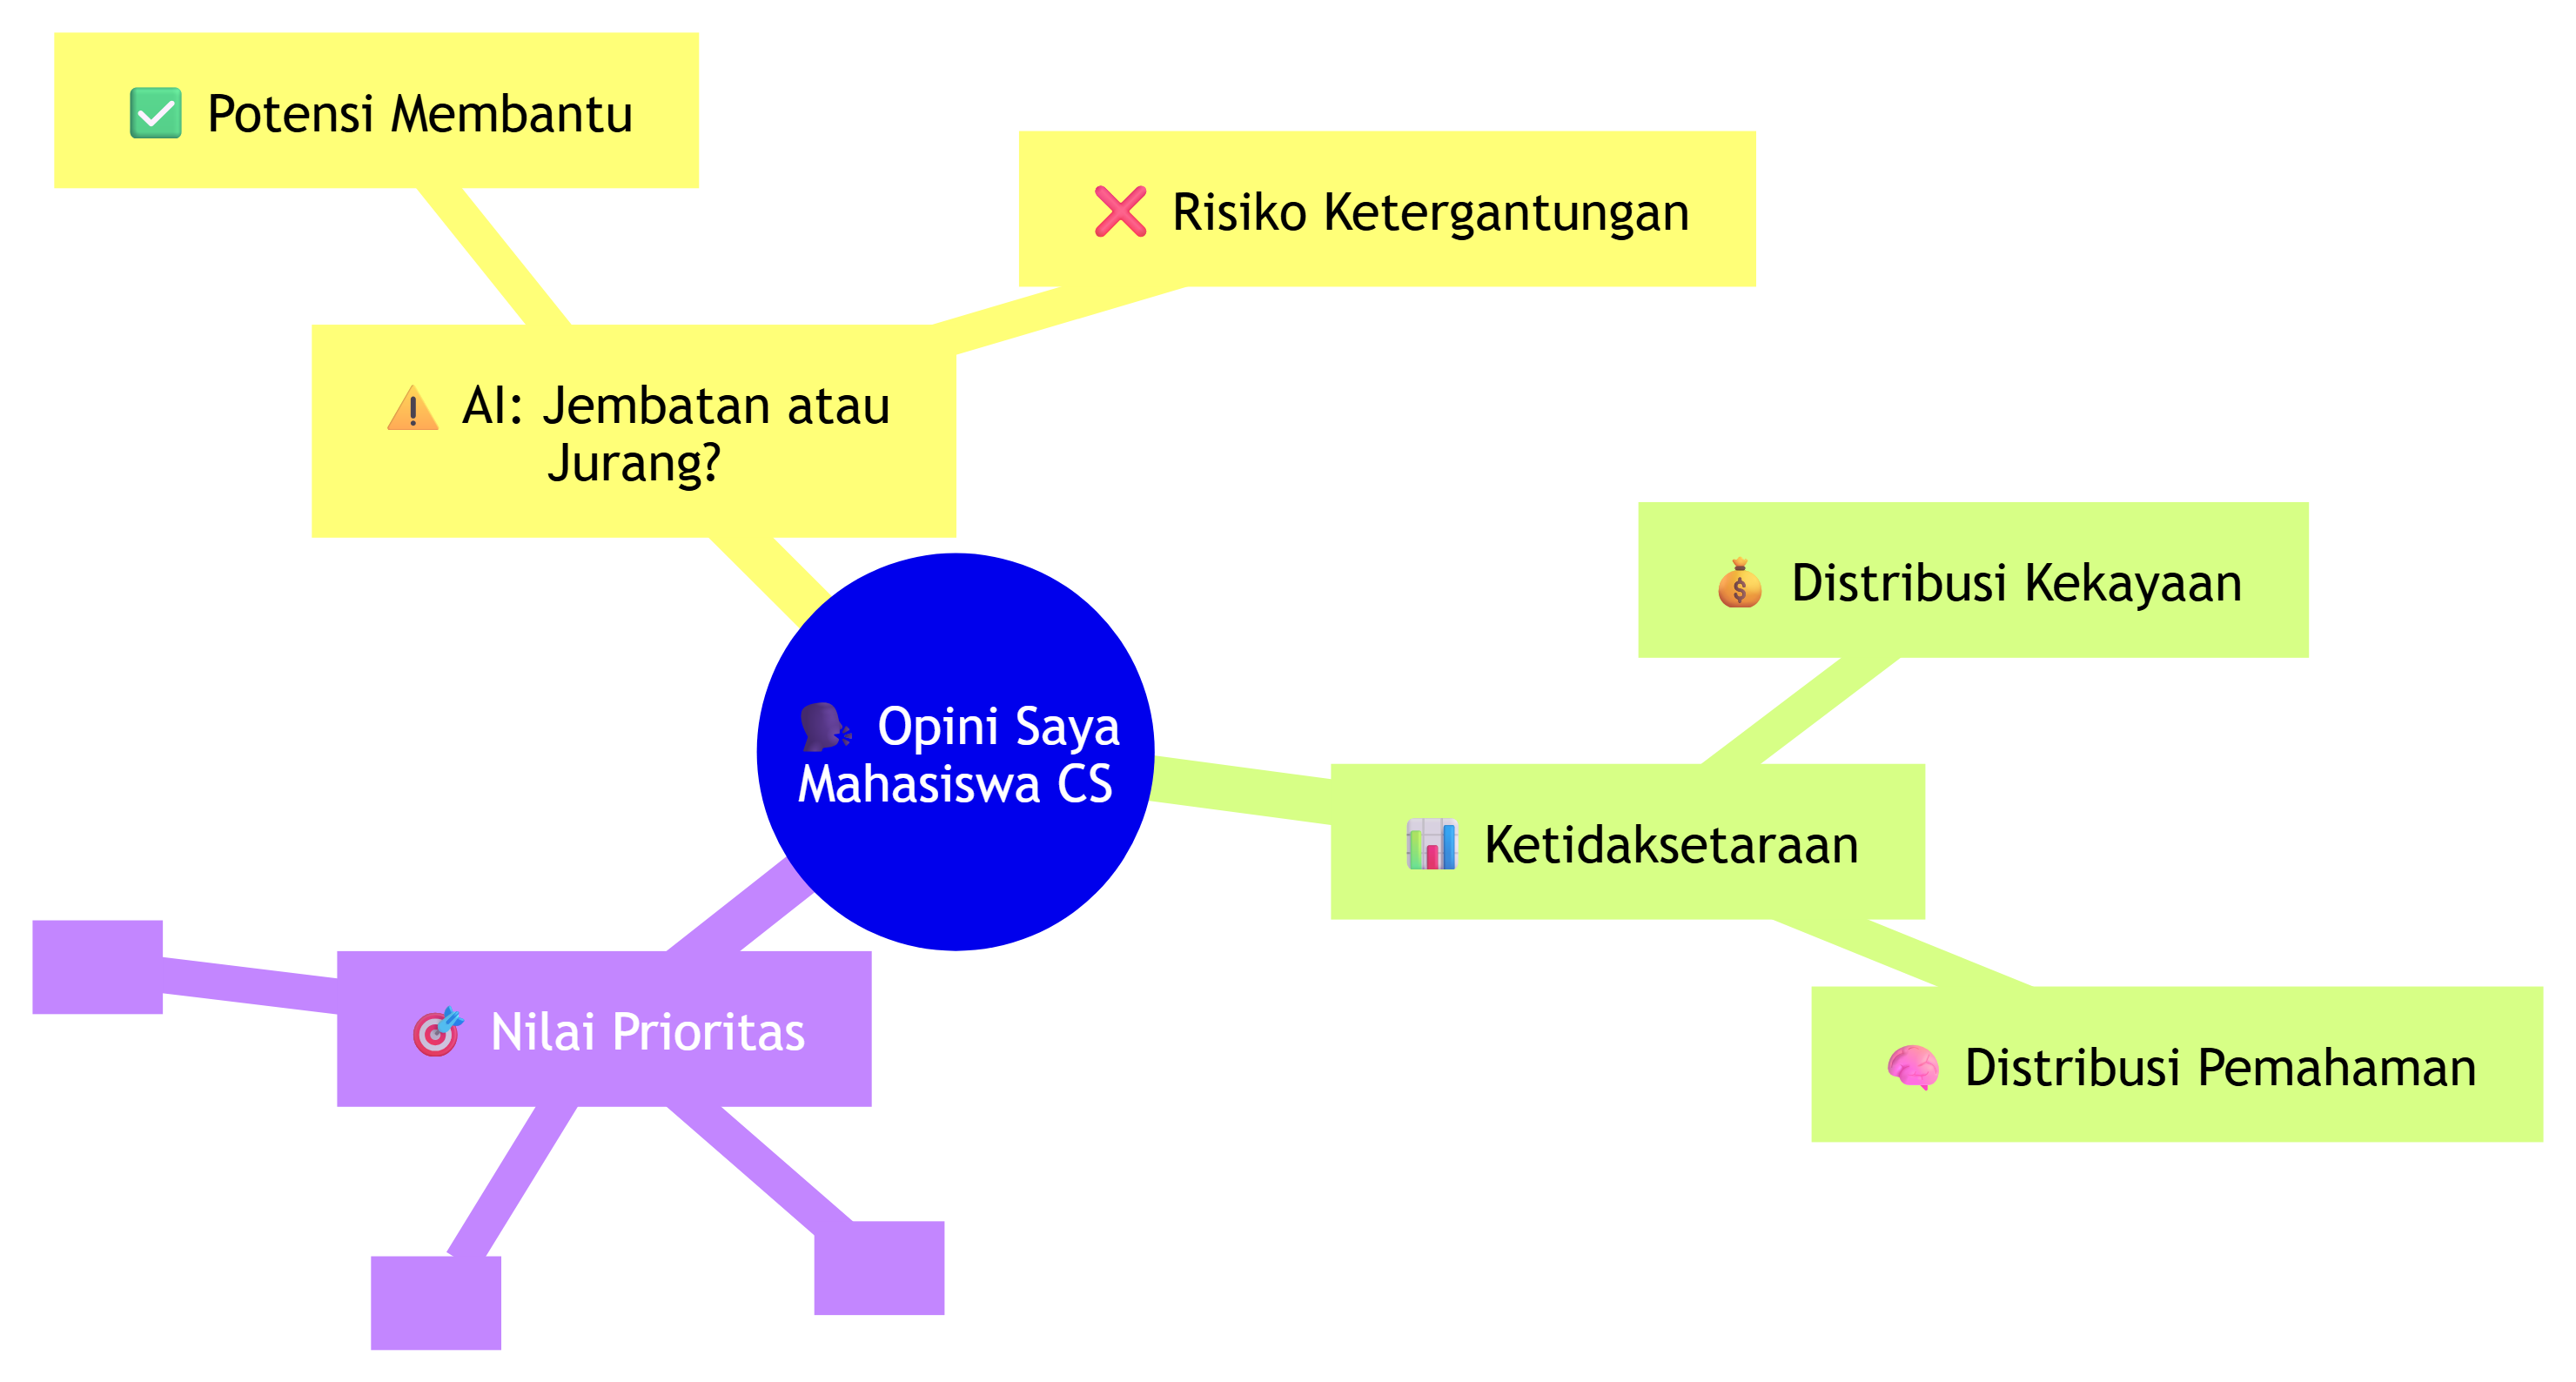
\includegraphics[width=8.24in,height=4.42in]{My_Opinions/index_files/figure-latex/mermaid-figure-1.png}

\subsection{Sudut Pandang Saya}\label{sudut-pandang-saya}

Opini ini saya sampaikan dari sudut pandang \textbf{seorang mahasiswa
Bachelor of Computer Science} yang hidup di era digital dan banyak
mengamati kondisi dunia melalui \textbf{media sosial}. Ini adalah
\textbf{opini pribadi}, namun saya percaya bahwa pandangan ini memiliki
relevansi yang lebih luas ketika membahas penerapan sistem dan teknologi
informasi di era Artificial Intelligence (AI).

\begin{center}\rule{0.5\linewidth}{0.5pt}\end{center}

\subsection{Opini Inti}\label{opini-inti}

\textbf{Saya percaya bahwa Artificial Intelligence memiliki potensi
besar untuk membantu mengatasi ketidaksetaraan global.}\\
Namun, saya juga meyakini bahwa \textbf{ketergantungan berlebihan
terhadap AI justru berisiko menciptakan bentuk ketidaksetaraan global
yang baru}---masalah lama yang berganti wajah.

Dengan kata lain, AI adalah alat yang berada di persimpangan: ia bisa
menjadi jembatan, atau justru jurang.

\begin{center}\rule{0.5\linewidth}{0.5pt}\end{center}

\subsection{Informasi yang Membentuk Pandangan
Saya}\label{informasi-yang-membentuk-pandangan-saya}

Ketidaksetaraan global, menurut saya, sangat terlihat dari
\textbf{distribusi kekayaan dan pemahaman}. Bukan hanya soal siapa yang
memiliki uang atau teknologi, tetapi siapa yang \textbf{memahami,
mengendalikan, dan mendapatkan manfaat terbesar} dari sistem yang
dibangun.

Dalam konteks AI, di satu sisi teknologi ini tampak inklusif---banyak
sistem AI dapat diakses oleh hampir semua orang. Namun di sisi lain,
\textbf{AI menuntut komputasi yang sangat mahal}, infrastruktur besar,
dan modal yang tidak kecil. Hal ini secara alami menguntungkan
perusahaan besar dan negara maju, sekaligus memperlebar jurang dengan
individu atau kelompok yang tidak memiliki sumber daya serupa.

\begin{center}\rule{0.5\linewidth}{0.5pt}\end{center}

\subsection{Nilai-Nilai yang Saya
Pegang}\label{nilai-nilai-yang-saya-pegang}

Dalam menilai peran AI terhadap ketidaksetaraan global, saya menempatkan
nilai-nilai berikut sebagai prioritas:

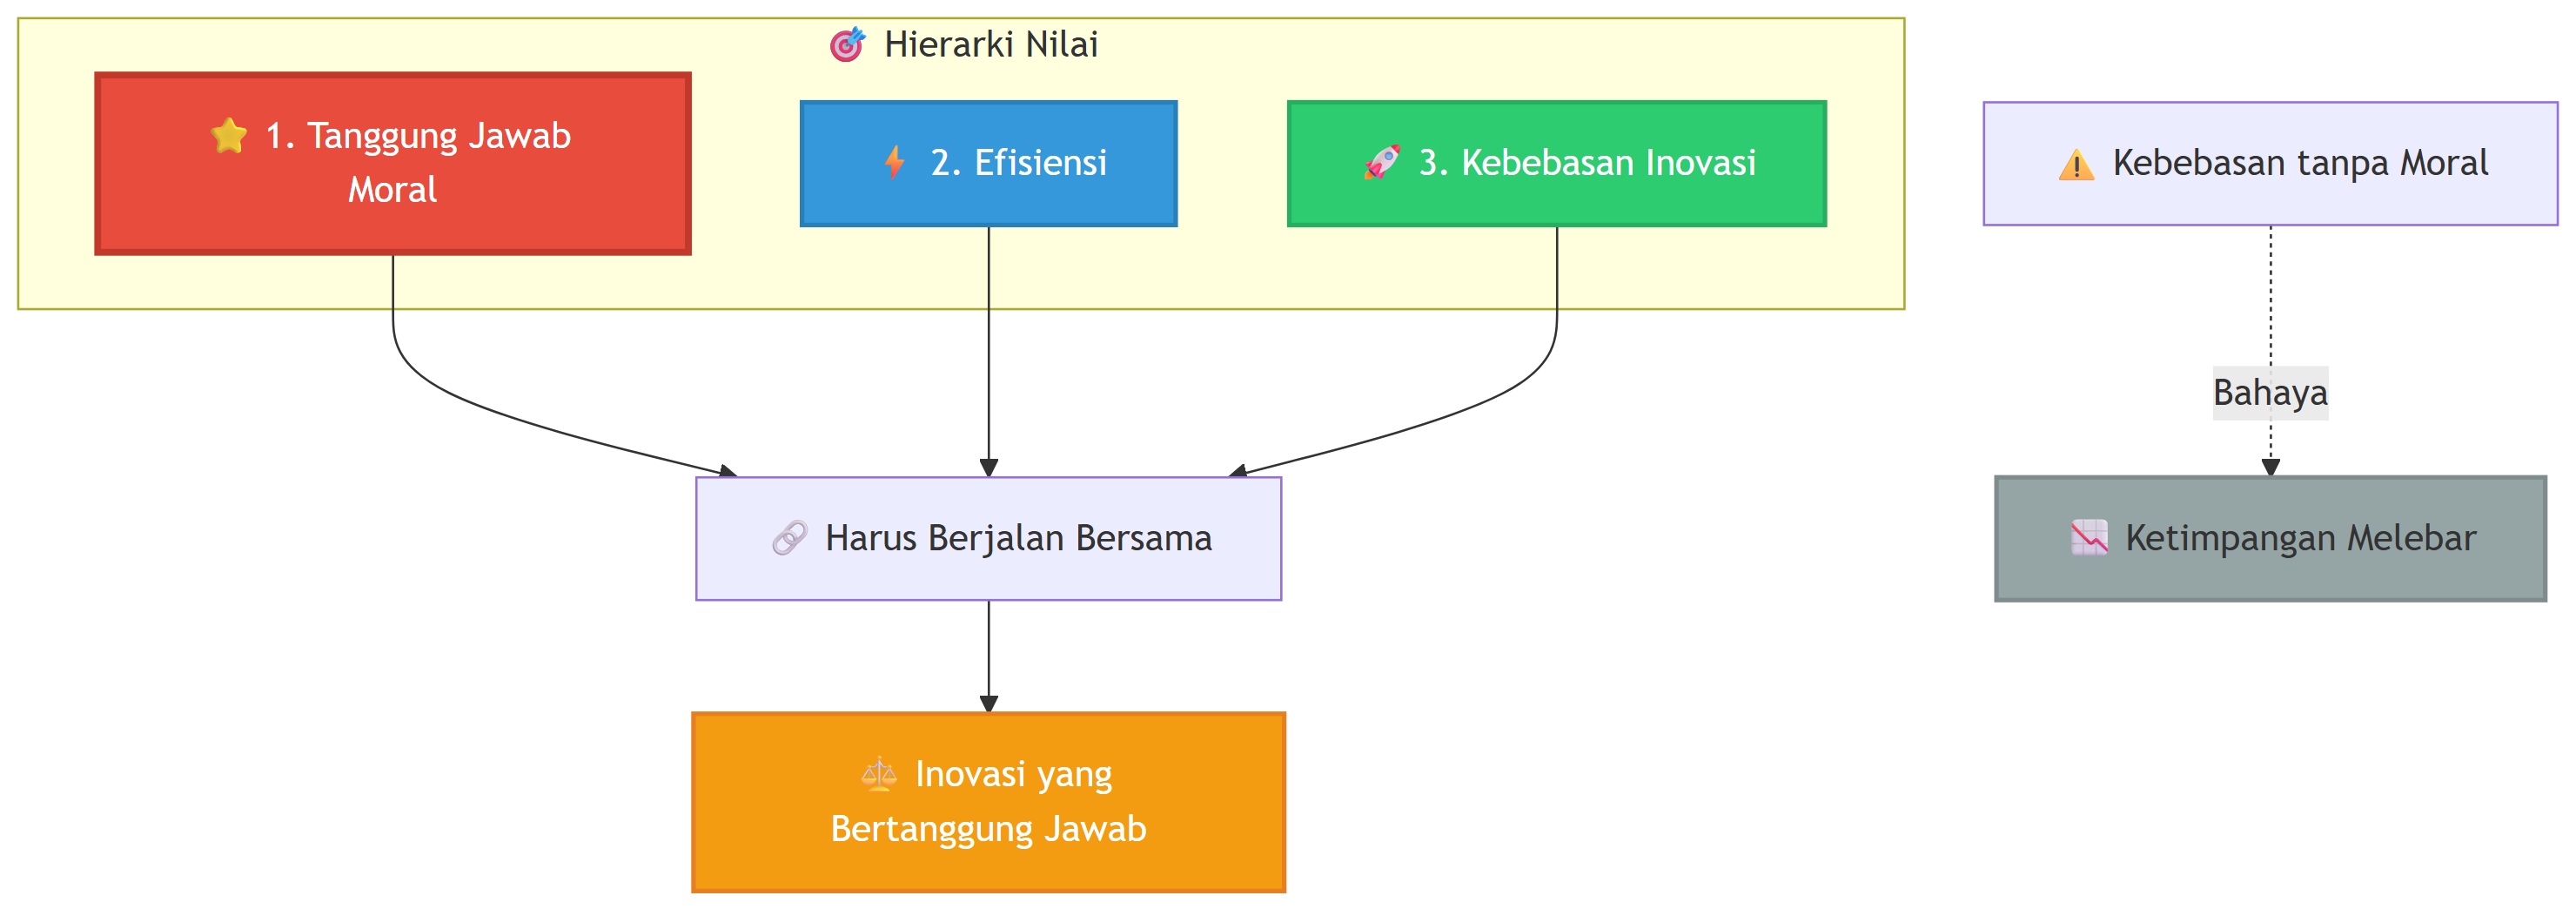
\includegraphics[width=11.81in,height=4.17in]{My_Opinions/index_files/figure-latex/mermaid-figure-5.png}

\begin{enumerate}
\def\labelenumi{\arabic{enumi}.}
\tightlist
\item
  \textbf{Tanggung jawab moral}\\
\item
  \textbf{Efisiensi}\\
\item
  \textbf{Kebebasan inovasi}
\end{enumerate}

Bagi saya, kebebasan inovasi tidak boleh berdiri tanpa tanggung jawab
moral. Inovasi yang efisien tetapi mengorbankan keadilan hanya akan
mempercepat ketimpangan, bukan menyelesaikannya.

\begin{center}\rule{0.5\linewidth}{0.5pt}\end{center}

\subsection{Inovasi: Cepat atau
Inklusif?}\label{inovasi-cepat-atau-inklusif}

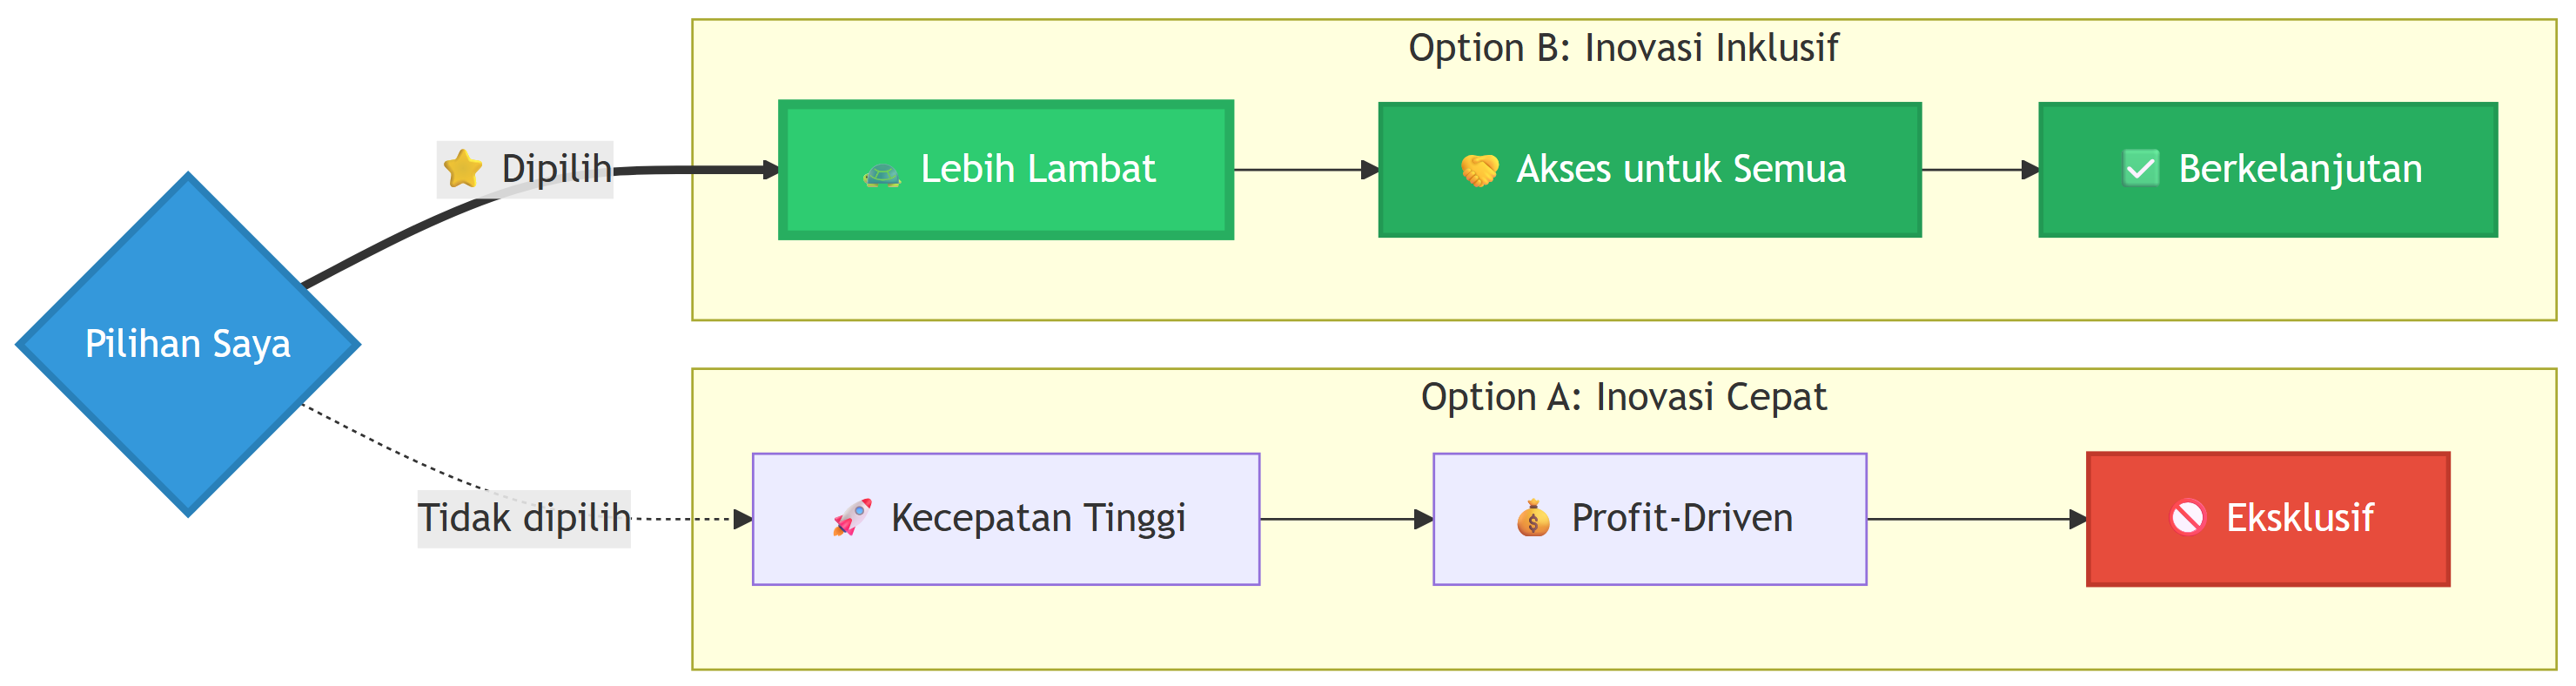
\includegraphics[width=11.06in,height=2.96in]{My_Opinions/index_files/figure-latex/mermaid-figure-4.png}

Saya lebih memilih \textbf{inovasi yang lebih lambat tetapi inklusif}.\\
Ironisnya, banyak Large Language Model (LLM) dan sistem AI awalnya
dikembangkan untuk meningkatkan aksesibilitas. Namun karena logika
profit, fokus tersebut bergeser ke pasar mayoritas yang paling
menguntungkan.

Menurut saya, \textbf{AI seharusnya bisa kembali berfokus pada
aksesibilitas dan kelompok inklusif}, bukan hanya pada skala dan
keuntungan.

\begin{center}\rule{0.5\linewidth}{0.5pt}\end{center}

\subsection{Perasaan dan Intuisi
Pribadi}\label{perasaan-dan-intuisi-pribadi}

\begin{figure}[H]

{\centering \pandocbounded{\includegraphics[keepaspectratio]{index_files/mediabag/photo-1516534775068-.jpg}}

}

\caption{Emotions}

\end{figure}%

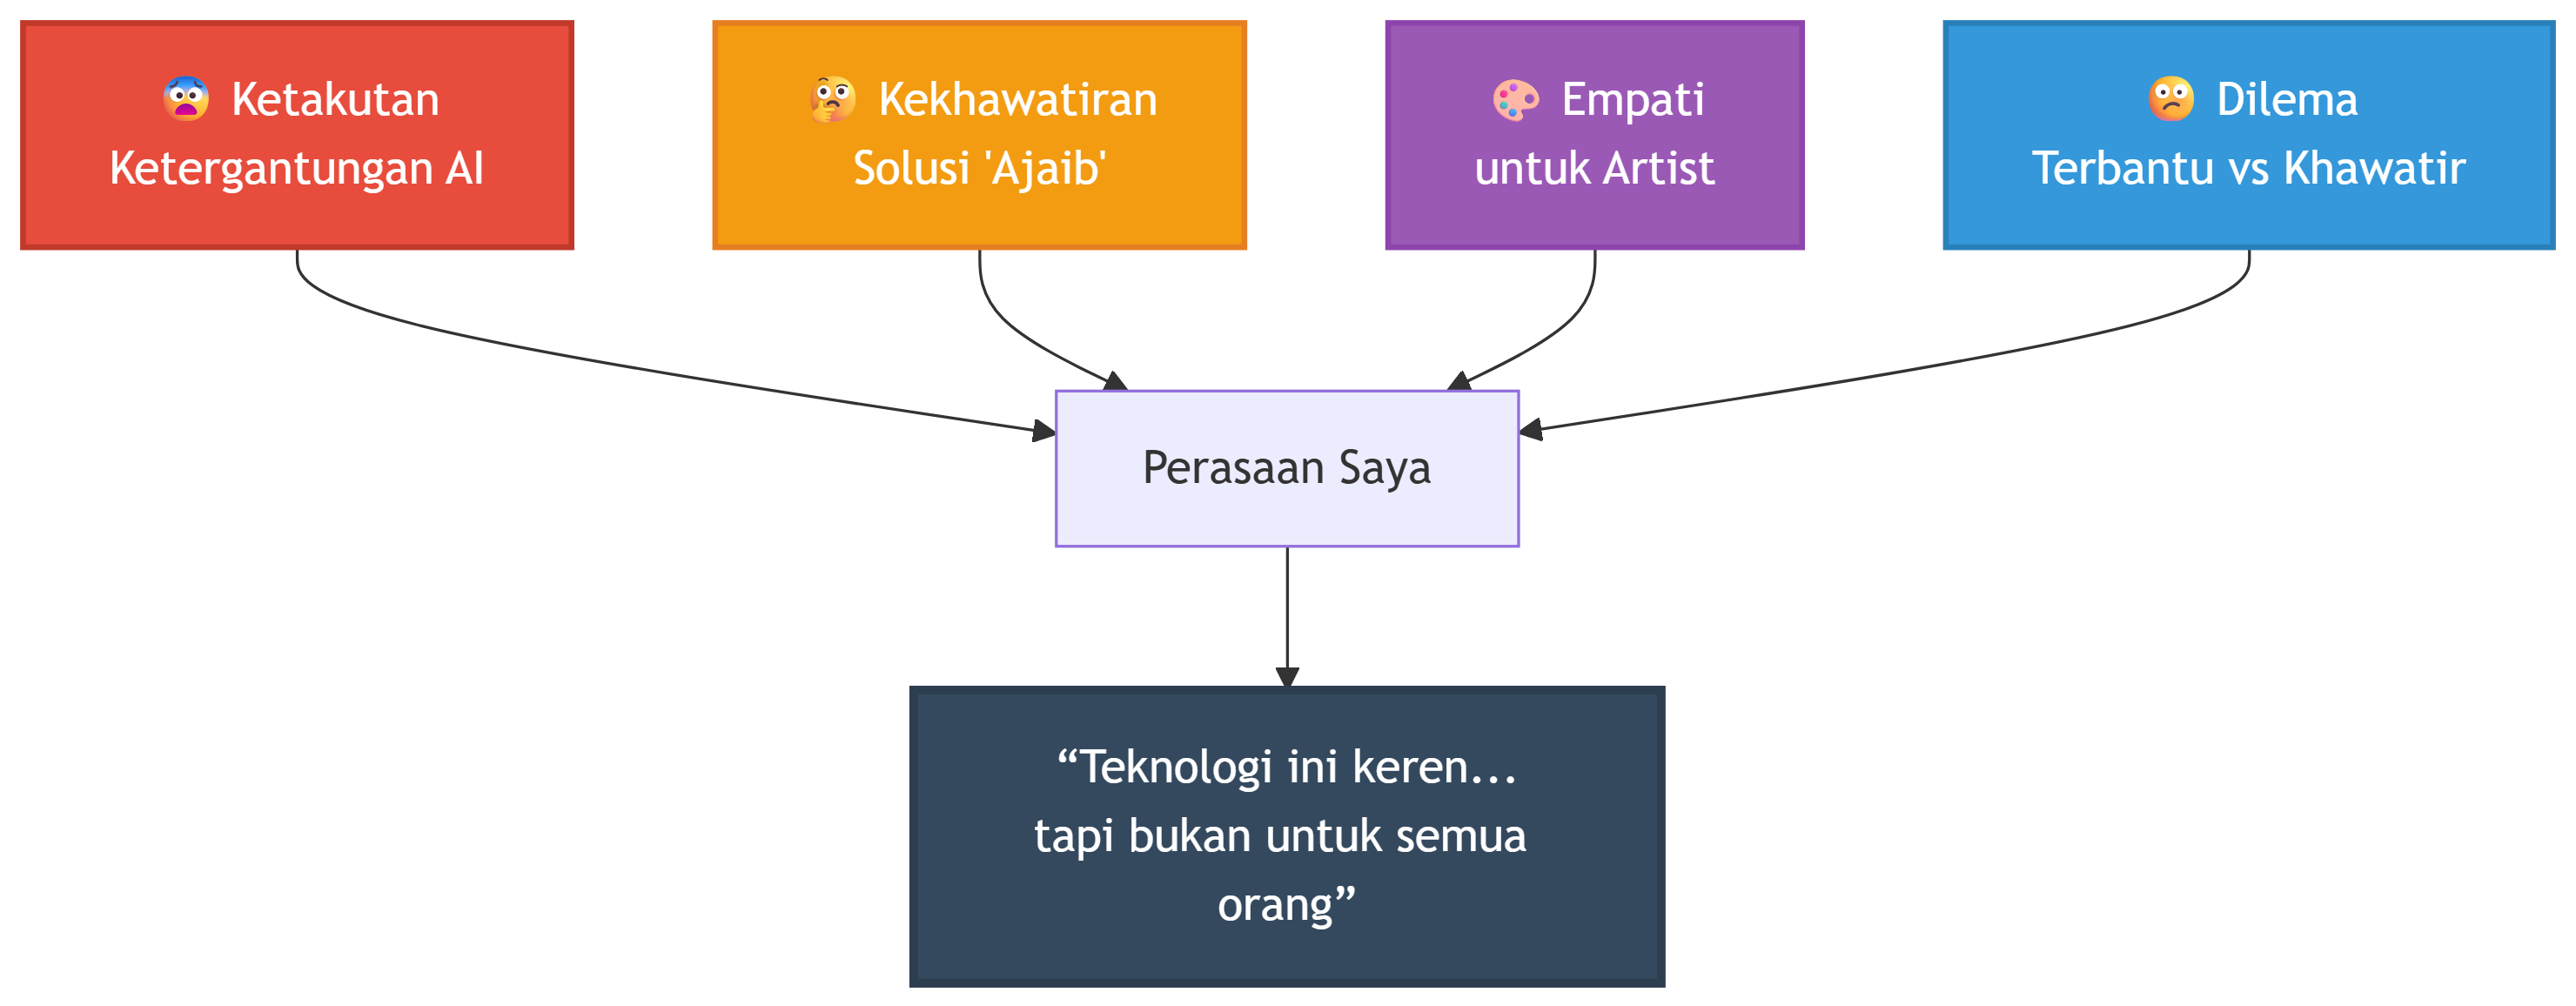
\includegraphics[width=9.33in,height=3.65in]{My_Opinions/index_files/figure-latex/mermaid-figure-3.png}

Secara emosional, yang paling saya rasakan adalah \textbf{ketakutan
terhadap ketergantungan manusia pada AI}.\\
Ada kekhawatiran bahwa manusia mulai memperlakukan AI sebagai solusi
``ajaib'' untuk segala hal---padahal tidak semua masalah bersifat
teknis.

Saya sering merasa:

\begin{quote}
\emph{``Teknologi ini memang keren\ldots{} tapi sepertinya bukan untuk
semua orang.''}
\end{quote}

Perasaan ini sangat terasa dalam dunia seni, khususnya bagi para artist,
di mana karya mereka diambil dan digunakan sebagai data pelatihan AI
tanpa pengetahuan atau izin. Dalam konteks ini, AI tidak terasa
inklusif, melainkan eksploitatif.

\begin{center}\rule{0.5\linewidth}{0.5pt}\end{center}

\subsection{Pengalaman Pribadi}\label{pengalaman-pribadi}

Dari pengalaman saya sendiri, ketidaksetaraan dalam AI paling jelas
terlihat dari fakta bahwa \textbf{perusahaan besar jauh lebih
diuntungkan dibandingkan individu biasa}.\\
Padahal, menurut saya, idealnya justru sebaliknya: teknologi seharusnya
memperkuat individu, bukan hanya institusi besar.

Saya merasa \textbf{beruntung dan terbantu} oleh AI, tetapi pada saat
yang sama, saya berharap bahwa \textbf{``AI bubble'' suatu saat akan
meledak}---bukan untuk menghancurkan AI, melainkan untuk mengoreksi arah
dan ekspektasi yang terlalu berlebihan.

\begin{center}\rule{0.5\linewidth}{0.5pt}\end{center}

\subsection{Peran Ideal AI Menurut
Saya}\label{peran-ideal-ai-menurut-saya}

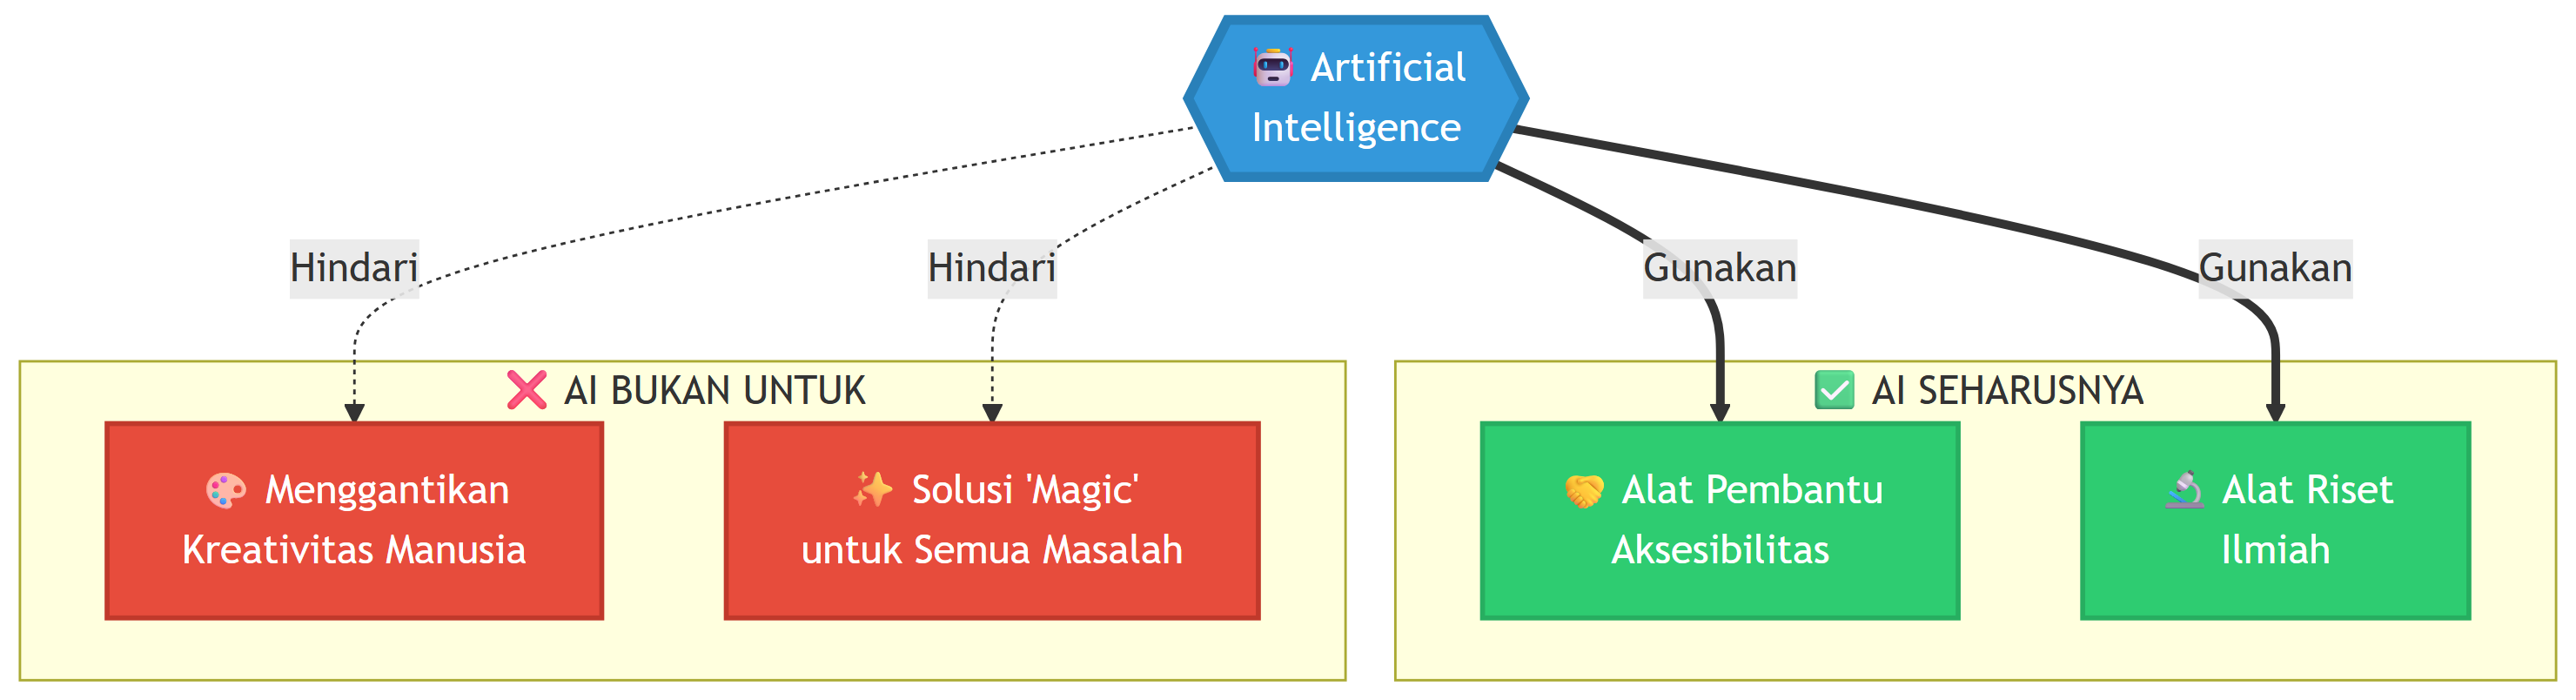
\includegraphics[width=10.77in,height=2.93in]{My_Opinions/index_files/figure-latex/mermaid-figure-2.png}

Menurut saya, AI seharusnya berperan sebagai:

\begin{itemize}
\tightlist
\item
  \textbf{Alat pembantu}, terutama dalam hal aksesibilitas\\
\item
  \textbf{Alat riset ilmiah}, dengan tujuan objektif untuk kemajuan
  manusia
\end{itemize}

AI \textbf{bukan} alat untuk: - Menggantikan kreativitas dan jiwa seni
manusia\\
- Menjadi solusi ``magic'' yang menghapus kompleksitas masalah sosial

\begin{center}\rule{0.5\linewidth}{0.5pt}\end{center}

\subsection{Kesiapan Mengubah Opini}\label{kesiapan-mengubah-opini}

Saya terbuka untuk mengubah atau merevisi opini ini di masa depan,
\textbf{jika terdapat dampak nyata} yang menunjukkan bahwa AI
benar-benar mampu mengurangi ketidaksetaraan secara sistemik dan
berkelanjutan.

Saya lebih takut \textbf{tidak memiliki opini sama sekali} daripada
memiliki opini yang salah. Manusia diciptakan dengan ego dan kebutuhan
untuk didengar. Bagi saya, beropini adalah bagian dari menjadi
manusia---selama kita siap merevisinya.

\begin{center}\rule{0.5\linewidth}{0.5pt}\end{center}

\subsection{Penutup: Harapan Saya}\label{penutup-harapan-saya}

Harapan saya terhadap masa depan ketidaksetaraan global di era AI adalah
sederhana namun berat:

\begin{quote}
\textbf{Semoga AI tidak hanya menjadi simbol kecanggihan,\\
tetapi juga bukti bahwa manusia masih mampu memilih keadilan\\
di tengah efisiensi dan kekuatan teknologi.}
\end{quote}

Opini ini bukan kesimpulan akhir, melainkan bagian dari proses berpikir
menuju \emph{beautiful mind}---pikiran yang berani bersuara, namun tetap
siap berubah.

\bookmarksetup{startatroot}

\chapter{UAS-3 My Knowledge}\label{uas-3-my-knowledge}

\begin{figure}[H]

{\centering \pandocbounded{\includegraphics[keepaspectratio]{index_files/mediabag/giphy12.gif}}

}

\caption{Study}

\end{figure}%

\section{Ketidaksetaraan Global di Era Artificial
Intelligence}\label{ketidaksetaraan-global-di-era-artificial-intelligence-1}

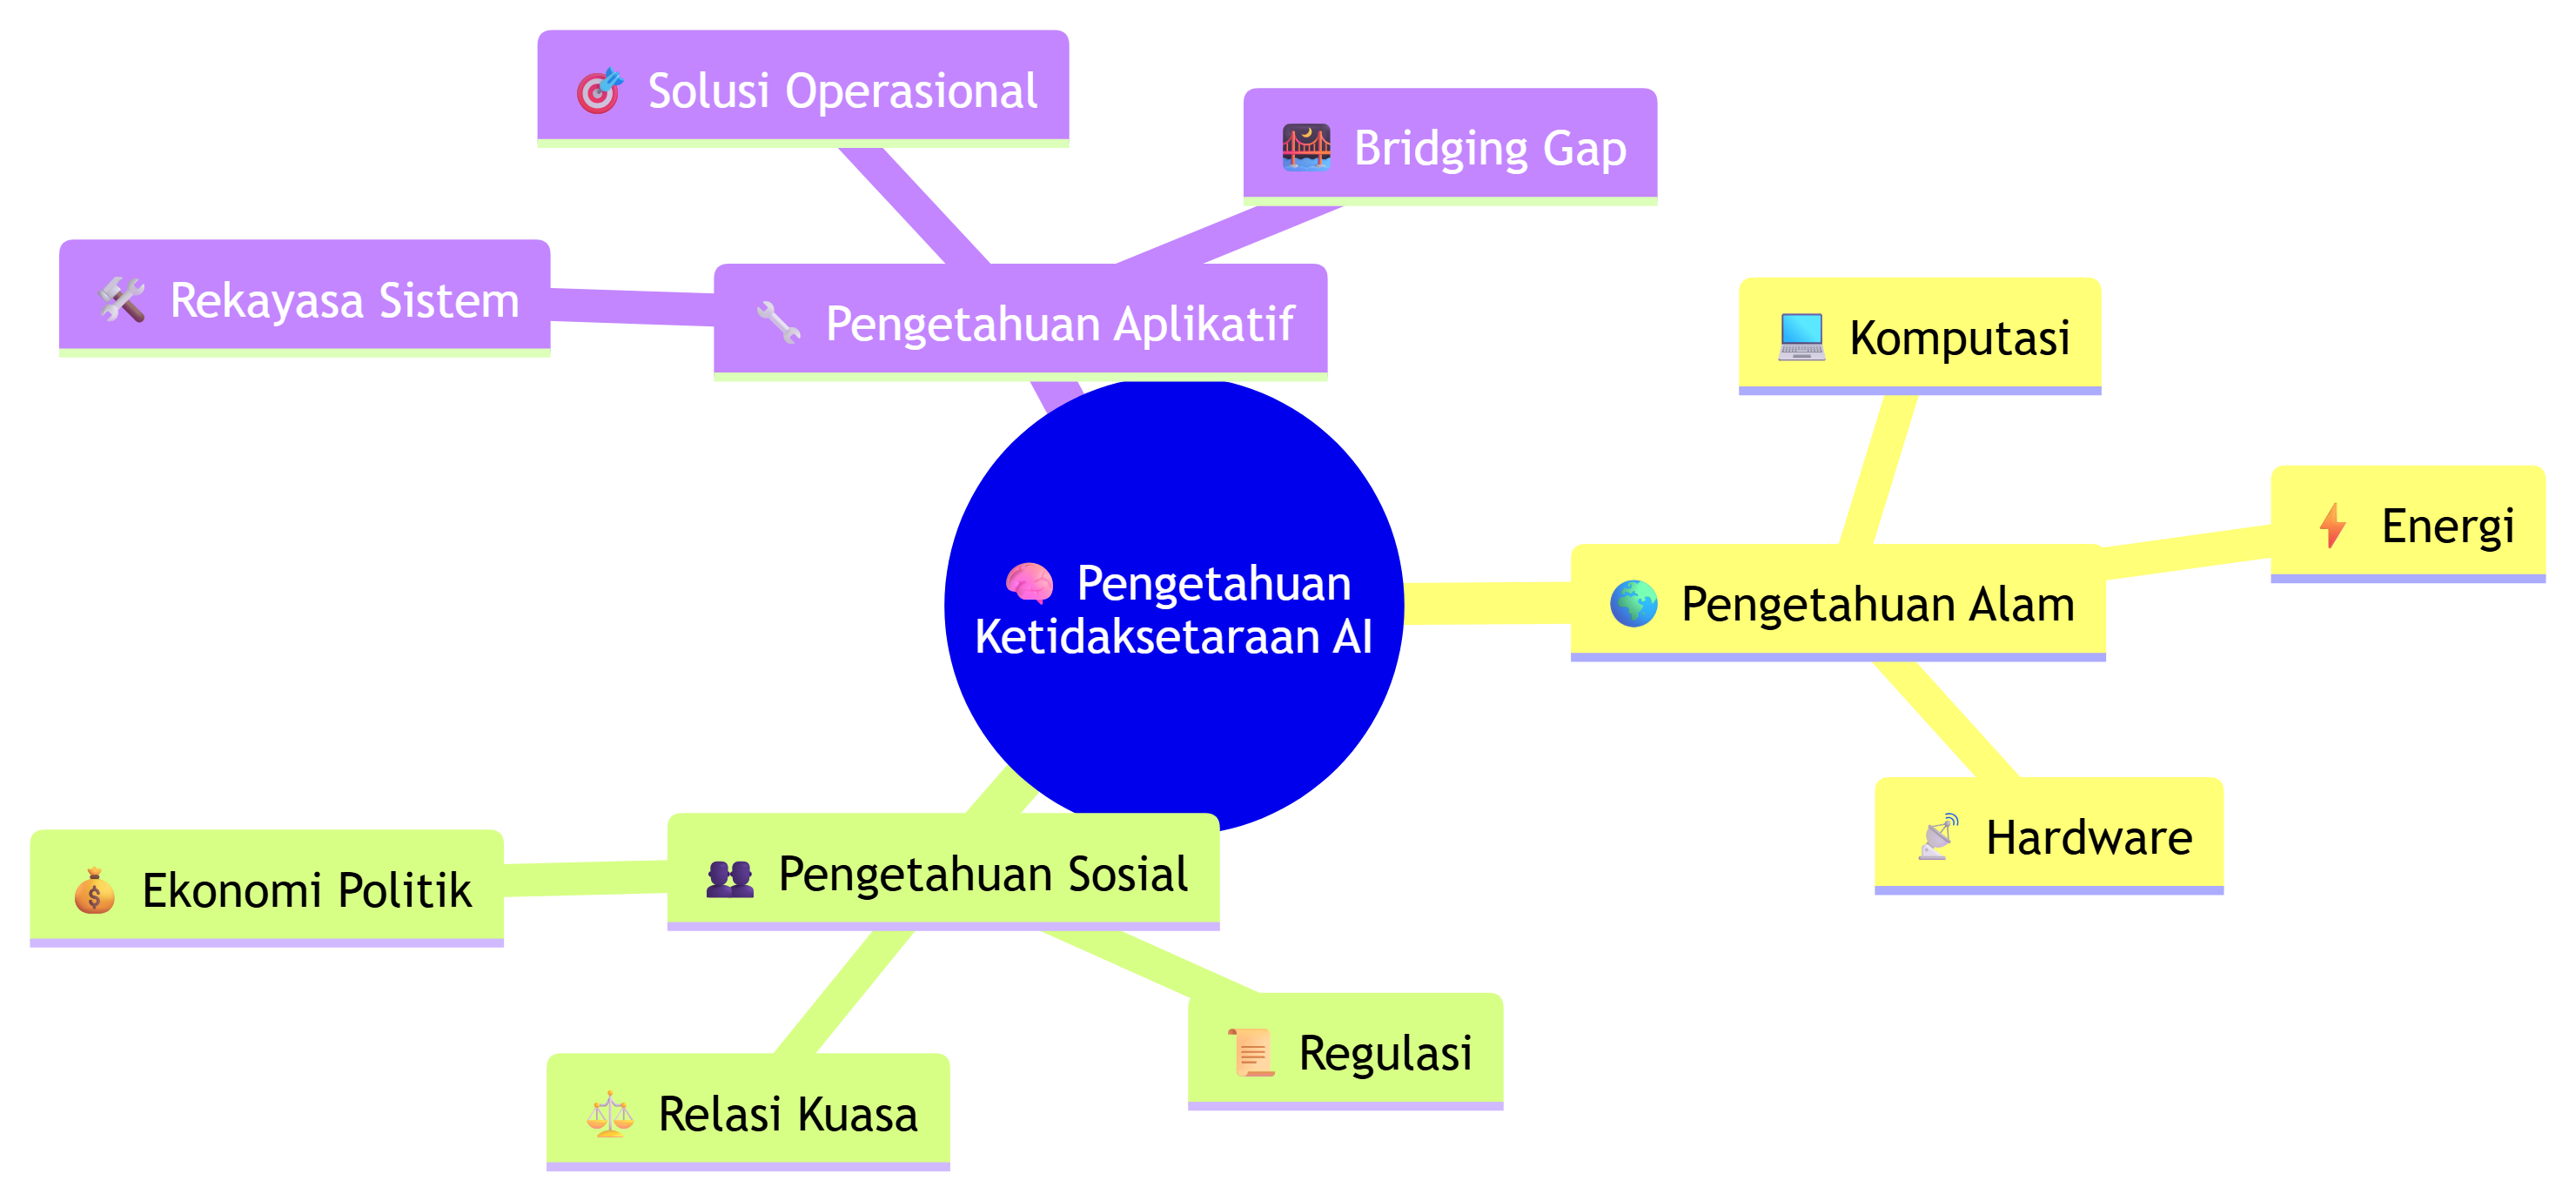
\includegraphics[width=8.94in,height=4.15in]{My_Knowledge/index_files/figure-latex/mermaid-figure-1.png}

\subsection{Hakikat Pengetahuan}\label{hakikat-pengetahuan}

Dalam konteks ketidaksetaraan global di era Artificial Intelligence
(AI), \textbf{pengetahuan berfungsi sebagai deskripsi terstruktur atas
realitas} yang mencakup distribusi sumber daya, akses teknologi, serta
kapasitas komputasi yang tidak merata.

Realitas utama yang dideskripsikan oleh pengetahuan ini meliputi: -
distribusi sumber daya ekonomi, - akses terhadap teknologi dan
infrastruktur digital, - kapasitas komputasi (compute), - serta
kesenjangan pemahaman (knowledge gap).

Isu ini tidak dapat dipahami melalui satu jenis pengetahuan saja,
melainkan merupakan \textbf{kombinasi pengetahuan alam, sosial, dan
aplikatif}, yang saling berinteraksi dalam sistem global.

\begin{center}\rule{0.5\linewidth}{0.5pt}\end{center}

\subsection{Jenis Pengetahuan dalam Ketidaksetaraan
AI}\label{jenis-pengetahuan-dalam-ketidaksetaraan-ai}

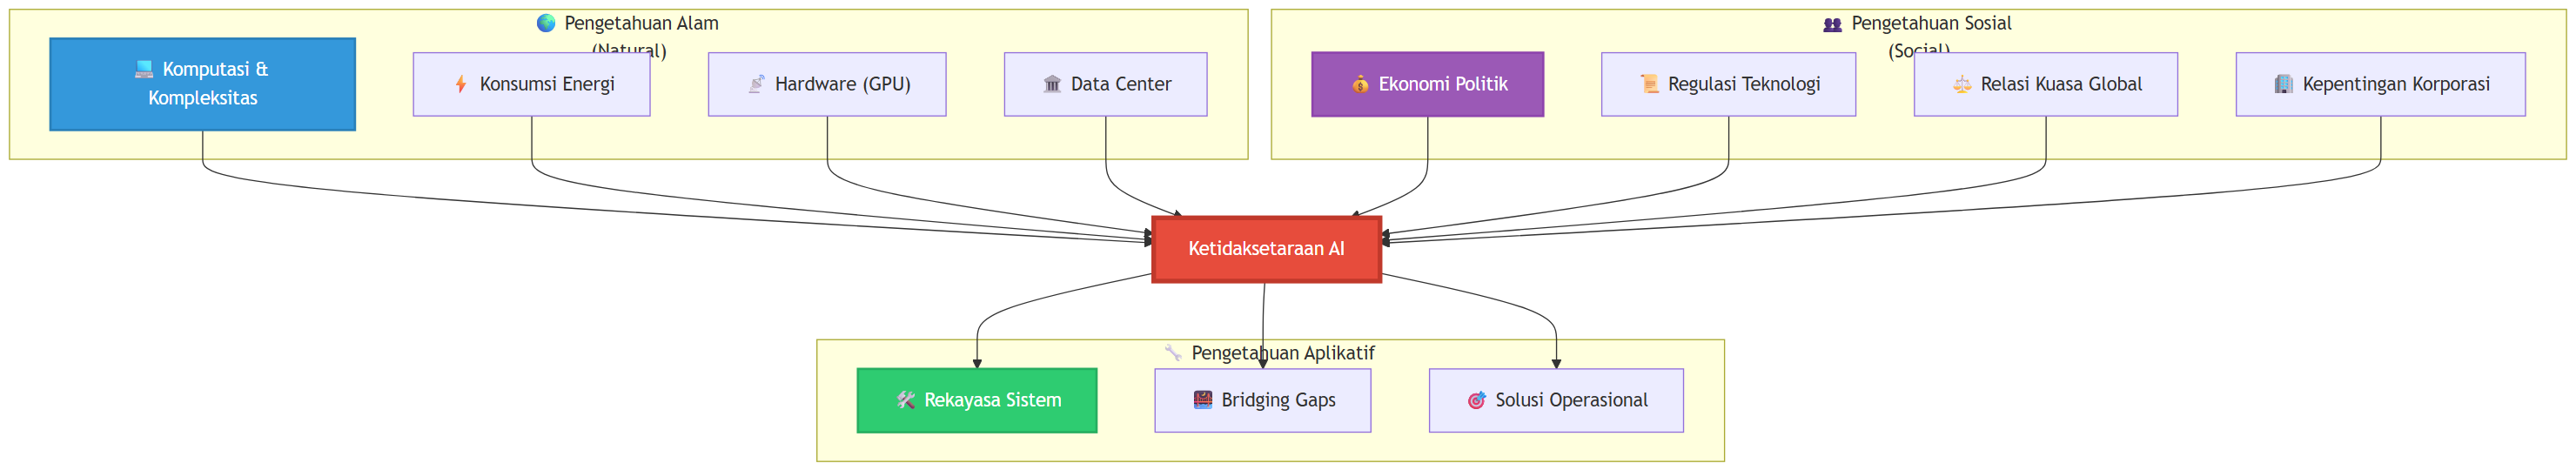
\includegraphics[width=22.91in,height=4.19in]{My_Knowledge/index_files/figure-latex/mermaid-figure-5.png}

\subsubsection{Pengetahuan Alam}\label{pengetahuan-alam}

Pengetahuan alam berperan pada lapisan fisik dan teknis dari AI, antara
lain: - komputasi dan kompleksitas pemrosesan, - konsumsi energi, -
hardware (GPU, accelerator), - jaringan dan bandwidth, - data center
sebagai infrastruktur fisik utama.

Faktor-faktor ini menentukan \textbf{siapa yang mampu membangun,
menjalankan, dan menskalakan AI}, sehingga secara langsung memengaruhi
ketidaksetaraan.

\begin{center}\rule{0.5\linewidth}{0.5pt}\end{center}

\subsubsection{Pengetahuan Sosial}\label{pengetahuan-sosial}

Pengetahuan sosial menjelaskan \textbf{mengapa} ketimpangan tersebut
terjadi dan dipertahankan, terutama melalui: - ekonomi politik, -
regulasi teknologi, - relasi kuasa antara negara maju dan berkembang, -
kepentingan korporasi besar.

Pada lapisan ini, AI tidak lagi netral, melainkan menjadi bagian dari
struktur kekuasaan global.

\begin{center}\rule{0.5\linewidth}{0.5pt}\end{center}

\subsubsection{Pengetahuan Aplikatif}\label{pengetahuan-aplikatif}

Pengetahuan aplikatif berada pada titik temu antara manusia sosial dan
sistem teknologis.\\
Dalam konteks ini, \textbf{rekayasa sistem dan teknologi informasi}
berperan sebagai alat untuk: - mengubah kapasitas kerja manusia menjadi
kekuatan sistemik, - memindahkan ``beban'' ketidaksetaraan dari titik
ketidakberdayaan menuju solusi yang dapat dioperasionalkan, - merancang
sistem yang menjembatani keterbatasan akses dan pengetahuan.

\begin{center}\rule{0.5\linewidth}{0.5pt}\end{center}

\subsection{Klasifikasi Pengetahuan Berdasarkan Taksonomi
Bloom}\label{klasifikasi-pengetahuan-berdasarkan-taksonomi-bloom}

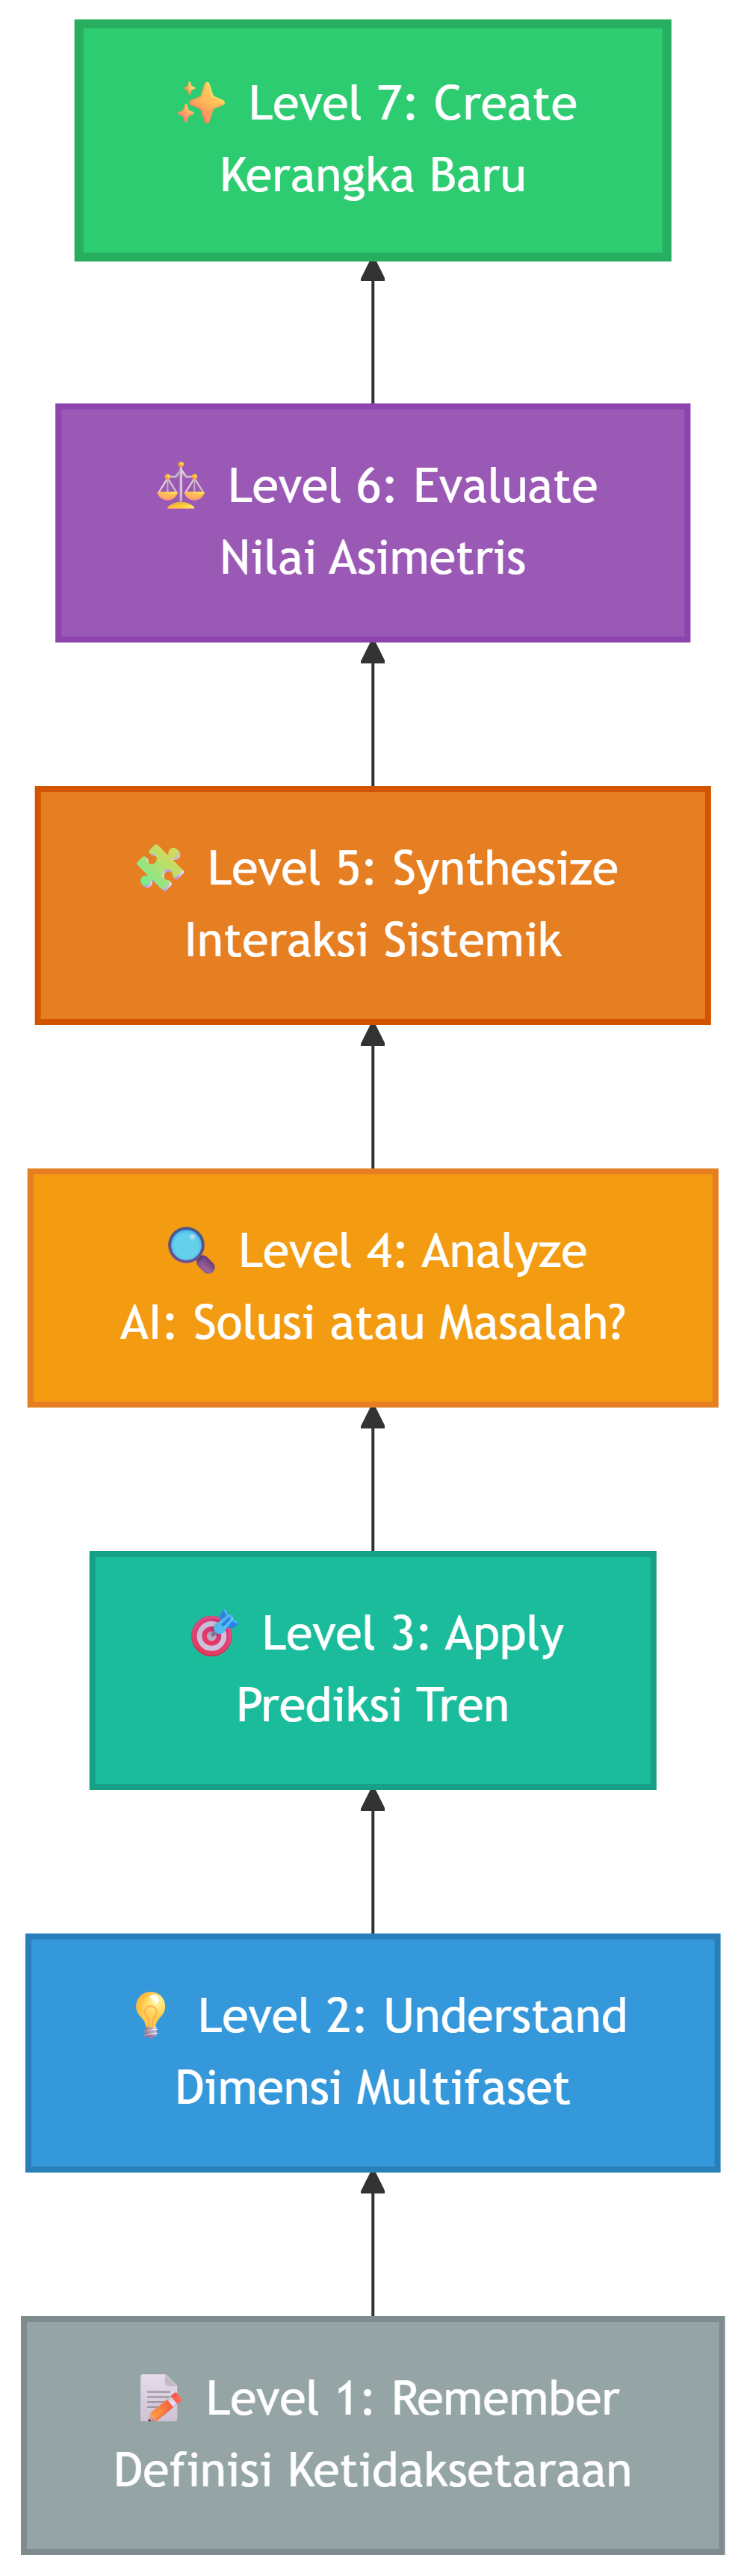
\includegraphics[width=2.6in,height=8.98in]{My_Knowledge/index_files/figure-latex/mermaid-figure-4.png}

\begin{figure}[H]

{\centering \pandocbounded{\includegraphics[keepaspectratio]{index_files/mediabag/photo-1503676260728-.jpg}}

}

\caption{Bloom's Taxonomy}

\end{figure}%

\subsubsection{Level 1 --- Remember}\label{level-1-remember}

Pengetahuan dasar mencakup: - definisi ketidaksetaraan global sebagai
pelebaran jarak akses dan distribusi manfaat, - pemahaman bahwa tidak
semua permasalahan dapat dan seharusnya diselesaikan dengan AI.

\begin{center}\rule{0.5\linewidth}{0.5pt}\end{center}

\subsubsection{Level 2 --- Understand}\label{level-2-understand}

Ketidaksetaraan global di era AI dapat diklasifikasikan ke dalam
beberapa dimensi: - ekonomi, - teknologi, - budaya (misalnya hedonisme
dan konsumsi teknologi), - pengetahuan, - data.

Klasifikasi ini membantu memahami bahwa ketimpangan bersifat
multidimensional.

\begin{center}\rule{0.5\linewidth}{0.5pt}\end{center}

\subsubsection{Level 3 --- Apply}\label{level-3-apply}

Dengan menerapkan pemahaman tersebut, dapat diprediksi bahwa
\textbf{jika tren AI saat ini berlanjut tanpa koreksi}, maka: -
ketergantungan manusia terhadap AI akan meningkat, - ketimpangan akan
melebar, - dan fokus penggunaan AI akan bergeser dari riset menuju
tujuan rekreasional dan komersial.

\begin{center}\rule{0.5\linewidth}{0.5pt}\end{center}

\subsubsection{Level 4 --- Analyze}\label{level-4-analyze}

AI dapat sekaligus mengurangi dan menciptakan ketidaksetaraan karena: -
tingginya kebutuhan komputasi dan energi, - sentralisasi data dan model,
- dominasi negara dan perusahaan besar.

Fenomena ini menyerupai \textbf{``The Second Space Race''}, di mana
inovasi objektif yang bermanfaat bagi manusia justru berubah menjadi
ajang pamer kekuatan dan pemborosan sumber daya.

\begin{center}\rule{0.5\linewidth}{0.5pt}\end{center}

\subsubsection{Level 5 --- Synthesize}\label{level-5-synthesize}

Pada tahap sintesis, elemen-elemen tersebut dapat disusun menjadi
pemahaman bahwa:

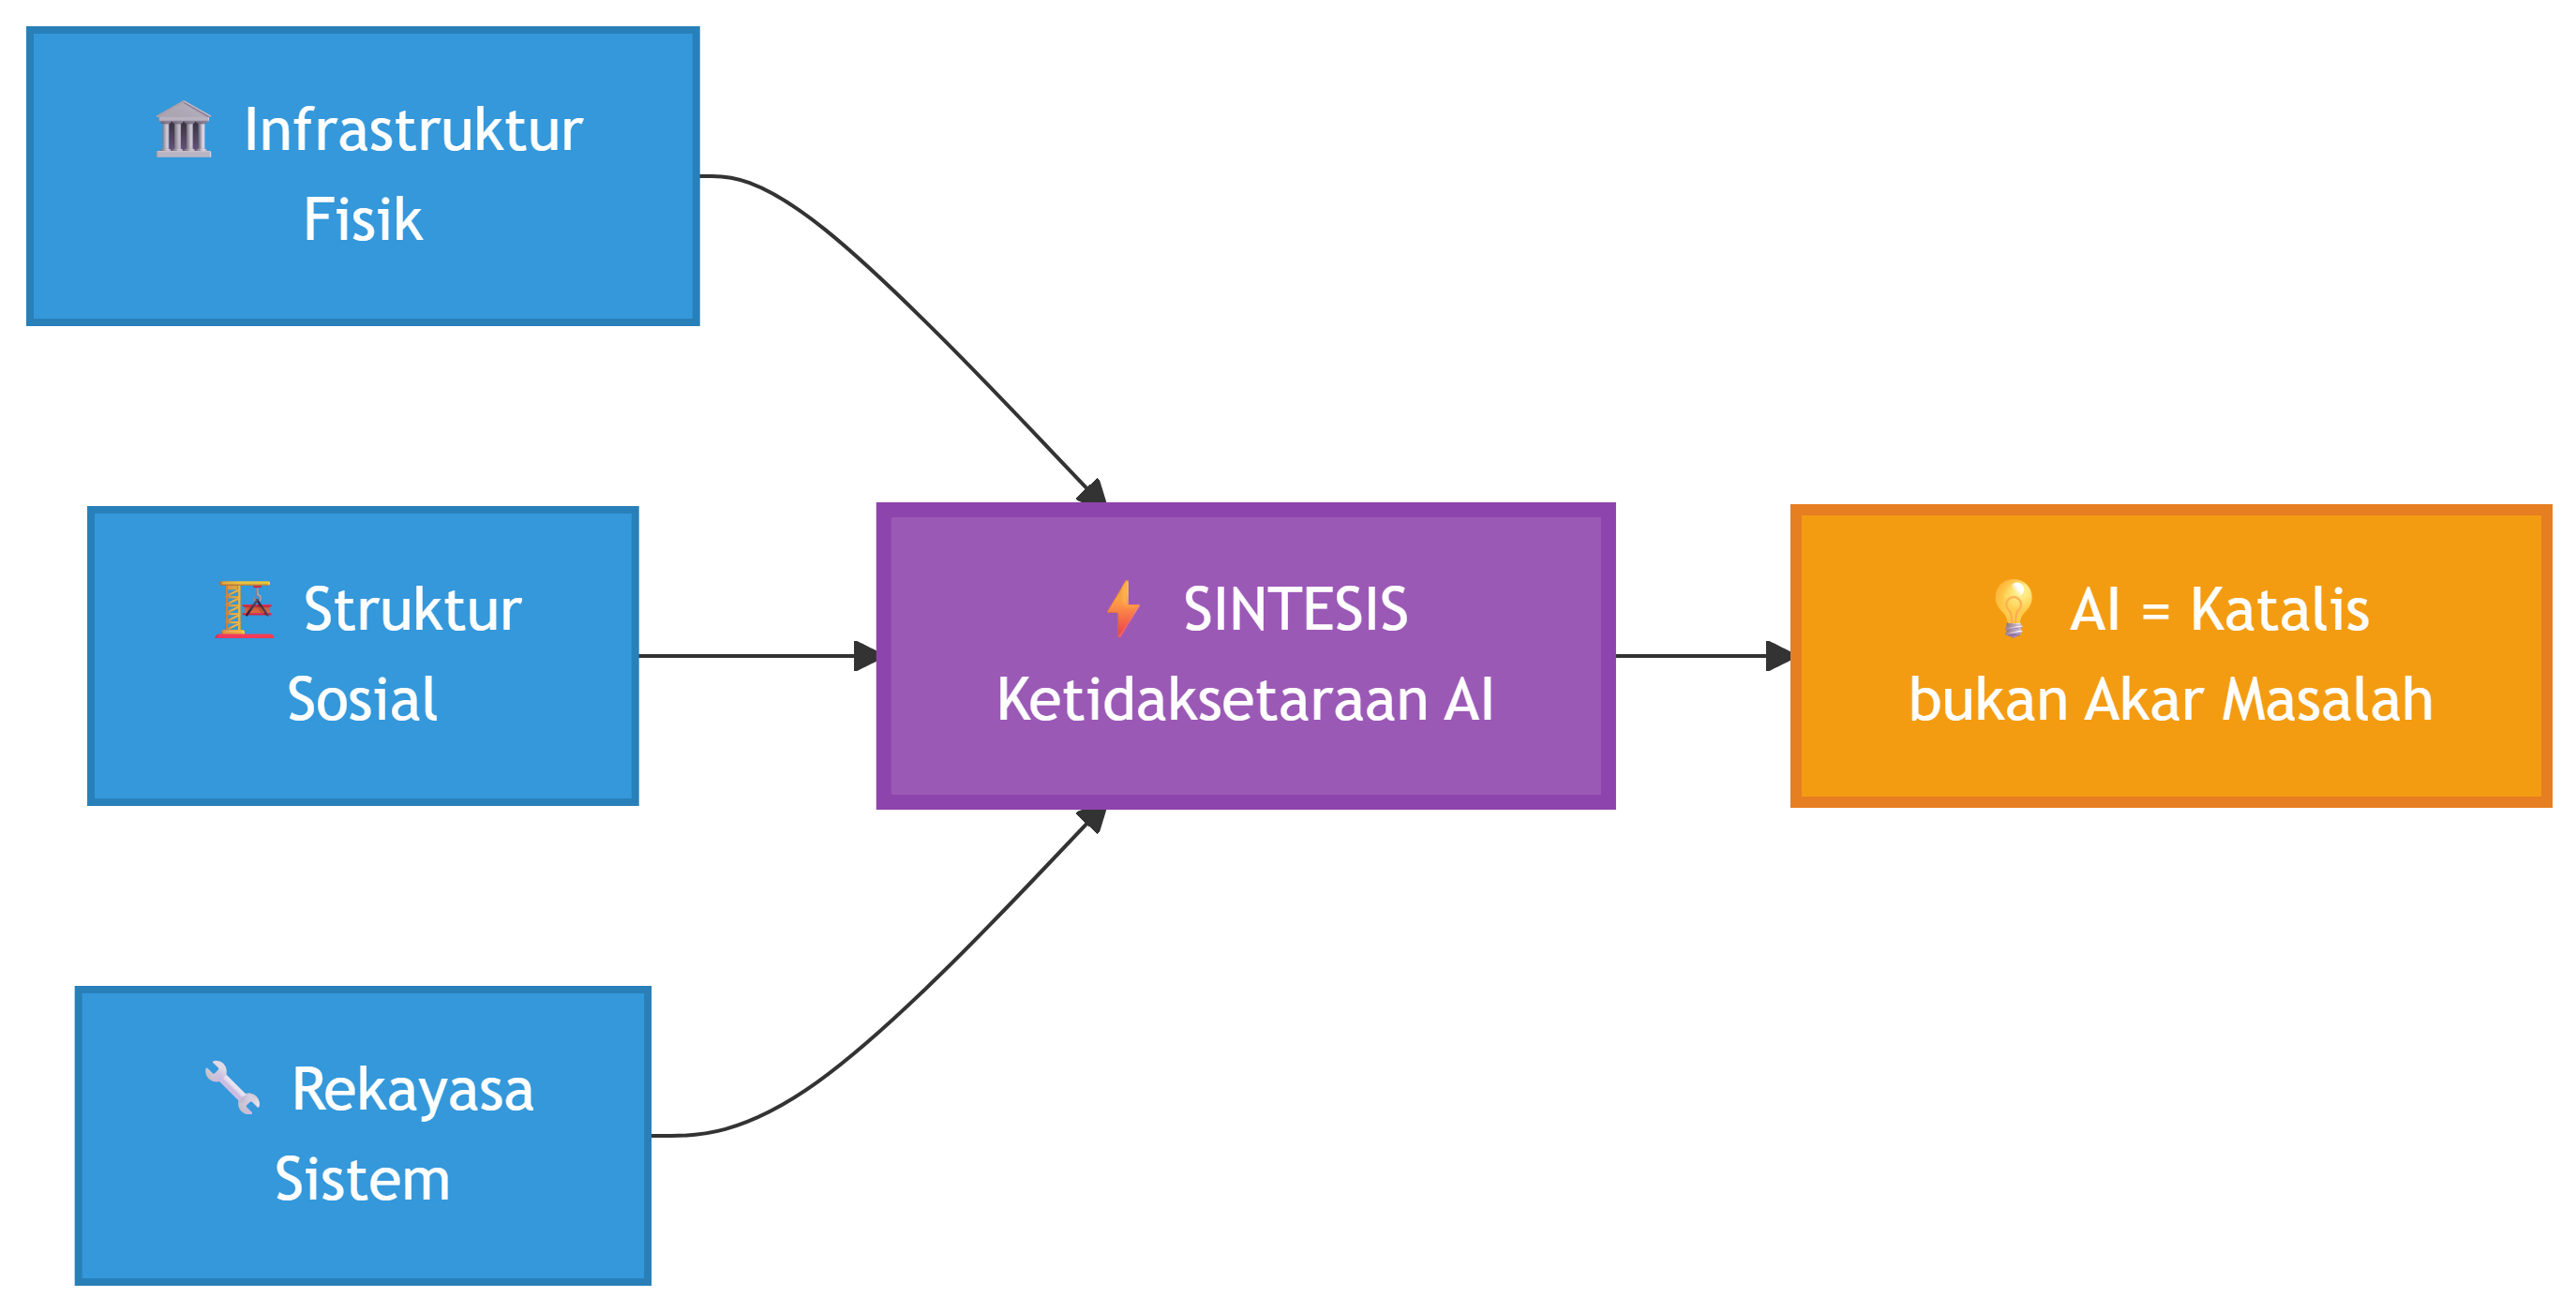
\includegraphics[width=7.16in,height=3.65in]{My_Knowledge/index_files/figure-latex/mermaid-figure-3.png}

\begin{quote}
Ketidaksetaraan global di era AI bukan semata akibat teknologi,
melainkan hasil interaksi antara infrastruktur fisik, struktur sosial,
dan arah rekayasa sistem.
\end{quote}

AI adalah katalis---bukan akar masalah---yang mempercepat dinamika
ketimpangan yang sudah ada.

\begin{center}\rule{0.5\linewidth}{0.5pt}\end{center}

\subsubsection{Level 6 --- Evaluate}\label{level-6-evaluate}

Dari sudut pandang evaluatif: - bagi perusahaan besar, AI bernilai
positif karena efisiensi dan pemotongan biaya, - bagi masyarakat luas,
AI cenderung bernilai negatif karena berkurangnya lapangan kerja dan
meningkatnya ketergantungan sistemik.

Nilai AI bersifat \textbf{asimetris}, tergantung posisi aktor dalam
sistem.

\begin{center}\rule{0.5\linewidth}{0.5pt}\end{center}

\subsubsection{Level 7 --- Create}\label{level-7-create}

Sebagai entitas baru, dapat dirancang \textbf{kerangka sistem AI
berbasis aksesibilitas dan literasi pengetahuan}, yang: -
memprioritaskan distribusi pengetahuan dibanding akumulasi model, -
menempatkan AI sebagai alat pendukung manusia, bukan pengganti.

\begin{center}\rule{0.5\linewidth}{0.5pt}\end{center}

\subsection{Knowledge Maps}\label{knowledge-maps}

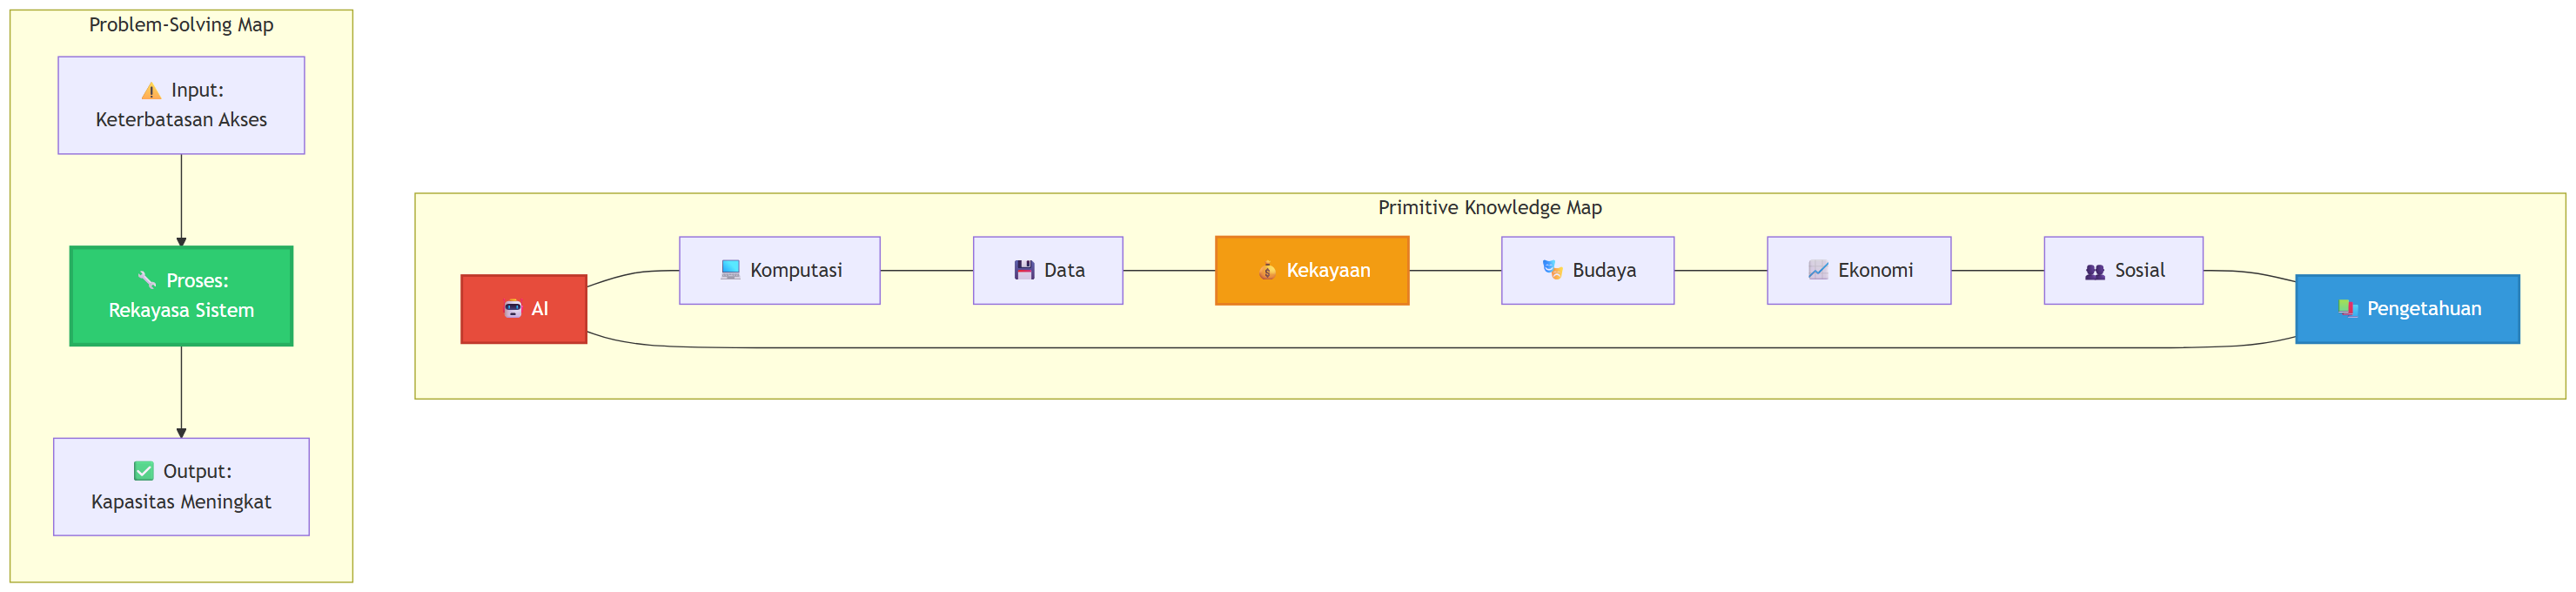
\includegraphics[width=21.53in,height=4.95in]{My_Knowledge/index_files/figure-latex/mermaid-figure-2.png}

\subsubsection{Primitive Knowledge Map}\label{primitive-knowledge-map}

Node utama dalam peta pengetahuan primitif meliputi: - AI - Komputasi -
Data - Kekayaan - Budaya - Ekonomi - Sosial - Pengetahuan (Knowledge)

Peta ini berfungsi sebagai \textbf{badan pengetahuan deklaratif} tentang
``apa'' yang membentuk ketidaksetaraan global di era AI.

\begin{center}\rule{0.5\linewidth}{0.5pt}\end{center}

\subsubsection{Problem-Solving Knowledge
Map}\label{problem-solving-knowledge-map}

Masalah utama yang dapat ditangani secara rekayasa adalah:

\begin{quote}
\textbf{Keterbatasan akses dan pemahaman terhadap AI.}
\end{quote}

Secara garis besar: - \textbf{Input:} keterbatasan akses teknologi dan
literasi, - \textbf{Proses:} rekayasa sistem pembelajaran dan distribusi
pengetahuan, - \textbf{Output:} peningkatan kapasitas manusia tanpa
ketergantungan berlebih pada AI.

\begin{center}\rule{0.5\linewidth}{0.5pt}\end{center}

\subsection{Produk Pengetahuan}\label{produk-pengetahuan}

Produk pengetahuan yang paling relevan untuk topik ini meliputi: - Peta
Pengetahuan Primitif, - Peta Pemecahan Masalah, - dan jurnal pembelajar
reflektif.

Produk-produk ini merepresentasikan pemahaman yang tidak berhenti pada
hafalan, tetapi mampu memandu tindakan rekayasa.

\begin{center}\rule{0.5\linewidth}{0.5pt}\end{center}

\subsection{Meta-Pengetahuan
(Refleksi)}\label{meta-pengetahuan-refleksi}

Pengetahuan tentang struktur ketidaksetaraan dan peran AI telah relatif
kuat pada level analisis dan evaluasi.\\
Namun, pengetahuan aplikatif masih perlu dikembangkan lebih lanjut agar
mampu menghasilkan solusi sistemik yang nyata dan berkelanjutan.

\begin{center}\rule{0.5\linewidth}{0.5pt}\end{center}

\subsection{Penutup}\label{penutup-1}

Pengetahuan tentang ketidaksetaraan global di era Artificial
Intelligence berfungsi sebagai \textbf{cetak biru (blueprint)} bagi
rekayasa sistem.\\
Dengan pengetahuan yang terstruktur, manusia dapat mengarahkan kekuatan
teknologi bukan untuk sekadar menunjukkan kecanggihan, tetapi untuk
memindahkan beban sosial menuju arah yang lebih adil dan bermakna.

\bookmarksetup{startatroot}

\chapter{UAS-4 My Innovations}\label{uas-4-my-innovations}

\begin{figure}[H]

{\centering \pandocbounded{\includegraphics[keepaspectratio]{index_files/mediabag/giphy123.gif}}

}

\caption{Innovation}

\end{figure}%

\section{Value Innovation in the Era of Artificial
Intelligence}\label{value-innovation-in-the-era-of-artificial-intelligence}

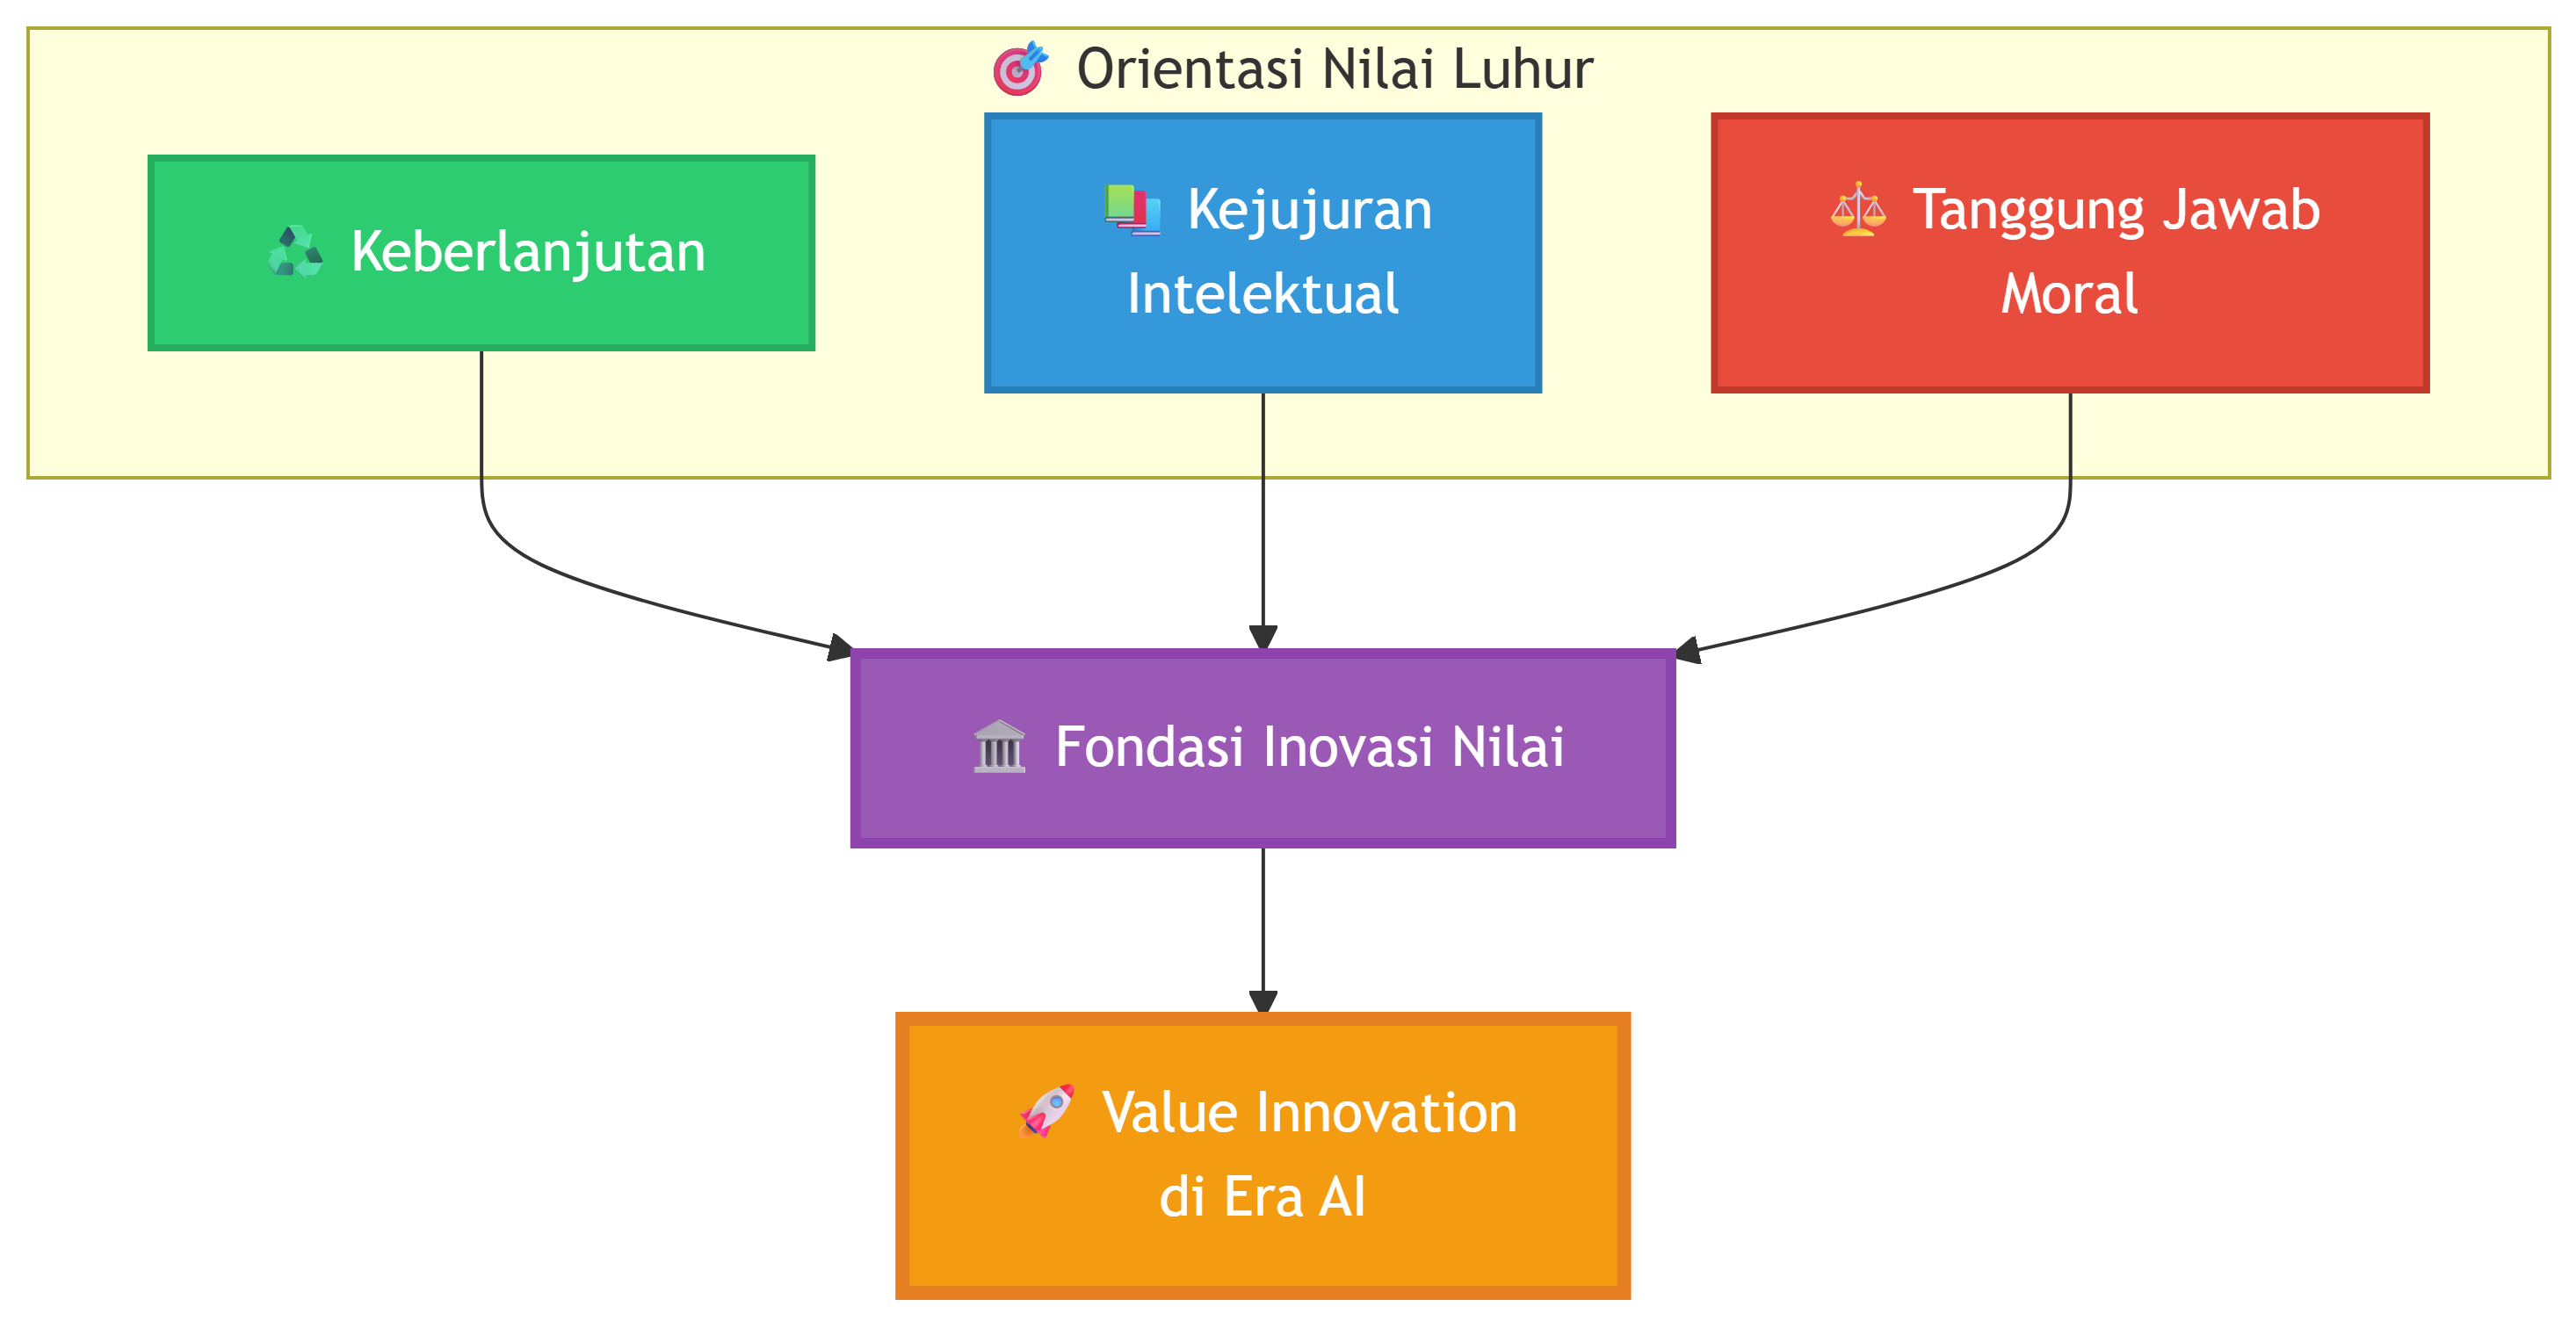
\includegraphics[width=7.64in,height=3.92in]{My_Innovations/index_files/figure-latex/mermaid-figure-1.png}

\subsection{Orientasi Nilai Luhur}\label{orientasi-nilai-luhur}

Inovasi nilai yang saya tawarkan berangkat dari tiga nilai utama:

\begin{enumerate}
\def\labelenumi{\arabic{enumi}.}
\tightlist
\item
  \textbf{Keberlanjutan}\\
\item
  \textbf{Kejujuran Intelektual}\\
\item
  \textbf{Tanggung Jawab Moral}
\end{enumerate}

Nilai-nilai ini menjadi fondasi dalam merancang sistem dan teknologi
informasi di era Artificial Intelligence (AI), terutama ketika teknologi
tersebut memiliki dampak langsung terhadap ketidaksetaraan global.

Saya meyakini bahwa inovasi tanpa orientasi nilai hanya akan
menghasilkan efisiensi jangka pendek, tetapi kerusakan jangka panjang
pada manusia dan masyarakat.

\begin{center}\rule{0.5\linewidth}{0.5pt}\end{center}

\subsection{Masalah Nilai yang Terjadi Saat
Ini}\label{masalah-nilai-yang-terjadi-saat-ini}

Dalam praktik pengembangan AI saat ini, nilai yang paling sering hilang
adalah:

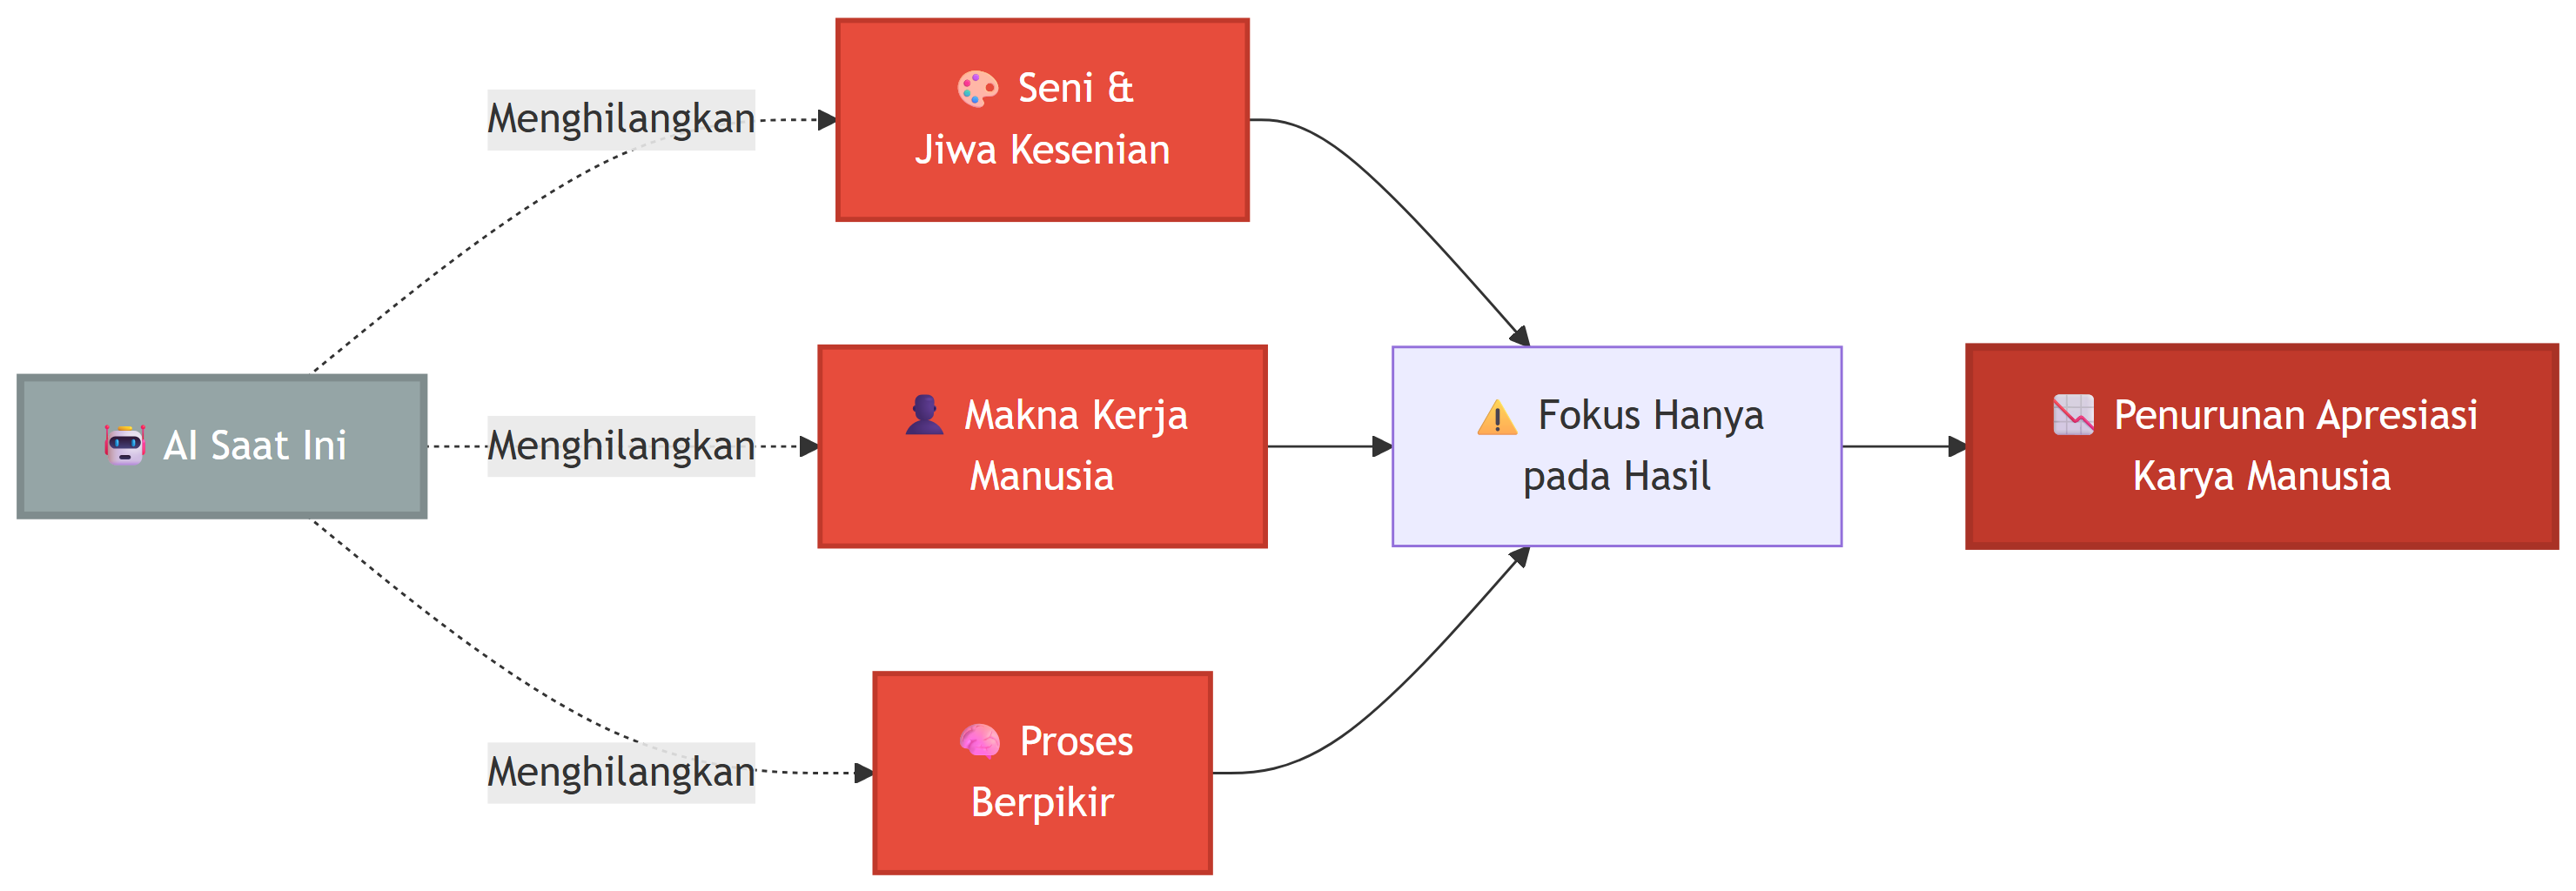
\includegraphics[width=10.51in,height=3.65in]{My_Innovations/index_files/figure-latex/mermaid-figure-5.png}

\begin{itemize}
\tightlist
\item
  \textbf{seni dan jiwa kesenian},\\
\item
  \textbf{makna kerja manusia},\\
\item
  dan \textbf{proses berpikir itu sendiri}.
\end{itemize}

AI sering diposisikan sebagai pengganti, bukan pendukung. Hal ini
mengikis nilai proses, menjadikan hasil sebagai satu-satunya ukuran
keberhasilan, dan pada akhirnya menurunkan apresiasi terhadap karya
manusia.

\begin{center}\rule{0.5\linewidth}{0.5pt}\end{center}

\subsection{Ketidaksetaraan sebagai Kegagalan Pendidikan
Nilai}\label{ketidaksetaraan-sebagai-kegagalan-pendidikan-nilai}

\begin{figure}[H]

{\centering \pandocbounded{\includegraphics[keepaspectratio]{index_files/mediabag/photo-1503676260728-.jpg}}

}

\caption{Education}

\end{figure}%

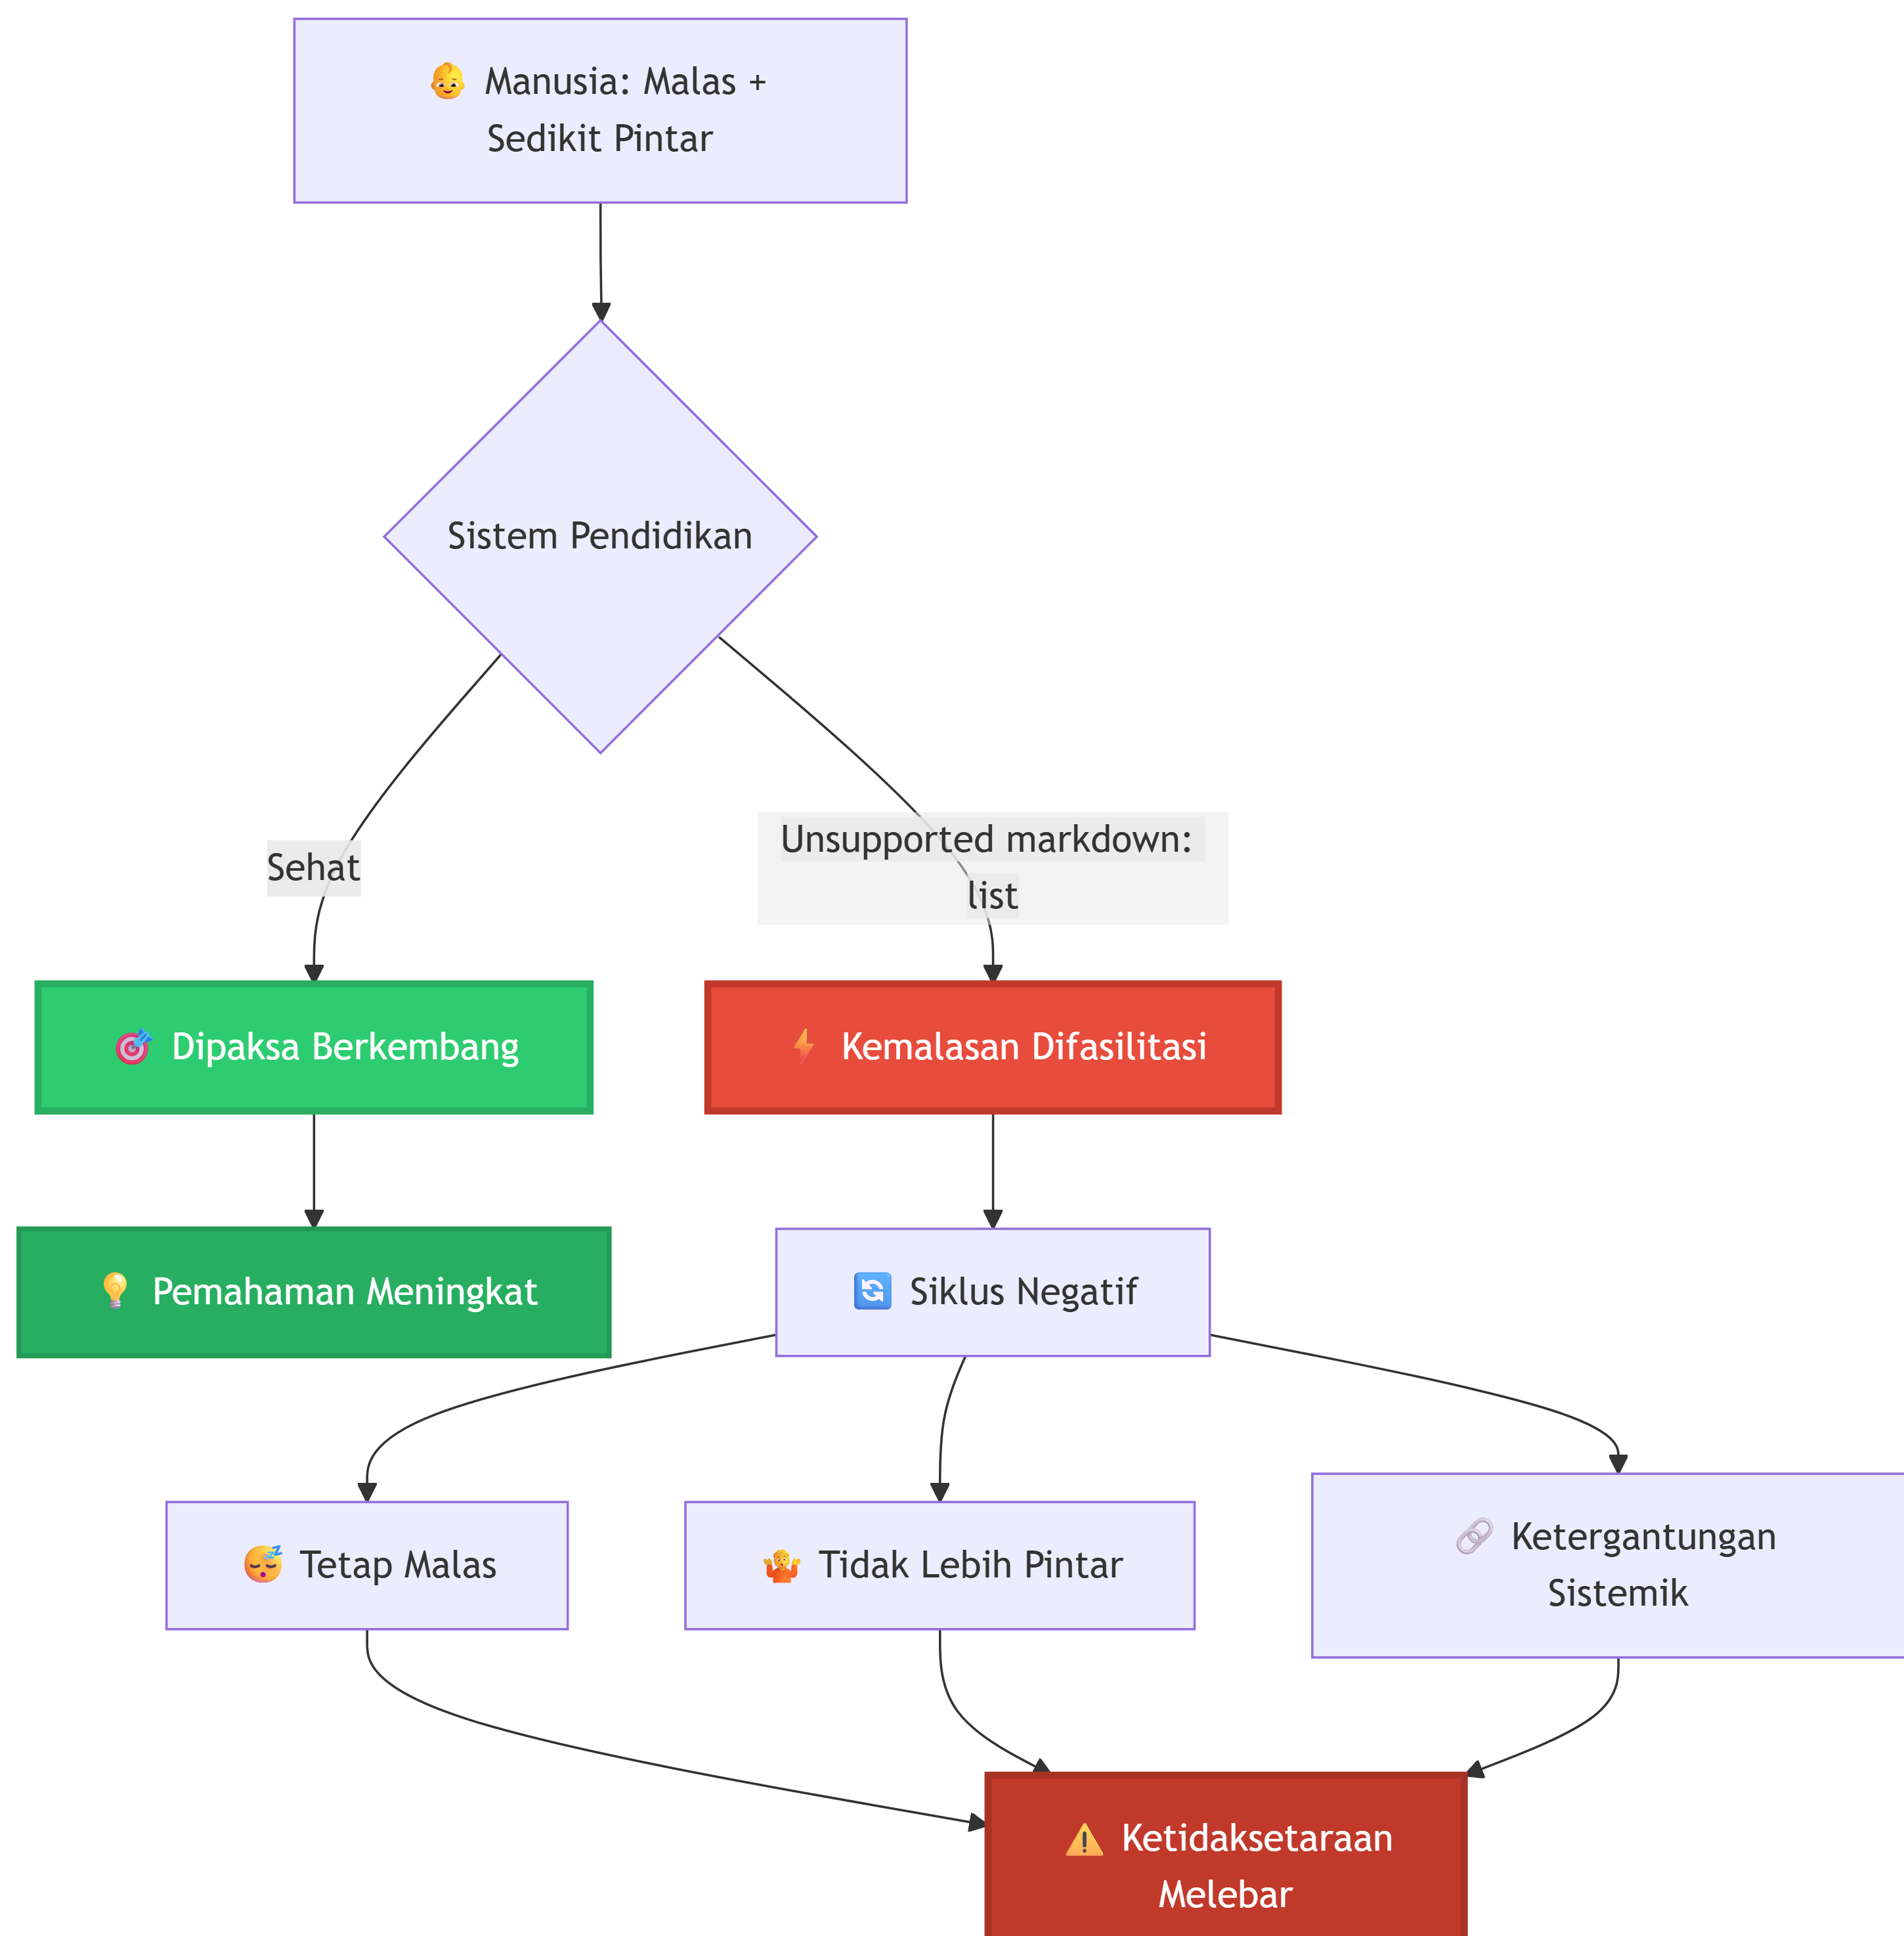
\includegraphics[width=8.6in,height=8.75in]{My_Innovations/index_files/figure-latex/mermaid-figure-4.png}

Saya melihat ketidaksetaraan global di era AI terutama sebagai
\textbf{kegagalan pendidikan}, bukan semata kegagalan teknologi.

Manusia pada dasarnya cenderung malas, namun sedikit pintar. Dalam
sistem pendidikan yang sehat, kemalasan tersebut ``dipaksa'' untuk
berkembang menjadi pemahaman. Dengan hadirnya AI, kemalasan itu justru
difasilitasi---tanpa diimbangi peningkatan kapasitas berpikir.

Akibatnya, manusia: - tetap malas, - tidak menjadi lebih pintar, - dan
semakin bergantung pada sistem.

\begin{center}\rule{0.5\linewidth}{0.5pt}\end{center}

\subsection{Distribusi Nilai yang Tidak
Adil}\label{distribusi-nilai-yang-tidak-adil}

Dalam ekosistem AI saat ini, saya berpendapat bahwa: - \textbf{tidak ada
pihak yang benar-benar menciptakan nilai baru}, dan - \textbf{manusia
itu sendiri adalah pihak yang paling sedikit menerima nilai}.

Nilai tereduksi menjadi penghematan biaya, sementara dampak sosial,
budaya, dan manusiawi diabaikan.

\begin{center}\rule{0.5\linewidth}{0.5pt}\end{center}

\subsection{Posisi dalam Knowledge
Marketplace}\label{posisi-dalam-knowledge-marketplace}

Sebagai respons terhadap kebutuhan pembelajaran dan rekayasa, kebutuhan
nilai yang layak ``diiklankan'' dalam Knowledge Marketplace adalah:

\begin{itemize}
\tightlist
\item
  sistem AI yang inklusif,
\item
  peta pengetahuan tentang ketimpangan AI,
\item
  dan kerangka etika berbasis rekayasa.
\end{itemize}

Sebagai mahasiswa, kontribusi nilai yang realistis bukanlah membangun AI
baru, melainkan \textbf{menghasilkan artefak reflektif berbasis sejarah,
bukti nyata, dan analisis sistemik}.

\begin{center}\rule{0.5\linewidth}{0.5pt}\end{center}

\subsection{\texorpdfstring{Bentuk Inovasi Nilai: \emph{AI Usage
Boundary
Model}}{Bentuk Inovasi Nilai: AI Usage Boundary Model}}\label{bentuk-inovasi-nilai-ai-usage-boundary-model}

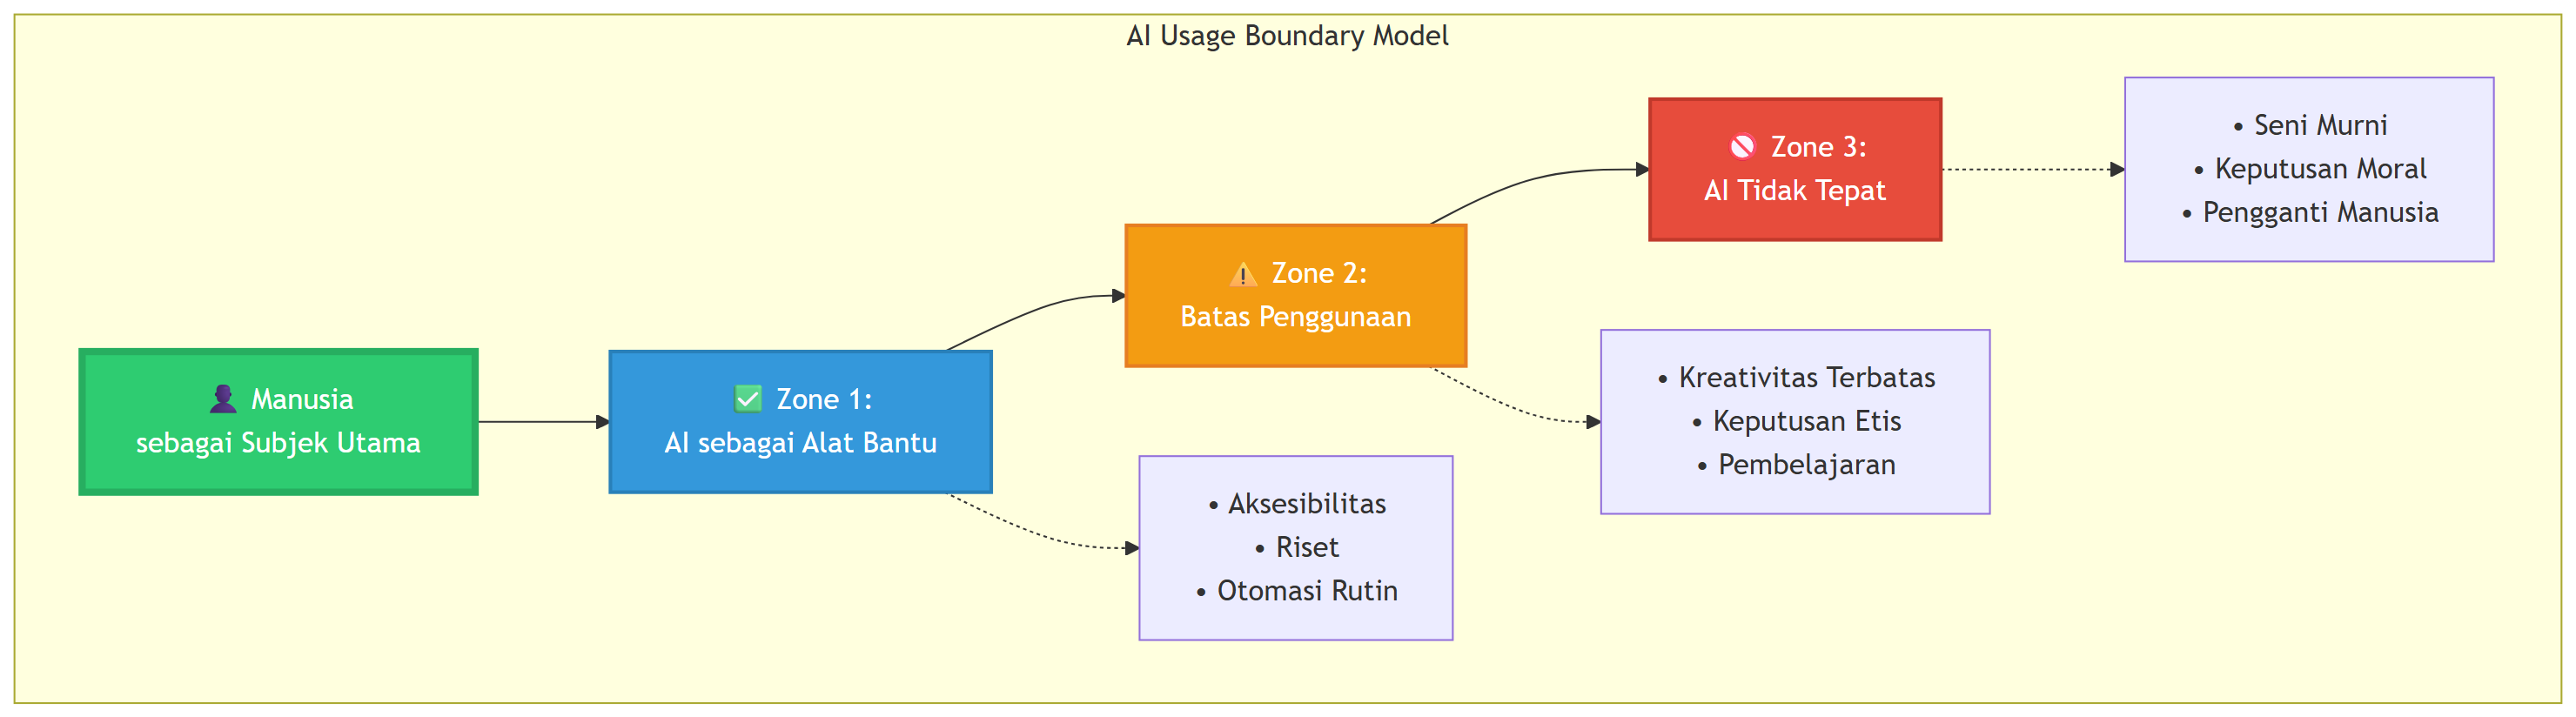
\includegraphics[width=14.88in,height=4.15in]{My_Innovations/index_files/figure-latex/mermaid-figure-3.png}

Bentuk inovasi nilai yang saya ajukan adalah \textbf{AI Usage Boundary
Model}.

Model ini bukan untuk melarang AI, melainkan untuk: - menetapkan
\textbf{batas penggunaan AI},\\
- menempatkan AI sebagai alat bantu, bukan pusat solusi,\\
- dan mengembalikan manusia sebagai subjek utama.

\begin{center}\rule{0.5\linewidth}{0.5pt}\end{center}

\subsection{Nilai Baru yang
Diciptakan}\label{nilai-baru-yang-diciptakan}

Inovasi ini menciptakan nilai-nilai berikut:

\begin{itemize}
\tightlist
\item
  \textbf{rasa kepemilikan terhadap proses berpikir},\\
\item
  \textbf{kesadaran batas AI},\\
\item
  \textbf{literasi ketimpangan global berbasis AI},\\
\item
  \textbf{penguatan peran manusia},\\
\item
  serta \textbf{kesadaran akan ketidakadilan yang dihasilkan oleh sistem
  AI}.
\end{itemize}

Nilai-nilai ini tidak muncul dari fitur teknis, tetapi dari perubahan
cara pandang.

\begin{center}\rule{0.5\linewidth}{0.5pt}\end{center}

\subsection{Value Co-Creation: Semua
Terlibat}\label{value-co-creation-semua-terlibat}

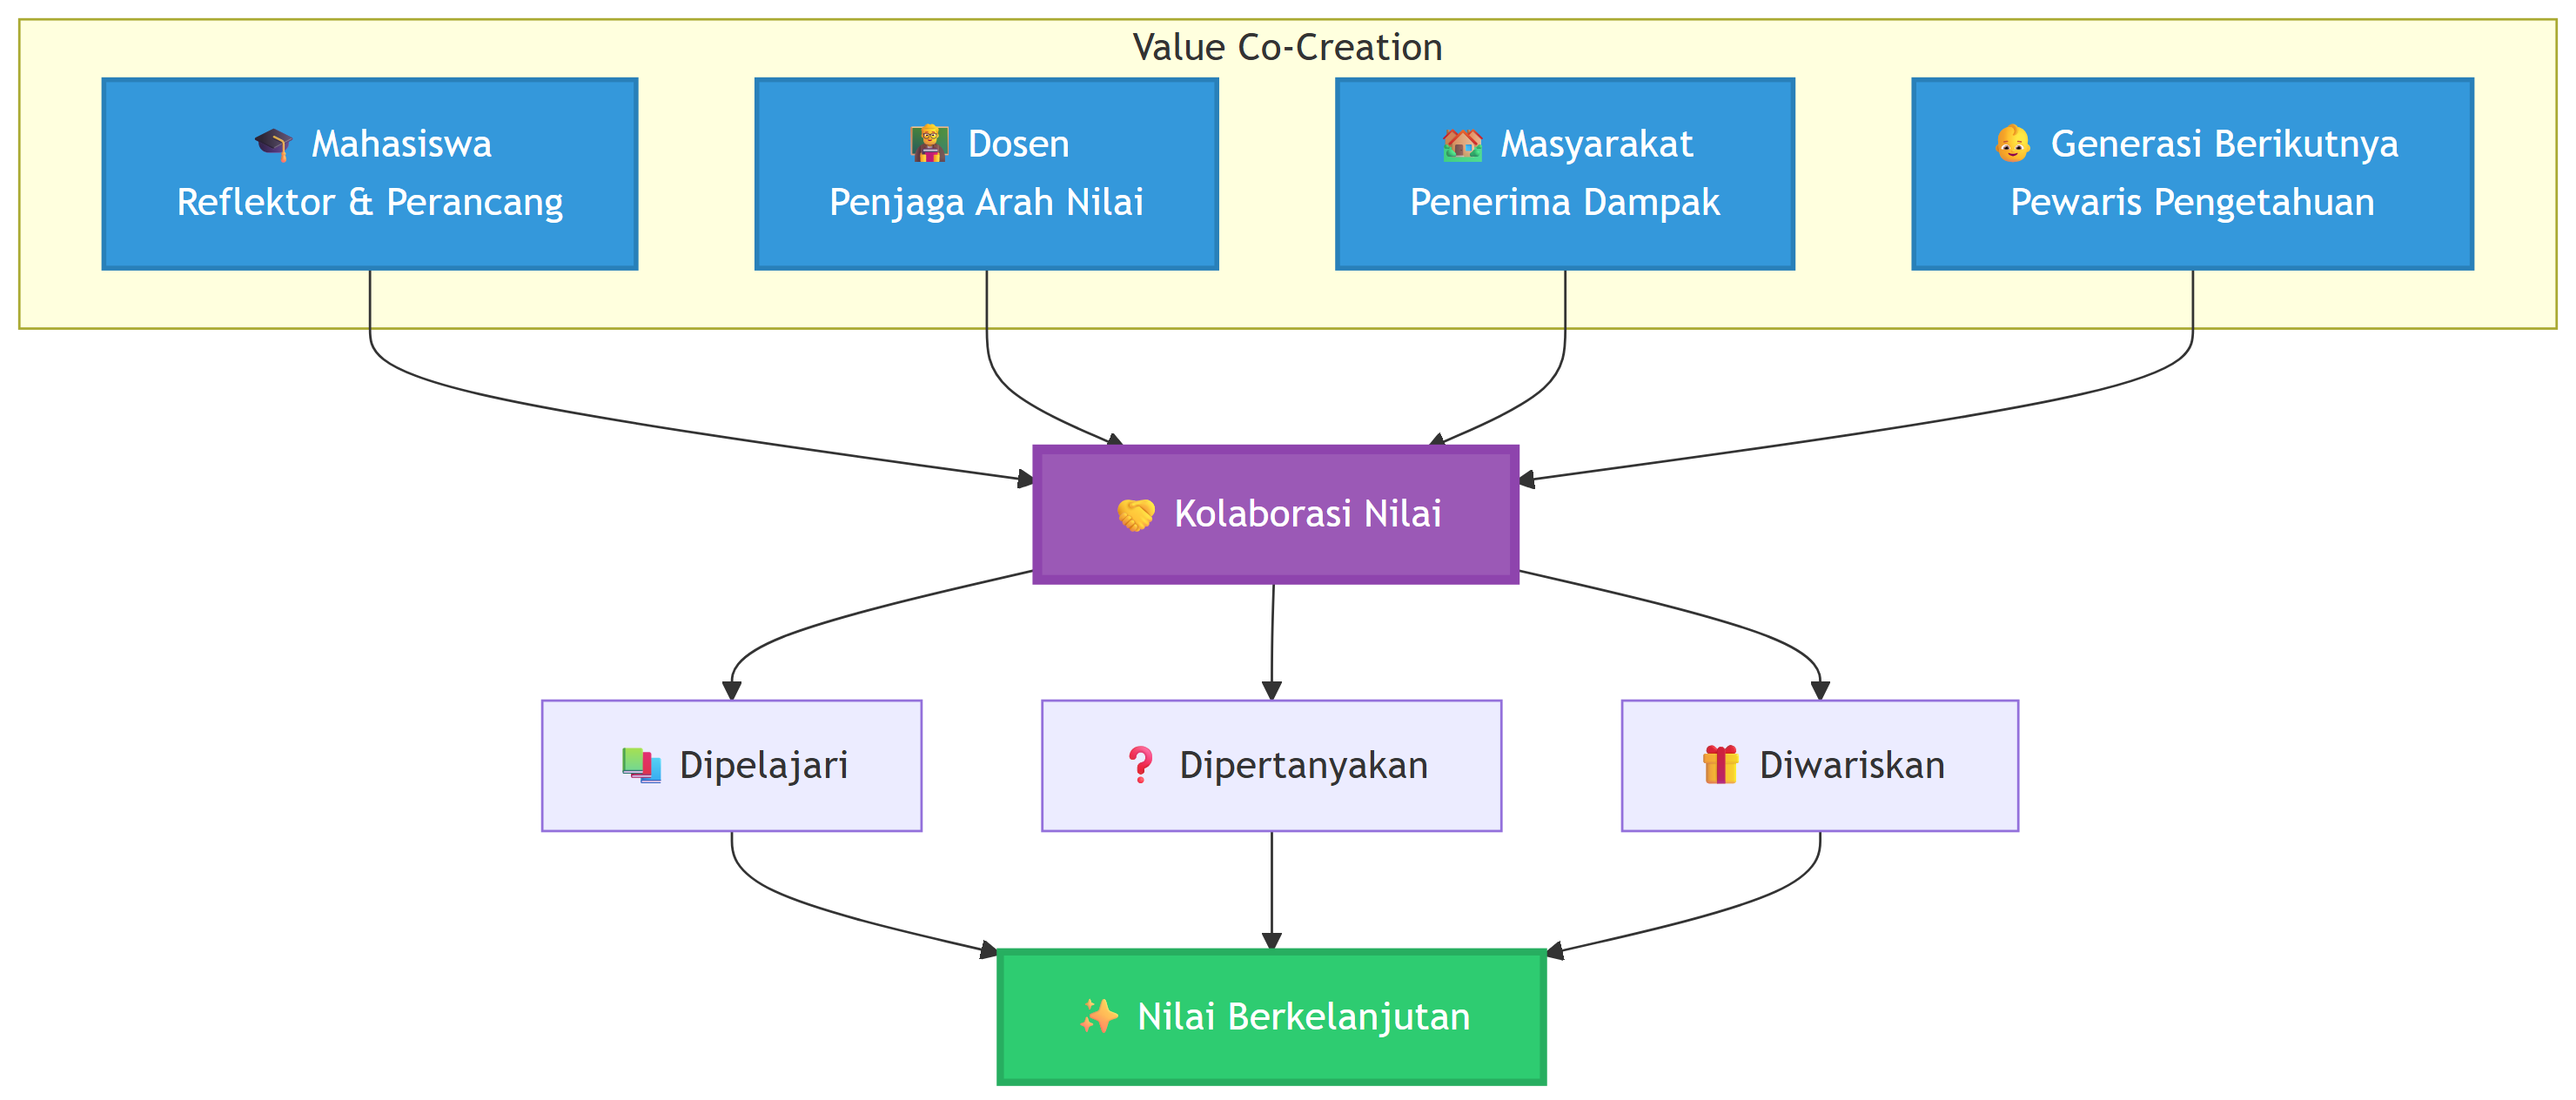
\includegraphics[width=11.11in,height=4.75in]{My_Innovations/index_files/figure-latex/mermaid-figure-2.png}

Penciptaan nilai dalam inovasi ini bersifat kolektif.

\textbf{Everyone} terlibat: - mahasiswa sebagai reflektor dan perancang
makna, - dosen sebagai penjaga arah nilai, - masyarakat sebagai penerima
dampak, - dan generasi berikutnya sebagai pewaris pengetahuan.

Nilai tidak hanya ``digunakan'', tetapi \textbf{dipelajari,
dipertanyakan, dan diwariskan}.

\begin{center}\rule{0.5\linewidth}{0.5pt}\end{center}

\subsection{Produk Pengetahuan sebagai Artefak
Nilai}\label{produk-pengetahuan-sebagai-artefak-nilai}

Inovasi nilai ini diwujudkan dalam dua produk pengetahuan utama:

\begin{enumerate}
\def\labelenumi{\arabic{enumi}.}
\item
  \textbf{Jurnal Reflektif Terstruktur}\\
  Sebagai ruang kesadaran kritis tentang penggunaan AI, dampaknya, dan
  batasnya.
\item
  \textbf{Blueprint Rekayasa Nilai}\\
  Sebagai cetak biru konseptual bagi sistem dan pembelajaran yang
  menempatkan nilai manusia di atas efisiensi semata.
\end{enumerate}

\begin{center}\rule{0.5\linewidth}{0.5pt}\end{center}

\subsection{Nilai Praktis yang
Dirasakan}\label{nilai-praktis-yang-dirasakan}

Nilai praktis dari artefak ini adalah: - meningkatnya kesadaran kritis
terhadap AI, - kemampuan membedakan kapan AI layak digunakan dan kapan
tidak, - serta penguatan apresiasi terhadap karya manusia.

Artefak ini tidak menyelesaikan masalah secara instan, tetapi
\textbf{mencegah kesalahan sistemik di masa depan}.

\begin{center}\rule{0.5\linewidth}{0.5pt}\end{center}

\subsection{Alasan Kelayakan di Knowledge
Marketplace}\label{alasan-kelayakan-di-knowledge-marketplace}

Karya ini layak ``dibeli'' karena memiliki: - \textbf{kejelasan
nilai},\\
- relevansi jangka panjang,\\
- dan kemampuan menstimulasi refleksi lintas generasi.

Nilainya tidak bergantung pada tren AI, tetapi pada
\textbf{keberlanjutan manusia}.

\begin{center}\rule{0.5\linewidth}{0.5pt}\end{center}

\subsection{Meta-Inovasi: Realisasi}\label{meta-inovasi-realisasi}

Inovasi ini pada akhirnya bukan hanya tentang sistem atau teknologi,
tetapi tentang \textbf{realisasi diri}---menyadari posisi manusia dalam
ekosistem teknologi yang semakin kuat.

\begin{center}\rule{0.5\linewidth}{0.5pt}\end{center}

\subsection{Pernyataan Penutup}\label{pernyataan-penutup}

\begin{quote}
\textbf{Inovasi nilai yang ingin saya tinggalkan bukan tentang seberapa
canggih AI,\\
tetapi tentang seberapa butuhnya kita pada nilai karya manusia---\\
bukan hanya dari segi biaya, tetapi dari proses berpikir dan
penciptaannya.}
\end{quote}

Inovasi ini tidak berusaha memenangkan perlombaan teknologi,\\
melainkan memastikan bahwa \textbf{manusia tidak kalah dalam perlombaan
makna}.

\bookmarksetup{startatroot}

\chapter{UAS-5 My Professional
Reviews}\label{uas-5-my-professional-reviews}

\begin{figure}[H]

{\centering \pandocbounded{\includegraphics[keepaspectratio]{index_files/mediabag/giphy1234.gif}}

}

\caption{Innovation}

\end{figure}%

\section{Overview}\label{overview}

Halaman ini merangkum ulasan profesional yang saya kumpulkan dan olah
dari lembar kerja (XLSX). Data digunakan untuk membuat ringkasan yang
lebih mudah dibaca serta dilengkapi tautan unduhan dan sitasi sumber.

\section{Download Dataset (XLSX)}\label{download-dataset-xlsx}

Anda dapat mengunduh lembar kerja asli di tautan berikut:

\begin{itemize}
\tightlist
\item
  \href{./My_Professional_Review.xlsx}{Download: Professional Reviews
  (XLSX)}
\end{itemize}

\begin{quote}
Catatan: File ini ikut disalin ke folder output situs sehingga tautan
unduhan berfungsi saat dipublikasikan.
\end{quote}

\section{Ringkasan Tabel (Per Sheet)}\label{ringkasan-tabel-per-sheet}

Berikut ringkasan isi setiap sheet dari lembar kerja, ditampilkan
sebagai tabel markdown. Untuk data lengkap dan akurat, silakan unduh
file XLSX pada tautan di atas.

\subsection{Sheet: UAS\_1\_My\_Concepts}\label{sheet-uas_1_my_concepts}

\begin{longtable}[]{@{}
  >{\raggedright\arraybackslash}p{(\linewidth - 12\tabcolsep) * \real{0.0465}}
  >{\raggedright\arraybackslash}p{(\linewidth - 12\tabcolsep) * \real{0.0698}}
  >{\centering\arraybackslash}p{(\linewidth - 12\tabcolsep) * \real{0.1860}}
  >{\centering\arraybackslash}p{(\linewidth - 12\tabcolsep) * \real{0.1512}}
  >{\centering\arraybackslash}p{(\linewidth - 12\tabcolsep) * \real{0.1860}}
  >{\centering\arraybackslash}p{(\linewidth - 12\tabcolsep) * \real{0.2093}}
  >{\centering\arraybackslash}p{(\linewidth - 12\tabcolsep) * \real{0.1512}}@{}}
\toprule\noalign{}
\begin{minipage}[b]{\linewidth}\raggedright
ID
\end{minipage} & \begin{minipage}[b]{\linewidth}\raggedright
Nama
\end{minipage} & \begin{minipage}[b]{\linewidth}\centering
UAS-1\_Clarity
\end{minipage} & \begin{minipage}[b]{\linewidth}\centering
UAS-1\_Logic
\end{minipage} & \begin{minipage}[b]{\linewidth}\centering
UAS-1\_Validity
\end{minipage} & \begin{minipage}[b]{\linewidth}\centering
UAS-1\_Usefulness
\end{minipage} & \begin{minipage}[b]{\linewidth}\centering
UAS-1\_Rata2
\end{minipage} \\
\midrule\noalign{}
\endhead
\bottomrule\noalign{}
\endlastfoot
13523123 & Rhio Bimo Prakoso S & 5.0 & 5.0 & 5.0 & 5.0 & 5.00 \\
13523135 & Ahmad Syafiq & 4.0 & 5.0 & 4.0 & 5.0 & 4.50 \\
13523162 & Fachriza Ahmad Setiyono & 4.0 & 5.0 & 5.0 & 4.0 & 4.50 \\
18224126 & Muhamad Radhitya Alamsyah & 4.0 & 5.0 & 4.0 & 5.0 & 4.50 \\
\end{longtable}

\subsection{Sheet: UAS\_2\_My\_Opinions}\label{sheet-uas_2_my_opinions}

\begin{longtable}[]{@{}
  >{\raggedright\arraybackslash}p{(\linewidth - 12\tabcolsep) * \real{0.0430}}
  >{\raggedright\arraybackslash}p{(\linewidth - 12\tabcolsep) * \real{0.0645}}
  >{\centering\arraybackslash}p{(\linewidth - 12\tabcolsep) * \real{0.1935}}
  >{\centering\arraybackslash}p{(\linewidth - 12\tabcolsep) * \real{0.1935}}
  >{\centering\arraybackslash}p{(\linewidth - 12\tabcolsep) * \real{0.1935}}
  >{\centering\arraybackslash}p{(\linewidth - 12\tabcolsep) * \real{0.1720}}
  >{\centering\arraybackslash}p{(\linewidth - 12\tabcolsep) * \real{0.1398}}@{}}
\toprule\noalign{}
\begin{minipage}[b]{\linewidth}\raggedright
ID
\end{minipage} & \begin{minipage}[b]{\linewidth}\raggedright
Nama
\end{minipage} & \begin{minipage}[b]{\linewidth}\centering
UAS-2\_Compelling
\end{minipage} & \begin{minipage}[b]{\linewidth}\centering
UAS-2\_Informatif
\end{minipage} & \begin{minipage}[b]{\linewidth}\centering
UAS-2\_Persuasif
\end{minipage} & \begin{minipage}[b]{\linewidth}\centering
UAS-2\_Engaging
\end{minipage} & \begin{minipage}[b]{\linewidth}\centering
UAS-2\_Rata2
\end{minipage} \\
\midrule\noalign{}
\endhead
\bottomrule\noalign{}
\endlastfoot
13523123 & Rhio Bimo Prakoso S & 5.0 & 5.0 & 5.0 & 5.0 & 5.00 \\
13523135 & Ahmad Syafiq & 4.0 & 5.0 & 5.0 & 5.0 & 4.75 \\
13523162 & Fachriza Ahmad Setiyono & 5.0 & 4.0 & 4.0 & 5.0 & 4.50 \\
18224126 & Muhamad Radhitya Alamsyah & 4.0 & 4.0 & 5.0 & 5.0 & 4.50 \\
\end{longtable}

\subsection{Sheet:
UAS\_3\_My\_Innovation}\label{sheet-uas_3_my_innovation}

\begin{longtable}[]{@{}
  >{\raggedright\arraybackslash}p{(\linewidth - 12\tabcolsep) * \real{0.0519}}
  >{\raggedright\arraybackslash}p{(\linewidth - 12\tabcolsep) * \real{0.0779}}
  >{\centering\arraybackslash}p{(\linewidth - 12\tabcolsep) * \real{0.1558}}
  >{\centering\arraybackslash}p{(\linewidth - 12\tabcolsep) * \real{0.1948}}
  >{\centering\arraybackslash}p{(\linewidth - 12\tabcolsep) * \real{0.1688}}
  >{\centering\arraybackslash}p{(\linewidth - 12\tabcolsep) * \real{0.1818}}
  >{\centering\arraybackslash}p{(\linewidth - 12\tabcolsep) * \real{0.1688}}@{}}
\toprule\noalign{}
\begin{minipage}[b]{\linewidth}\raggedright
ID
\end{minipage} & \begin{minipage}[b]{\linewidth}\raggedright
Nama
\end{minipage} & \begin{minipage}[b]{\linewidth}\centering
UAS-3\_Guna
\end{minipage} & \begin{minipage}[b]{\linewidth}\centering
UAS-3\_Kebaruan
\end{minipage} & \begin{minipage}[b]{\linewidth}\centering
UAS-3\_Desain
\end{minipage} & \begin{minipage}[b]{\linewidth}\centering
UAS-3\_Dampak
\end{minipage} & \begin{minipage}[b]{\linewidth}\centering
UAS-3\_Rata2
\end{minipage} \\
\midrule\noalign{}
\endhead
\bottomrule\noalign{}
\endlastfoot
13523123 & Rhio Bimo Prakoso S & 5.0 & 5.0 & 5.0 & 5.0 & 5.00 \\
13523135 & Ahmad Syafiq & 4.0 & 4.0 & 5.0 & 4.0 & 4.25 \\
13523162 & Fachriza Ahmad Setiyono & 5.0 & 4.0 & 4.0 & 4.0 & 4.25 \\
18224126 & Muhamad Radhitya Alamsyah & 5.0 & 5.0 & 4.0 & 4.0 & 4.50 \\
\end{longtable}

\subsection{Sheet:
UAS\_4\_My\_Knowledge}\label{sheet-uas_4_my_knowledge}

\begin{longtable}[]{@{}
  >{\raggedright\arraybackslash}p{(\linewidth - 12\tabcolsep) * \real{0.0482}}
  >{\raggedright\arraybackslash}p{(\linewidth - 12\tabcolsep) * \real{0.0723}}
  >{\centering\arraybackslash}p{(\linewidth - 12\tabcolsep) * \real{0.1687}}
  >{\centering\arraybackslash}p{(\linewidth - 12\tabcolsep) * \real{0.1928}}
  >{\centering\arraybackslash}p{(\linewidth - 12\tabcolsep) * \real{0.1687}}
  >{\centering\arraybackslash}p{(\linewidth - 12\tabcolsep) * \real{0.1928}}
  >{\centering\arraybackslash}p{(\linewidth - 12\tabcolsep) * \real{0.1566}}@{}}
\toprule\noalign{}
\begin{minipage}[b]{\linewidth}\raggedright
ID
\end{minipage} & \begin{minipage}[b]{\linewidth}\raggedright
Nama
\end{minipage} & \begin{minipage}[b]{\linewidth}\centering
UAS-4\_Kurasi
\end{minipage} & \begin{minipage}[b]{\linewidth}\centering
UAS-4\_Kejelasan
\end{minipage} & \begin{minipage}[b]{\linewidth}\centering
UAS-4\_Akurasi
\end{minipage} & \begin{minipage}[b]{\linewidth}\centering
UAS-4\_Daya\_Guna
\end{minipage} & \begin{minipage}[b]{\linewidth}\centering
UAS-4\_Rata2
\end{minipage} \\
\midrule\noalign{}
\endhead
\bottomrule\noalign{}
\endlastfoot
13523123 & Rhio Bimo Prakoso S & 5.0 & 5.0 & 5.0 & 5.0 & 5.00 \\
13523135 & Ahmad Syafiq & 4.0 & 5.0 & 4.0 & 5.0 & 4.50 \\
13523162 & Fachriza Ahmad Setiyono & 5.0 & 4.0 & 5.0 & 4.0 & 4.50 \\
18224126 & Muhamad Radhitya Alamsyah & 4.0 & 4.0 & 5.0 & 4.0 & 4.25 \\
\end{longtable}

\section{Catatan Analisis Singkat}\label{catatan-analisis-singkat}

\begin{itemize}
\tightlist
\item
  Data diolah apa adanya dari lembar kerja.
\item
  Ringkasan di atas menampilkan 10 baris pertama untuk verifikasi cepat.
\item
  Untuk analisis lanjutan (agregasi per kategori, skor, atau timeline),
  silakan tambahkan kolom yang relevan pada lembar kerja dan lakukan
  pengelompokan di sel kode Python.
\end{itemize}

\bookmarksetup{startatroot}

\chapter{Summary}\label{summary}

\section{Kesimpulan UTS}\label{kesimpulan-uts}

Pada bagian \textbf{UTS}, buku ini saya susun sebagai portofolio
komunikasi interpersonal yang menonjolkan identitas, ekspresi kreatif,
dan refleksi diri.

\begin{itemize}
\tightlist
\item
  \textbf{UTS-1 (All About Me):} pengenalan diri yang memuat latar
  belakang, minat, prinsip hidup, serta rangkaian pengalaman yang
  membentuk cara pandang saya.
\item
  \textbf{UTS-2 (My Songs for You):} karya musik/cover sebagai bentuk
  bonding---menunjukkan keberanian mengekspresikan emosi melalui lirik
  dan performa.
\item
  \textbf{UTS-3 (My Stories for You):} kumpulan cerita dan tautan
  tulisan/video reflektif yang menggambarkan cara saya menyampaikan
  pesan personal ke audiens.
\item
  \textbf{UTS-4 (My SHAPE):} pemetaan diri melalui SHAPE (Spiritual
  gifts, Heart, Abilities, Personality, Experiences) yang berujung pada
  piagam diri dan rencana aksi 90 hari.
\item
  \textbf{UTS-5 (My Personal Reviews):} self-assessment berbasis rubrik
  untuk menilai kualitas karya UTS secara lebih terstruktur, lengkap
  dengan rekap (CSV/Excel) dan rekomendasi perbaikan.
\end{itemize}

Secara keseluruhan, UTS membantu saya merapikan ``siapa saya'' dan
``bagaimana saya berkomunikasi''---bukan hanya lewat fakta, tetapi lewat
karya dan refleksi.

\begin{center}\rule{0.5\linewidth}{0.5pt}\end{center}

\section{Kesimpulan UAS}\label{kesimpulan-uas}

Pada bagian \textbf{UAS}, fokus bergeser ke komunikasi publik dan cara
menyusun pemikiran yang lebih konseptual, argumentatif, serta bernuansa
rekayasa sistem---dengan tema utama \textbf{ketidaksetaraan global di
era Artificial Intelligence}.

\begin{itemize}
\tightlist
\item
  \textbf{UAS-1 (My Concepts):} membangun konsep ``Ketidaksetaraan
  Global'' sebagai fondasi berpikir---menjelaskan definisi, esensi, dan
  arah tindakan.
\item
  \textbf{UAS-2 (My Opinions):} merumuskan opini pribadi tentang AI
  sebagai potensi solusi sekaligus sumber ketimpangan baru, termasuk
  nilai yang saya pegang dan kekhawatiran terhadap ketergantungan.
\item
  \textbf{UAS-3 (My Innovations):} menawarkan gagasan \emph{value
  innovation} berbasis nilai (keberlanjutan, kejujuran intelektual,
  tanggung jawab moral), dengan usulan \textbf{AI Usage Boundary Model}
  sebagai batas penggunaan AI yang menempatkan manusia sebagai subjek.
\item
  \textbf{UAS-4 (My Knowledge):} menyusun pengetahuan secara lebih
  sistematis (lapisan alam--sosial--aplikatif), mengaitkannya dengan
  taksonomi Bloom, serta membuat \emph{knowledge maps} sebagai produk
  pengetahuan.
\item
  \textbf{UAS-5 (My Professional Reviews):} tahap awal untuk membangun
  kerangka review profesional berbasis rubrik sebagai alat evaluasi
  pesan/argumen.
\end{itemize}

UAS menutup rangkaian ini dengan satu benang merah: kemampuan
menyeimbangkan kreativitas dan empati (UTS) dengan struktur konsep,
opini, pengetahuan, dan inovasi nilai (UAS).

\begin{center}\rule{0.5\linewidth}{0.5pt}\end{center}

\section{Refleksi Singkat \& Arah
Lanjutan}\label{refleksi-singkat-arah-lanjutan}

Hal paling penting yang saya dapatkan dari rangkaian UTS--UAS adalah
bahwa komunikasi yang kuat bukan hanya soal ``menyampaikan'', tetapi
juga soal \textbf{membangun makna}:

\begin{enumerate}
\def\labelenumi{\arabic{enumi}.}
\tightlist
\item
  \textbf{Interpersonal (UTS):} saya belajar menampilkan diri secara
  otentik melalui karya (lagu/cerita), bukan hanya biodata.
\item
  \textbf{Public (UAS):} saya belajar menyusun ide kompleks tentang AI
  dan ketidaksetaraan dengan kerangka yang lebih rapi (konsep → opini →
  pengetahuan → inovasi).
\end{enumerate}

Ke depan, buku ini masih bisa saya perkuat dengan: - menambahkan
\textbf{bukti artefak} yang lebih lengkap (tautan proyek, portofolio,
atau dokumentasi proses), - menyelesaikan \textbf{review profesional}
dengan rubrik yang jelas dan contoh ulasan yang benar-benar lengkap, -
merapikan navigasi, konsistensi gaya, dan menutup ``loop'' antara
refleksi UTS dan nilai/argumen UAS.

\bookmarksetup{startatroot}

\chapter*{References}\label{references}
\addcontentsline{toc}{chapter}{References}

\markboth{References}{References}

\phantomsection\label{refs}




\end{document}
